% Options for packages loaded elsewhere
\PassOptionsToPackage{unicode}{hyperref}
\PassOptionsToPackage{hyphens}{url}
\PassOptionsToPackage{dvipsnames,svgnames,x11names}{xcolor}
%
\documentclass[
  letterpaper,
  DIV=11,
  numbers=noendperiod]{scrreprt}

\usepackage{amsmath,amssymb}
\usepackage{iftex}
\ifPDFTeX
  \usepackage[T1]{fontenc}
  \usepackage[utf8]{inputenc}
  \usepackage{textcomp} % provide euro and other symbols
\else % if luatex or xetex
  \usepackage{unicode-math}
  \defaultfontfeatures{Scale=MatchLowercase}
  \defaultfontfeatures[\rmfamily]{Ligatures=TeX,Scale=1}
\fi
\usepackage{lmodern}
\ifPDFTeX\else  
    % xetex/luatex font selection
\fi
% Use upquote if available, for straight quotes in verbatim environments
\IfFileExists{upquote.sty}{\usepackage{upquote}}{}
\IfFileExists{microtype.sty}{% use microtype if available
  \usepackage[]{microtype}
  \UseMicrotypeSet[protrusion]{basicmath} % disable protrusion for tt fonts
}{}
\makeatletter
\@ifundefined{KOMAClassName}{% if non-KOMA class
  \IfFileExists{parskip.sty}{%
    \usepackage{parskip}
  }{% else
    \setlength{\parindent}{0pt}
    \setlength{\parskip}{6pt plus 2pt minus 1pt}}
}{% if KOMA class
  \KOMAoptions{parskip=half}}
\makeatother
\usepackage{xcolor}
\setlength{\emergencystretch}{3em} % prevent overfull lines
\setcounter{secnumdepth}{5}
% Make \paragraph and \subparagraph free-standing
\makeatletter
\ifx\paragraph\undefined\else
  \let\oldparagraph\paragraph
  \renewcommand{\paragraph}{
    \@ifstar
      \xxxParagraphStar
      \xxxParagraphNoStar
  }
  \newcommand{\xxxParagraphStar}[1]{\oldparagraph*{#1}\mbox{}}
  \newcommand{\xxxParagraphNoStar}[1]{\oldparagraph{#1}\mbox{}}
\fi
\ifx\subparagraph\undefined\else
  \let\oldsubparagraph\subparagraph
  \renewcommand{\subparagraph}{
    \@ifstar
      \xxxSubParagraphStar
      \xxxSubParagraphNoStar
  }
  \newcommand{\xxxSubParagraphStar}[1]{\oldsubparagraph*{#1}\mbox{}}
  \newcommand{\xxxSubParagraphNoStar}[1]{\oldsubparagraph{#1}\mbox{}}
\fi
\makeatother


\providecommand{\tightlist}{%
  \setlength{\itemsep}{0pt}\setlength{\parskip}{0pt}}\usepackage{longtable,booktabs,array}
\usepackage{calc} % for calculating minipage widths
% Correct order of tables after \paragraph or \subparagraph
\usepackage{etoolbox}
\makeatletter
\patchcmd\longtable{\par}{\if@noskipsec\mbox{}\fi\par}{}{}
\makeatother
% Allow footnotes in longtable head/foot
\IfFileExists{footnotehyper.sty}{\usepackage{footnotehyper}}{\usepackage{footnote}}
\makesavenoteenv{longtable}
\usepackage{graphicx}
\makeatletter
\def\maxwidth{\ifdim\Gin@nat@width>\linewidth\linewidth\else\Gin@nat@width\fi}
\def\maxheight{\ifdim\Gin@nat@height>\textheight\textheight\else\Gin@nat@height\fi}
\makeatother
% Scale images if necessary, so that they will not overflow the page
% margins by default, and it is still possible to overwrite the defaults
% using explicit options in \includegraphics[width, height, ...]{}
\setkeys{Gin}{width=\maxwidth,height=\maxheight,keepaspectratio}
% Set default figure placement to htbp
\makeatletter
\def\fps@figure{htbp}
\makeatother

\KOMAoption{captions}{tableheading}
\makeatletter
\@ifpackageloaded{bookmark}{}{\usepackage{bookmark}}
\makeatother
\makeatletter
\@ifpackageloaded{caption}{}{\usepackage{caption}}
\AtBeginDocument{%
\ifdefined\contentsname
  \renewcommand*\contentsname{Table of contents}
\else
  \newcommand\contentsname{Table of contents}
\fi
\ifdefined\listfigurename
  \renewcommand*\listfigurename{List of Figures}
\else
  \newcommand\listfigurename{List of Figures}
\fi
\ifdefined\listtablename
  \renewcommand*\listtablename{List of Tables}
\else
  \newcommand\listtablename{List of Tables}
\fi
\ifdefined\figurename
  \renewcommand*\figurename{Gráfico}
\else
  \newcommand\figurename{Gráfico}
\fi
\ifdefined\tablename
  \renewcommand*\tablename{Tabela}
\else
  \newcommand\tablename{Tabela}
\fi
}
\@ifpackageloaded{float}{}{\usepackage{float}}
\floatstyle{ruled}
\@ifundefined{c@chapter}{\newfloat{codelisting}{h}{lop}}{\newfloat{codelisting}{h}{lop}[chapter]}
\floatname{codelisting}{Listing}
\newcommand*\listoflistings{\listof{codelisting}{List of Listings}}
\makeatother
\makeatletter
\makeatother
\makeatletter
\@ifpackageloaded{caption}{}{\usepackage{caption}}
\@ifpackageloaded{subcaption}{}{\usepackage{subcaption}}
\makeatother

\ifLuaTeX
  \usepackage{selnolig}  % disable illegal ligatures
\fi
\usepackage{bookmark}

\IfFileExists{xurl.sty}{\usepackage{xurl}}{} % add URL line breaks if available
\urlstyle{same} % disable monospaced font for URLs
\hypersetup{
  pdftitle={CENSO SUAS 2022},
  pdfauthor={Secretaria de Avaliação, Gestão da Informação e Cadastro Único; Secretaria Nacional de Assistência Social; Ministério do Desenvolvimento e Assistência Social, Família e Combate à Fome},
  colorlinks=true,
  linkcolor={blue},
  filecolor={Maroon},
  citecolor={Blue},
  urlcolor={Blue},
  pdfcreator={LaTeX via pandoc}}


\title{CENSO SUAS 2022}
\usepackage{etoolbox}
\makeatletter
\providecommand{\subtitle}[1]{% add subtitle to \maketitle
  \apptocmd{\@title}{\par {\large #1 \par}}{}{}
}
\makeatother
\subtitle{ANÁLISE DOS COMPONENTES DA POLÍTICA NACIONAL DE ASSISTÊNCIA
SOCIAL}
\author{Secretaria de Avaliação, Gestão da Informação e Cadastro
Único \and Secretaria Nacional de Assistência Social \and Ministério do
Desenvolvimento e Assistência Social, Família e Combate à Fome}
\date{}

\begin{document}
\maketitle

\renewcommand*\contentsname{Sumário}
{
\hypersetup{linkcolor=}
\setcounter{tocdepth}{2}
\tableofcontents
}

\bookmarksetup{startatroot}

\chapter*{Ficha Técnica}\label{ficha-tuxe9cnica}
\addcontentsline{toc}{chapter}{Ficha Técnica}

\markboth{Ficha Técnica}{Ficha Técnica}

\section*{Coordenação-geral do Censo SUAS
2022}\label{coordenauxe7uxe3o-geral-do-censo-suas-2022}
\addcontentsline{toc}{section}{Coordenação-geral do Censo SUAS 2022}

\markright{Coordenação-geral do Censo SUAS 2022}

Shirley Samico e Elizangela Cardoso.

\section*{Concepção, Planejamento e participação em
reuniões}\label{concepuxe7uxe3o-planejamento-e-participauxe7uxe3o-em-reuniuxf5es}
\addcontentsline{toc}{section}{Concepção, Planejamento e participação em
reuniões}

\markright{Concepção, Planejamento e participação em reuniões}

Ana Angelica, Ana Carolina Cambeses, Ana Gabriela Sambiase, Ana Paula
Campos, Clara de Sá, Dionara Borges, Edgilson Tavares, Elizangela
Cardoso, Fabio Lobo, Ieda Castro, Joana Costa, Lais Maranhão, Lucas
Lino, Luciano Oliveira, Marcelo Gadelha, Marcelo Oliveira, Marcílio
Ferrari, Mariana Peixoto, Paulo Clemente, Raimundo Nonato, Raquel
Soares, Ricardo Lovatel, Rogério Campos, Sabrina Medeiros, Shirley
Samico, Simone Alburquerque, Simone de Castro, Thiago Silvino, Ullysses
Ferreira, Valdson Silva Cleto, Vinicius Pawlowski e Zilane Andrade.

\section*{Desenvolvimento de aplicativos informatizados, coleta e
tratamento de
dados}\label{desenvolvimento-de-aplicativos-informatizados-coleta-e-tratamento-de-dados}
\addcontentsline{toc}{section}{Desenvolvimento de aplicativos
informatizados, coleta e tratamento de dados}

\markright{Desenvolvimento de aplicativos informatizados, coleta e
tratamento de dados}

Caio Nakashima, Carlos Henrique Santana, Carlos Brasileiro, Cristiane
Silva de Moura, Danilo Galvão da Cunha, Davi Lopes Carvalho, Dionara
Borges, Érika Paes Latim Castro, Frederico Palma, Marcelo do Nascimento
Saraiva, Marcelo Gadelha, Marcos Coimbra, Murilo da Silva Mascarenhas de
Morais, Paulo Clemente, Pedro Henrique Ribeiro Ferreira, Ricardo
Carvalho, Roberto Wagner, Tiago Hackbarth.

\section*{Desenvolvimento de projeto de programação para análise de
dados e produção da
publicação}\label{desenvolvimento-de-projeto-de-programauxe7uxe3o-para-anuxe1lise-de-dados-e-produuxe7uxe3o-da-publicauxe7uxe3o}
\addcontentsline{toc}{section}{Desenvolvimento de projeto de programação
para análise de dados e produção da publicação}

\markright{Desenvolvimento de projeto de programação para análise de
dados e produção da publicação}

Valdson Silva Cleto

\section*{Elaboração e revisão dos
textos}\label{elaborauxe7uxe3o-e-revisuxe3o-dos-textos}
\addcontentsline{toc}{section}{Elaboração e revisão dos textos}

\markright{Elaboração e revisão dos textos}

Shirley Samico, Valdson Silva Cleto, Erica Moreira, Elizangela Cardoso e
Zilane Andrade.

\bookmarksetup{startatroot}

\chapter*{Prefácio}\label{prefuxe1cio}
\addcontentsline{toc}{chapter}{Prefácio}

\markboth{Prefácio}{Prefácio}

A gestão de informação contribui tanto para a transparência dos
resultados em relação à evolução da política, bem como para subsidiar o
planejamento e aprimoramento da política pública. Eis os principais
objetivos da série histórica da publicação Censo SUAS, uma análise dos
componentes da política de Assistência Social.

A publicação do Censo SUAS teve sua primeira edição em 2010. Caderno
publicado nos anos subsequentes que tem como objetivo apurar e
evidenciar uma série de dados e de informações sobre gestão e
financiamento, Cadastro Único, aspectos de infraestrutura, gestão do
trabalho e educação permanente, serviços, benefícios, e participação
social no âmbito da assistência social. Esses dados e informações
subsidiam gestores, técnicos e pesquisadores envolvidos no SUAS, a
aprimorar ações, identificar êxitos e reestruturar pontos que não tenham
atingido os resultados planejados.

A partir de 2018, esta publicação foi interrompida. E, após 5 anos a
SAGICAD retoma o caderno do Censo SUAS, na qual resgata as informações
anteriores e garante continuidade às informações do SUAS. Reforça-se com
isso o papel estratégico da produção de dados, monitoramento e análise
de políticas, superando a perda na qualidade da informação, apagão dos
dados, falta de transparência e o negacionismo.

Estes dados são coletados através do formulário do Censo do Sistema
Único de Assistência Social (Censo SUAS), realizado anualmente desde
2007, coleta informações sobre serviços, programas e projetos de
assistência social realizados pelas unidades públicas e pela Rede
Socioassistencial Privada do SUAS.

Esta publicação apresenta os principais resultados do Censo SUAS 2022,
organizados de forma a facilitar a leitura e a utilização do amplo
conjunto de dados levantados. As informações estão organizadas segundo
as temáticas: Gestão e Financiamento, Cadastro Único, Unidades, Serviços
e Benefícios, Gestão do Trabalho e Participação e Controle Social.

Esta edição lança olhar sob a luz do II Plano Decenal, mas dando
continuidade à maior parte dos conteúdos históricos, e acrescentando
temas como atenção à situação de imigração, regionalização, bem como
oferta de serviços a exemplo do serviço de proteção social no domicílio,
família acolhedora entre outros. Adicionalmente, são analisados aspectos
da gestão do Cadastro Único para programas sociais no SUAS.

A consolidação das análises disponibilizadas nessa publicação reflete o
esforço contínuo de aperfeiçoamento da cobertura do levantamento das
informações, realizado conjuntamente pela Secretaria de Avaliação,
Gestão da Informação e Cadastro Único (SAGICAD) e Secretaria Nacional de
Assistência Social (SNAS). Esperamos que as análises e os resultados
apresentados possam dar continuidade ao papel de subsidiar o debate
qualificado e construtivo a respeito do SUAS para resultar em seu
aprimoramento.

Letícia Bartholo

Secretária de Avaliação, Gestão da Informação e Cadastro Único

André Quintão

Secretária Nacional de Assistência Social

\bookmarksetup{startatroot}

\chapter*{Apresentação}\label{apresentauxe7uxe3o}
\addcontentsline{toc}{chapter}{Apresentação}

\markboth{Apresentação}{Apresentação}

\section*{A Assistência Social no
Brasil}\label{a-assistuxeancia-social-no-brasil}
\addcontentsline{toc}{section}{A Assistência Social no Brasil}

\markright{A Assistência Social no Brasil}

É muito real a presença do SUAS na vida do povo brasileiro. Conquistamos
um Sistema Único que tem vinculação com XX \% da população inserida no
Cadastro Único. A política de Assistência Social nas últimas décadas
carrega uma conquistas da sociedade brasileira através de um projeto de
seguranças sociais afiançadas por meio da proteção, vigilância e defesa
de direitos. Parte deste projeto já foi colocado em prática, com
decisões construídas junto com controle social. Hoje temos 30.824
ofertas de equipamentos sociais que visam potencializar a proteção
social a população através dos serviços, programas, projetos e
benefícios dessa política. As conquistas convivem com problemas e
contradições, assim, identificar e construir alternativas para esses
desafios também faz parte da construção contínua desta política pública.

O início da estruturação da Assistência Social nos moldes atuais se deu
a partir da promulgação da Constituição Federal de 1988, quando a
assistência social passou a ser compreendida como direito do cidadão
brasileiro e, portanto, como uma política pública de responsabilidade do
Estado. É uma política de Seguridade Social não contributiva, que visa,
em conjunto com outras políticas setoriais, a universalização dos
direitos sociais.

Atualmente as ações da Assistência Social são organizadas sob a forma do
Sistema Único de Assistência Social (SUAS), que está fundado na gestão
descentralizada e participativa, com gestão compartilhada,
cofinanciamento e cooperação técnica entre os três entes federados. Além
da União, estados e municípios, o SUAS é integrado pelos Conselhos de
Assistência Social e pelas entidades e organizações de assistência
social. A organização da Assistência Social está disposta na Lei
Orgânica da Assistência Social (LOAS), de 7 de dezembro de 1993, em
conformidade com a Política Nacional de Assistência Social (PNAS).

No SUAS estão previstos dois tipos de proteção social: a básica e a
especial, para prevenção de situações de vulnerabilidade e enfrentamento
de situações de violações de direitos, respectivamente. Também no âmbito
do SUAS são ofertados os benefícios assistenciais. As ações são
empreendidas tanto pelas unidades públicas quanto pela rede
socioassistencial privada do SUAS.

Até atingir a forma atual de organização, a Assistência Social passou
por mudanças significativas, consequência de inúmeros esforços que
possibilitaram a ampliação de recursos, programas, benefícios e serviços
voltados à população em situação de vulnerabilidade e risco social e/ou
violação de direitos.

Ao longo do século XXI, ainda que tenham sido instituídos alguns
programas e elaboradas leis voltadas à proteção social, o acesso a
direitos sociais era baseado na capacidade contributiva do trabalhador,
excluindo uma grande parcela da população, incluindo a parcela que
trabalhava no mercado informal.

A partir de 1988, a Constituição Brasileira trouxe uma nova perspectiva
para a proteção social, apresentando, pela primeira vez no Brasil, um
modelo amplo de Seguridade Social, composto por Saúde, Previdência e
Assistência Social, que prevê atendimento e cobertura universais. O
modelo estipula ainda que os benefícios e serviços devem ser uniformes e
equivalentes para a população rural e urbana. Prevê a integração entre
governos, com participação dos três entes, e sociedade para a consecução
dos objetivos estipulados.

A assistência social foi reconhecida, portanto, como um direito da
pessoa que dela precisar, sem necessidade de contribuição prévia à
Seguridade Social. Tem por objetivos, de acordo com a Constituição
Federal, ``a proteção à família, à maternidade, à infância, à
adolescência e à velhice; o amparo às crianças e adolescentes carentes;
a promoção da integração ao mercado de trabalho; a habilitação e
reabilitação das pessoas portadoras de deficiência e a promoção de sua
integração à vida comunitária; e a garantia de um salário mínimo de
benefício mensal à pessoa portadora de deficiência e ao idoso que
comprovem não possuir meios de prover à própria manutenção ou de tê-la
provida por sua família''.\footnote{BRASIL. Constituição da República
  Federativa do Brasil de 1988. Disponível em:
  \url{http://www.planalto.gov.br/ccivil_03/constituicao/constituicao.htm}.
  Acesso em 09/08/2018.}

Considerando a nova configuração da Assistência Social definida pela
Constituição, foi sancionada em 7 de dezembro de 1993 a Lei nº 8.742, a
Lei Orgânica da Assistência Social (LOAS). A LOAS estabelece para a
Assistência Social os princípios de universalização dos direitos
sociais, com igualdade de direitos de acesso no atendimento e respeito à
dignidade do cidadão. A lei, que dispõe sobre a nova organização da
Assistência Social, trouxe inovações importantes, como a participação
social por meio de instâncias de controle social e a descentralização
político-administrativa com primazia da responsabilidade do Estado, nas
três esferas de governo, na condução da política. As competências da
União, dos estados, do Distrito Federal e dos municípios estão definidas
na LOAS, bem como o cofinanciamento dos benefícios, serviços, programas
e projetos da Assistência Social. Nesse sentido, mostra-se fundamental a
articulação e a coordenação entre os três entes da federação, que se dá
por meio das Comissões Intergestores Tripartite (CIT) e Bipartite (CIB),
que são instâncias de pactuação interfederativa para a operacionalização
da gestão do SUAS.

A partir da LOAS, uma série de ferramentas de institucionalização foram
organizadas a fim de nortear a nova configuração da Assistência Social,
como visto na Tabela~\ref{tbl-marcos}.

\begin{longtable}[]{@{}
  >{\centering\arraybackslash}p{(\columnwidth - 16\tabcolsep) * \real{0.0758}}
  >{\centering\arraybackslash}p{(\columnwidth - 16\tabcolsep) * \real{0.0758}}
  >{\centering\arraybackslash}p{(\columnwidth - 16\tabcolsep) * \real{0.0758}}
  >{\centering\arraybackslash}p{(\columnwidth - 16\tabcolsep) * \real{0.0833}}
  >{\centering\arraybackslash}p{(\columnwidth - 16\tabcolsep) * \real{0.0833}}
  >{\centering\arraybackslash}p{(\columnwidth - 16\tabcolsep) * \real{0.1970}}
  >{\centering\arraybackslash}p{(\columnwidth - 16\tabcolsep) * \real{0.1970}}
  >{\centering\arraybackslash}p{(\columnwidth - 16\tabcolsep) * \real{0.1288}}
  >{\centering\arraybackslash}p{(\columnwidth - 16\tabcolsep) * \real{0.0833}}@{}}
\caption{Marcos legais da Assistência Social no
Brasil.}\label{tbl-marcos}\tabularnewline
\toprule\noalign{}
\begin{minipage}[b]{\linewidth}\centering
1993
\end{minipage} & \begin{minipage}[b]{\linewidth}\centering
1998
\end{minipage} & \begin{minipage}[b]{\linewidth}\centering
2004
\end{minipage} & \begin{minipage}[b]{\linewidth}\centering
2005
\end{minipage} & \begin{minipage}[b]{\linewidth}\centering
2006
\end{minipage} & \begin{minipage}[b]{\linewidth}\centering
2009
\end{minipage} & \begin{minipage}[b]{\linewidth}\centering
2010
\end{minipage} & \begin{minipage}[b]{\linewidth}\centering
2011
\end{minipage} & \begin{minipage}[b]{\linewidth}\centering
2012
\end{minipage} \\
\midrule\noalign{}
\endfirsthead
\toprule\noalign{}
\begin{minipage}[b]{\linewidth}\centering
1993
\end{minipage} & \begin{minipage}[b]{\linewidth}\centering
1998
\end{minipage} & \begin{minipage}[b]{\linewidth}\centering
2004
\end{minipage} & \begin{minipage}[b]{\linewidth}\centering
2005
\end{minipage} & \begin{minipage}[b]{\linewidth}\centering
2006
\end{minipage} & \begin{minipage}[b]{\linewidth}\centering
2009
\end{minipage} & \begin{minipage}[b]{\linewidth}\centering
2010
\end{minipage} & \begin{minipage}[b]{\linewidth}\centering
2011
\end{minipage} & \begin{minipage}[b]{\linewidth}\centering
2012
\end{minipage} \\
\midrule\noalign{}
\endhead
\bottomrule\noalign{}
\endlastfoot
LOAS ~~~ & PNAS ~~~ & PNAS ~~~ & NOB/ SUAS & NOB/ RH ~ & Tipificação dos
Serviços & Decreto 7.334 Censo SUAS & Lei 12.435 SUAS & NOB/ SUAS \\
\end{longtable}

A primeira Política Nacional de Assistência Social (PNAS), prevista na
LOAS, foi criada em 1998 e instituiu diretrizes para as ações da
Assistência Social, representando uma base orientadora para
procedimentos a serem adotados pelos gestores da política de assistência
social em todo o país\footnote{Boscheti (2001)}.

Em 2003\footnote{As Conferências de Assistência Social deliberam as
  diretrizes para o aperfeiçoamento da Política de Assistência Social em
  cada uma das esferas governamentais (BRASIL, 2012).}, a IV Conferência
Nacional de Assistência Social teve como deliberação a construção e
implementação do Sistema Único de Assistência Social (SUAS).

Em 15 de outubro de 2004 foi aprovada pela Resolução nº 145 do Conselho
Nacional de Assistência Social (CNAS) a PNAS, que trouxe alterações e
definiu alguns elementos importantes para as políticas sociais. Dentre
as novidades propostas, destacam-se o aperfeiçoamento da
descentralização, a estruturação da participação da população, a
fundamentação na centralidade na família para concepção e a
implementação dos benefícios, programas e projetos (BRASIL, 2004).

Em conjunto com a PNAS 2004, a Norma Operacional Básica NOB/SUAS 2005
representou importante avanço no sentido de consolidar e implementar as
diretrizes previstas na LOAS. A NOB/SUAS 2005 disciplina a gestão da
política de assistência social a partir das definições constantes na
Constituição Federal, na LOAS e na PNAS, e normatiza a operacionalização
do Sistema Único de Assistência Social (SUAS). A NOB/SUAS 2005 avança na
integração, pactuação e coordenação entre as diversas esferas de
governo, na organização das instâncias de gestão, articulação e controle
da política, na proteção social, na instituição de arranjos para a
prestação de serviços, e no financiamento, com definições sobre repasses
regulares e mecanismos de transferências de recursos fundo a fundo
baseada em pisos, critérios e indicadores de partilha\footnote{Norma
  Operacional Básica NOB/SUAS. Construindo as bases para a implantação
  do Sistema Único de Assistência Social. Disponível em:
  \url{http://www.assistenciasocial.al.gov.br/sala-de-imprensa/arquivos/NOB-SUAS.pdf}.
  Acesso em 26/10/2017}.

A NOB/SUAS 2012 avançou na pactuação de metas e de resultados, e trouxe
maior flexibilização para uso dos recursos, ampliando a autonomia dos
municípios. Também trouxe avanços em relação à organização da Vigilância
Socioassistencial e da gestão do trabalho, principalmente em relação à
educação dos trabalhadores.

Outro marco legal de destaque para a Assistência Social foi a
Tipificação Nacional dos Serviços Socioassistenciais. Ela foi importante
para padronizar a oferta dos serviços de proteção social básica e
proteção social especial nacionalmente, especificando os conteúdos da
oferta de serviços socioasisstenciais. A Tipificação traz detalhamentos
importantes sobre ambiente físico, recursos materiais, recursos humanos,
dentre outros. Tem-se, a partir da Tipificação, que os Serviços da
Proteção Social Básica são compostos pelo Serviço de Proteção e
Atendimento Integral à Família (PAIF), Serviço de Convivência e
Fortalecimento de Vínculos e pelo Serviço de Proteção Social Básica no
domicílio para pessoas com deficiência e idosas. Os Serviços da Proteção
Social Básica buscam a prevenção de vulnerabilidades e riscos sociais.

Os Serviços da Proteção Social Especial, destinada a indivíduos em
situação de violação de direitos, por sua vez, dividem-se entre média e
alta complexidade. No primeiro caso, enquadram-se o Serviço de Proteção
e Atendimento Especializado a Famílias e Indivíduos (PAEFI), o Serviço
Especializado em Abordagem Social e o Serviço de Proteção Social a
Adolescentes em Cumprimento de Medida Socioeducativa de Liberdade
Assistida (LA) e de Prestação de Serviços à Comunidade (PSC). Na alta
complexidade, estão os serviços de Acolhimento Institucional,
Acolhimento em República, Acolhimento em Família Acolhedora e o Serviço
de Proteção em Situações de Calamidades Públicas e de Emergências.

As diversas atualizações de normativos realizadas desde a promulgação da
Constituição de 1988 definem aspectos de gestão, financiamento,
organização da prestação dos serviços, oferta de benefícios, estrutura,
recursos humanos e de participação social para a Assistência Social.
Nesse sentido, destaca-se a importância do Censo SUAS como ferramenta de
acompanhamento e monitoramento dos diversos elementos que compõem o
SUAS.

\bookmarksetup{startatroot}

\chapter{Metodologia}\label{metodologia}

Os caminhos metodológicos para a publicação do Censo SUAS traz tem seu
percurso uma construção coletiva dos três entes federados. Pode-se dizer
que o Censo SUAS se consolida em três grandes processos referentes às
seguintes fases:

\begin{enumerate}
\def\labelenumi{\alph{enumi})}
\tightlist
\item
  Ciclo da preparação,
\item
  Preenchimento dos formulários, e
\item
  Tabulação dos dados e análise.
\end{enumerate}

\section{Ciclo da preparação}\label{ciclo-da-preparauxe7uxe3o}

A preparação se caracteriza como um momento em que as questões são
revisadas com inclusão e exclusão de perguntas. Parte de um processo
coordenado pela Vigilância Socioassistencial Nacional em que são
debatidos e definidos de forma conjunta pela Secretaria Nacional de
Assistência Social (SNAS) e pela Secretaria de Avaliação, Gestão da
Informação e Cadastro Único (SAGICAD). Cada alteração tem como objetivo
aprimorar e adequar as questões a partir das demandas da conjuntura.

O primeiro formulário do Censo SUAS foi criado em 2007 como uma ficha de
registro de caracterização básica dos CRAS, o levantamento passou a ser
denominado de Censo CRAS. O SUAS foi expandindo as suas entregas,
tipificando novos serviços e consequentemente a necessidade de conhecer
melhor a execução desta política em vários aspectos trouxe novos
formulários ao longo dos anos. Atualmente são 14 formulários com
aproximadamente 6 mil variáveis. A Tabela~\ref{tbl-formularios} mostra
esse percurso histórico da inclusão dos formulários temáticos.

\begin{table}

\caption{\label{tbl-formularios}Histórico de inclusão dos formulários
temáticos}

\centering{

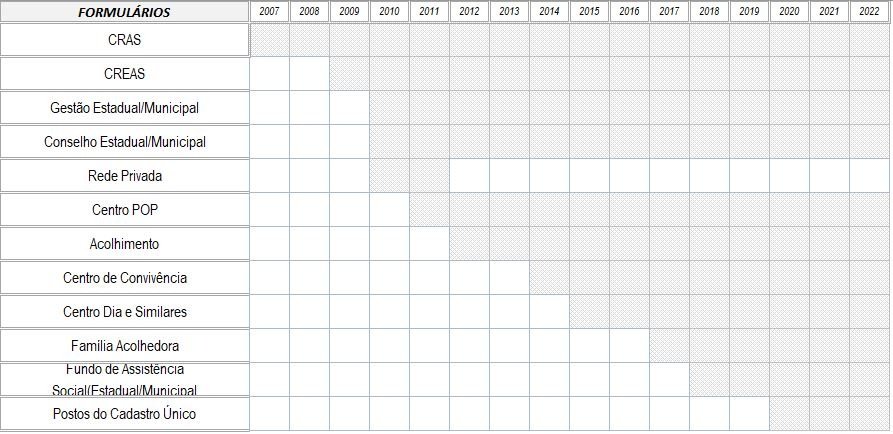
\includegraphics[width=6.5in,height=\textheight]{Imagem_his_censosuas.jpeg}

}

\end{table}%

Ao longo desses dezesseis anos, o Censo tem como principal objetivo
retratar as estruturas de gestão e de oferta de serviços do SUAS,
produzindo informações que subsidiem o planejamento da política, o
aperfeiçoamento do sistema, a formação dos trabalhadores e a prestação
de contas à sociedade. Assim, é possível, a partir de seus resultados,
monitorar e gerar ações e medidas que objetivam a resolução de
dificuldades e o aprimoramento da gestão. Cabe destacar que o Censo SUAS
foi uma das iniciativas premiadas\footnote{Em ENAP (2011)} na publicação
de registro das dez ações premiadas do 16º Concurso Inovação na Gestão
Pública Federal, há um breve relato histórico do Censo SUAS.

Sobre o conteúdo dos formulários destacados na ilustração histórica,
destaca-se os seguintes a partir da última publicação:

\begin{itemize}
\item
  \textbf{Questionário Gestão Municipal:} 8 Blocos, são eles:
  Identificação do Órgão Gestor; Gestão do SUAS; Serviços; Programas e
  outras Ações Socioassistenciais; Benefícios Socioassistenciais,
  CadÚnico e Transferência de Renda; Atuação durante a pandemia de
  Covid-19 e Gestão do Trabalho.
\item
  \textbf{Questionário Gestão Estadual :} 8 Blocos, são eles:
  Identificação do Órgão Gestor; Estrutura Administrativa e Gestão do
  SUAS; Serviços e Benefícios; Regionalização dos Serviços de Média e
  Alta Complexidade; Plano de Providência e Apoio Técnico; Comissão
  Intergestores Bipartite (CIB); Funcionamento durante a pandemia de
  Covid 19 e Gestão do Trabalho.
\item
  \textbf{Questionário Fundo Municipal:} 5 Blocos, são eles:
  Identificação; Gestão de Recursos; Recursos Humanos e Responsável pelo
  preenchimento.
\item
  \textbf{Questionário Fundo Estadual:} 6 Blocos, são eles:
  Identificação; Cofinanciamento Estadual; Índice de Gestão
  Descentralizada do Programa Auxílio Brasil; Gestão de Recursos;
  Recursos Humanos e Responsável pelo preenchimento.
\item
  \textbf{Questionário Centro de Referência de Assistência Social
  (CRAS):} 12 Blocos, são eles: Identificação; Estrutura Física; Serviço
  de Proteção e Atendimento Integral a Família (PAIF); Serviço de
  Convivência e Fortalecimento de Vínculos (SCFV); Serviços de PSB no
  Domicílio para pessoas com Deficiência e idosas; Equipe Volante;
  Benefícios socioassistenciais; Cadastro Único; Programa Auxílio
  Brasil; Funcionamento do CRAS durante a pandemia de Covid 19; Programa
  Criança Feliz; Gestão e Território; Gestão de Pessoas.
\item
  \textbf{Questionário Centro de Convivência:} 5 Blocos, são eles:
  Identificação; Caracterização da Unidade; Serviços e Atividades;
  Gestão; Gestão do trabalho.
\item
  \textbf{Questionário Centro de Referência Especializado de Assistência
  Social (CREAS):} 11 Blocos, são eles: Identificação; Estrutura Física;
  Serviço de Proteção e Atendimento Especializado a Famílias e
  Indivíduos (PAEFI); Serviço de Proteção Social a Adolescentes em
  Cumprimento de Medida Socioeducativa de Liberdade Assistida (LA) e de
  Prestação de Serviços à Comunidade (PSC); Serviço de Abordagem Social;
  Serviço de Proteção Social Especial para Pessoas com Deficiência,
  Idosas e suas Famílias; Benefícios e Cadastro Único; Gestão e
  território; Funcionamento durante a pandemia de Covid-19; Articulação
  e Gestão de Pessoas.
\item
  \textbf{Questionário Centro de Referência Especializado para População
  em Situação de Rua (Centro POP):} 8 Blocos, são eles: Identificação;
  Estrutura Física; Funcionamento durante a pandemia de COVID-19;
  Serviço Especializado para Pessoas em Situação de Rua; Serviço
  Especializado em Abordagem Social; Benefícios, Cadastro Único Gestão e
  Participação de Usuárias/os; Articulação e Gestão de Pessoas.
\item
  \textbf{Questionário do Centro-Dia e similares:} 7 Blocos, são eles:
  Identificação, Caracterização da Unidade, Serviços e atividades;
  Estrutura Física; Perfil dos usuários; Funcionamento durante a
  pandemia de Covid 19; Articulação; Serviços e Atividades e Gestão de
  Pessoas.
\item
  \textbf{Questionário Unidades de Acolhimento:} 7 Blocos, são eles:
  Identificação; Caracterização da Unidade; Características das/os
  usuárias/os; Serviço de Acolhimento; Estrutura Física e Área de
  Localização da Unidade; Funcionamento deste acolhimento durante a
  pandemia de Covid 19 e Recursos Humanos.
\item
  \textbf{Questionário Família Acolhedora:} 4 Blocos, são eles:
  Identificação, Caracteristica das/os Acolhidas/os; Serviços de
  Acolhimento; Funcionamento durante a pandemia de Covid 19; Famílias
  Acolhedoras e Gestão de Pessoas.
\item
  \textbf{Questionário Postos de Cadastro Único:} 4 Blocos, são eles:
  Identificação, Estrutura Física; Cadastro Único; Programa Bolsa
  Família; Outras Atividades; Funcionamento dos postos e Gestão de
  Pessoas.
\item
  \textbf{Questionário Conselhos Municipais de Assistência Social (CMAS)
  e Conselho de Assistência Social do Distrito Federal (CAS/DF):} 10
  Blocos, são eles: Identificação; Regulação; Infraestrutura do
  Conselho; Secretaria Executiva; Orçamento dos Conselhos; Dinâmica de
  Funcionamento; Rede Socioassistencial; Composição do Conselho;
  Conselheiras/os e Responsável pelo Preenchimento.
\item
  \textbf{Questionário Conselhos Estaduais de Assistência Social
  (CEAS):} 10 Blocos, são eles: Identificação; Regulação; Infraestrutura
  do Conselho; Secretaria Executiva; Orçamento dos Conselhos; Dinâmica
  de Funcionamento; Rede Socioassistencial; Composição do Conselho;
  Conselheiras/os e Responsável pelo Preenchimento.
\end{itemize}

Após essa fase de decisão, os formulários são encaminhados para SAGICAD
para processo de tabulação e geração de códigos. É importante destacar
que os códigos das variáveis sofrem mudança conforme alteração das
perguntas (inclusão e exclusão de perguntas). Este torna-se um desafio
para o acompanhamento das respostas ao longo de períodos, haja vista
inexistência de uma chave mestra.

\section{Preenchimento dos
formulários}\label{preenchimento-dos-formuluxe1rios}

A coleta de dados envolve vários agentes públicos municipais e estaduais
das gestões e controle social do SUAS. De acordo com a Norma Operacional
Básica do SUAS / 2012 (NOBSUAS/2012) o processo de realização do Censo
SUAS deve ser coordenado pela vigilância socioassistencial que deve
apoiar no preenchimento zelando pela qualidade das informações
coletadas.

O Censo SUAS 2022 foi realizado, seguindo a tradição anual, por meio de
questionários eletrônicos disponíveis no portal da SAGICAD. O
preenchimento em meio eletrônico é realizado apenas pelos órgãos
gestores (estaduais e municipais) e conselhos de assistência social
(estaduais e municipais). Destaca-se que, para preenchimento dos
questionários, o usuário deve estar devidamente cadastrado na Rede SUAS
e possuir uma senha de acesso. Os questionários, depois de preenchidos,
devem ser salvos pelo respondente. O período de coleta foi entre outubro
e dezembro de 2022, conforme cronograma da Tabela~\ref{tbl-cronograma}.

\begin{longtable}[]{@{}lll@{}}

\caption{\label{tbl-cronograma}Cronograma de preenchimento do Censo SUAS
2022 por questionário.}

\tabularnewline

\toprule\noalign{}
Questionário & Abertura & Encerramento \\
\midrule\noalign{}
\endhead
\bottomrule\noalign{}
\endlastfoot
CRAS & \multirow{11}{=}{06/Out/2022} & \multirow{11}{=}{02/dez/2022} \\
Centros de Convivência \\
CREAS (municipal e estadual) \\
Centro POP \\
Centro-Dia e Similares \\
Unidades de Acolhimento (municipal e estadual) \\
Família Acolhedora \\
Posto de Cadastramento \\
Fundos de Assistência social (municipal e estadual) \\
Gestão (municipal e estadual) \\
Conselhos (municipal e estadual) \\
Período de Retificação & 05/Dez/2022 & 16/Dez/2022 \\

\end{longtable}

\section{Tabulação dos dados e
análise}\label{tabulauxe7uxe3o-dos-dados-e-anuxe1lise}

Aproximadamente 45 mil questionários foram coletadas. Os bancos de dados
resultantes da coleta foram então submetidos a procedimentos de análise
da integridade e consistência, bem como de limpeza de dados e de
organização da estrutura final e da documentação das bases. Para cada
base resultante de um tipo de questionário, foram realizados
procedimentos de limpeza e organização específicos. Inicialmente,
pretendeu-se manter o maior número possível de respondentes válidos.
Para isso, foram considerados como válidos:

\begin{itemize}
\item
  Questionários totalmente preenchidos e devidamente salvos pelos
  respondentes;
\item
  Questionários preenchidos em sua totalidade, mas não devidamente
  salvos por razões de sistema; e
\item
  Questionários preenchidos até 90\% de sua totalidade com pelo menos um
  trabalhador registrado no bloco de Recursos Humanos do questionário.
\end{itemize}

A análise dos resultados do Censo SUAS 2022 compreende o SUAS como
política social por meio dos componentes sistêmicos da PNAS, conforme
seu estágio de institucionalização. Para essa versão consideramos
destaques do II Plano Descenal. A tentativa é aprofundar da compreensão
universal do SUAS. A exposição da análise do Censo SUAS será realizada
de acordo com seis eixos de análise, a saber\footnote{A forma de
  organização processual destas informações foram através do ``R
  Markdown''. Tal metodologia foi inovadora para o ano de 2022 que antes
  era realizado a partir de planilhas e gráficos gerados pelo excel. Tal
  percurso representa maior confiabilidade nas informações, amplia as
  possibilidades de produção de gráficos, ganho no tempo para próximas
  publicações entre outras.}:

\begin{itemize}
\item
  \textbf{Gestão e Financiamento do Sistema Único de Assistência
  Social:} panorama geral da gestão e do financiamento em estados e
  municípios, com a observação de aspectos como a estrutura
  administrativa da gestão da assistência social, a atualização de
  normativos, o apoio de estados aos municípios, as atividades de
  cofinanciamento e transferência de recursos, funcionamento das
  instâncias de pactuação, entre outras.
\item
  \textbf{Unidades, Serviços e Benefícios da Assistência Social:}
  apresenta informações a respeito dos equipamentos da Assistência
  Social e sua evolução ao longo do tempo, sua estutura e condições na
  perspectiva de acessibilidade e equipamentos disponíveis. A integração
  dos Serviços do SUAS no âmbito das proteções sociais, relação com o
  Cadastro Único, Benefícios do SUAS, bem como Programas. Também
  aborda-se sobre a Regionalização da proteção social Especial.
\item
  \textbf{Recursos Humanos do SUAS:} apresenta um panorama geral da
  situação das trabalhadoras e trabalhadores do SUAS tanto nos
  equipamentos da assistência social quanto nas gestões municipais e
  estaduais, apresentando informações sobre quantitativo, tipo de
  vínculo trabalhista, escolaridade, entre outros aspectos referentes à
  gestão do trabalho, e sua evolução ao longo dos anos.
\item
  \textbf{Participação e controle social no SUAS:} apresenta os
  resultados apurados pelo Censo SUAS para os Conselhos Municipais e
  Estaduais de Assistência Social, considerando a estrutura
  administrativa, a dinâmica de funcionamento e a composição.
\end{itemize}

Espera-se que, a partir de uma avaliação com abordagem direcionada à
análise integrada do SUAS e partindo dos dados dos órgãos de gestão das
unidades de atendimento públicas e privadas e das instâncias
administrativas e deliberativas, seja possível retratar o seu
funcionamento e evolução como política social. Assim, amplia-se a
compreensão acerca da rede de assistência social por parte dos gestores,
trabalhadores e sociedade civil, permitindo uma apreensão crítica de seu
funcionamento.

\bookmarksetup{startatroot}

\chapter{Gestão e Financiamento}\label{gestuxe3o-e-financiamento}

O Sistema Único de Assistência Social (SUAS) é definido pela Lei
Orgânica da Assistência Social (LOAS)\footnote{Lei nº 8.742, de 7 de
  dezembro de 1993: Dispõe sobre a organização da Assistência Social e
  dá outras providências.
  (\url{http://www.planalto.gov.br/ccivil_03/Leis/L8742compilado.htm})}
como um sistema descentralizado e participativo que organiza a gestão
das ações na área de assistência social, a partir das diretrizes:
descentralização político administrativa, participação social e primazia
da responsabilidade do Estado na condução da política de assistência
social. Assim, tem como um de seus objetivos a consolidação da gestão
compartilhada dos três entes federados.

A LOAS, a NOB SUAS\footnote{Norma Operacional Básica NOB - SUAS 2012
  (\url{http://www.mds.gov.br/webarquivos/arquivo/assistencia_social/nob_suas.pdf})}
e outros normativos que regulam a assistência social definem as
responsabilidades da União, Estados, Distrito Federal e Municípios no
âmbito da gestão compartilhada, que incluem o cofinanciamento de
serviços, programas e ações da assistência social. Estão previstas ainda
instâncias de pactuação e interlocução entre os três entes federados: a
Comissão Intergestores Bipartite (CIB), da qual participam
representantes de estados e municípios, e a Comissão Intergestores
Tripartite (CIT), da qual participam, além de estados e municípios,
representantes do governo federal.

\section{Estrutura Administrativa normas e
planejamento}\label{estrutura-administrativa-normas-e-planejamento}

A partir das informações contidas no Censo SUAS é possível ter um
panorama geral da gestão e do financiamento em estados e municípios, com
a observação de aspectos como a estrutura administrativa da gestão da
assistência social, a atualização de normativos, o apoio de estados aos
municípios, as atividades de cofinanciamento e transferência de
recursos, funcionamento das instâncias de pactuação, entre outras. Nesse
sentido, esta seção apresenta os principais resultados obtidos a partir
das informações dos questionários de gestão estadual e gestão municipal.

A estrutura administrativa na Política de Assistência Social e
Constituição de setores essenciais são elementos importantes para gestão
do SUAS. No âmbito da gestão estadual, no que se refere a exclusividade
da área de Assistência Social, percebe-se que nos últimos 10 anos houve
uma redução de áreas específicas de Assistência Social. Em 2012 existiam
29,6\%\footnote{Estados: Amazonas, Acre, Pará, Amapá, Piauí, Paraíba,
  Sergipe e São Paulo} das secretarias estaduais exclusivas de
Assistência Social, em 2022 esse número passa para 3,8\%\footnote{Estado
  do Amazonas}, redução significativa de 87,2\%, conforme o
Gráfico~\ref{fig-estados_sec_exc}.

\begin{figure}

\centering{

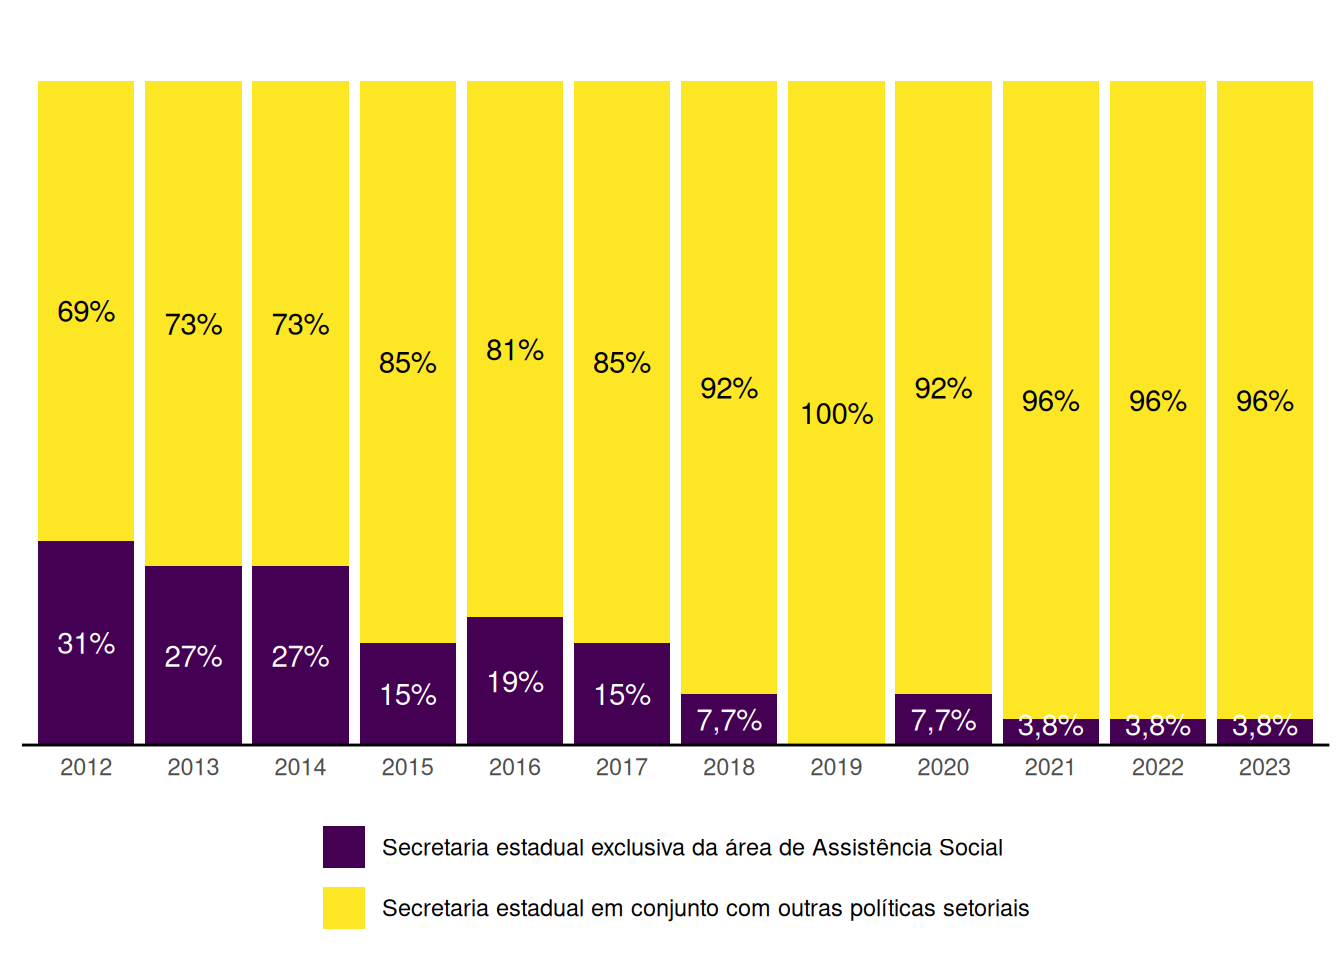
\includegraphics{gestao_files/figure-pdf/fig-estados_sec_exc-1.pdf}

}

\caption{\label{fig-estados_sec_exc}Percentual de Estados quanto a
caracteristica de estrutura administrativa - Brasil, 2012 a 2022}

\end{figure}%

No que se refere aos municípios, esse cenário nacional se configurou
inverso ao das gestões Estaduais. Observa-se através do
Gráfico~\ref{fig-sec-munic-exc} um aumento de 217 municípios (1,5 pontos
percentuais) com secretarias exclusivas de Assistência Social do período
de 2012 a 2019\footnote{a partir de 2019 essa pergunta foi retirada do
  formulário de gestão municipal}.

\begin{figure}

\centering{

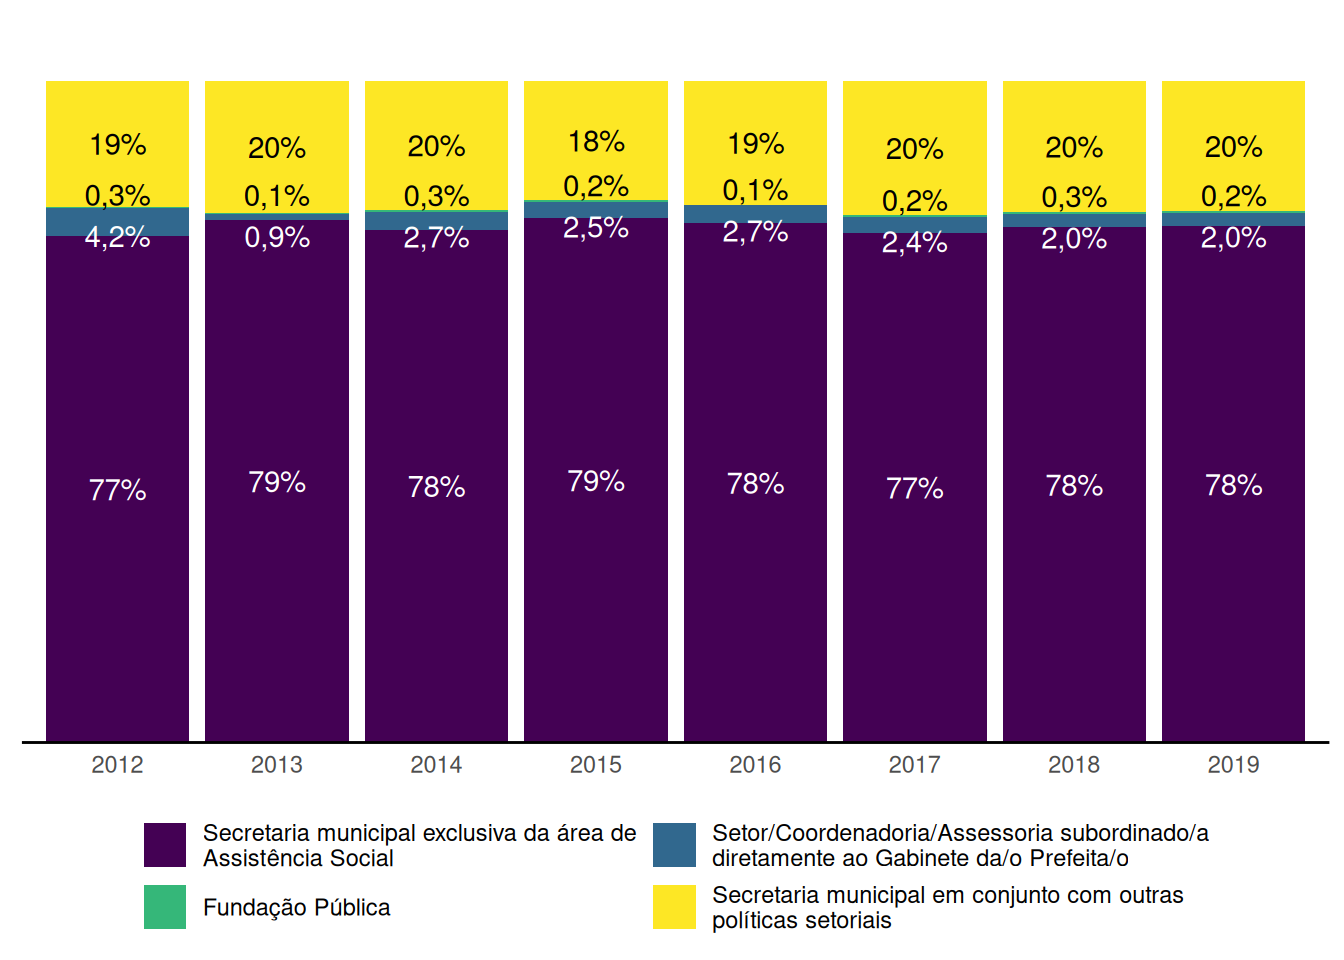
\includegraphics{gestao_files/figure-pdf/fig-sec-munic-exc-1.pdf}

}

\caption{\label{fig-sec-munic-exc}Percentual de Secretarias Municipais
quanto a caracteristica de estrutura administrativa - Brasil, 2012 a
2019}

\end{figure}%

Alguns órgãos gestores estaduais constituíram as áreas de assistência
social como subdivisões administrativas em sua estrutura, como
superintendências, departamentos, gerências, coordenações, dentre
outras. De acordo com o último Pacto de aprimoramento Estadual do
SUAS\footnote{Resolução CNAS Nº2, de 16 de março de 2017} umas das
prioridades para o aperfeiçoamento institucional é possuir na estrutura
administrativa das seguintes áreas:

\begin{enumerate}
\def\labelenumi{\arabic{enumi})}
\tightlist
\item
  Proteção Social Básica;
\item
  Proteção Social Especial de Média e Alta Complexidade;
\item
  Gestão do SUAS, com suas subdivisões de Vigilância Socioassistencial,
  Regulação do SUAS e Gestão do Trabalho; e
\item
  Gestão do Fundo Estadual de Assistência Social - FEAS.
\end{enumerate}

Observa-se avanço em todas as areas formalmente nos últimos 10 anos. As
três áreas mais instituídas formalmente são: Proteção Social Básica e
Proteção Social Especial, com 88\%, e Gestão do SUAS, com 85\%
(Gráfico~\ref{fig-uf_subd}).

\begin{figure}

\centering{

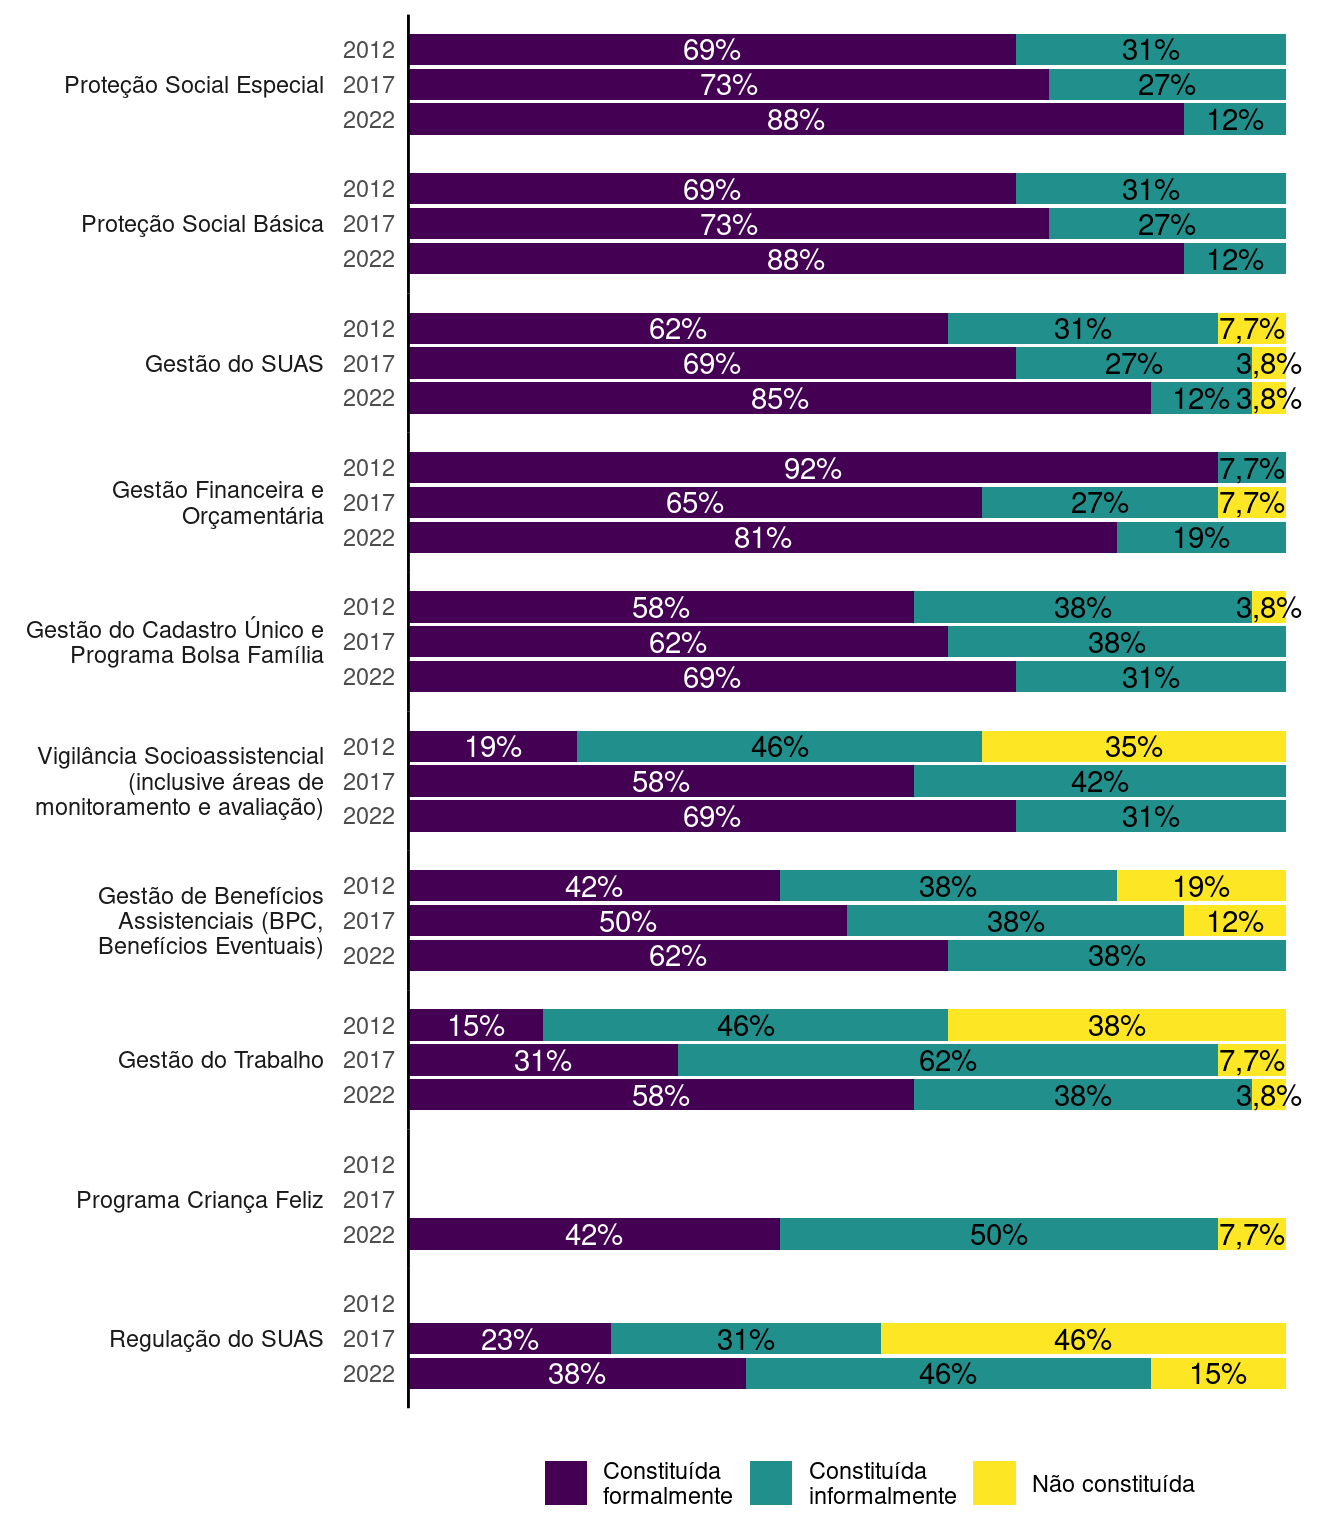
\includegraphics{gestao_files/figure-pdf/fig-uf_subd-1.pdf}

}

\caption{\label{fig-uf_subd}Percentual de estados segundo constituição
de subdivisões administrativas na estrutura do órgão gestor - Brasil;
2012, 2017 e 2022}

\end{figure}%

Quando se observa a regularização destas áreas, há um grupo instituídas
informalmente conforme o
Gráfico~\ref{fig-estados-constituicao-subdivisoes}, e setores que ainda
não estão consituídos em 100\% dos estados, a saber Gestão do SUAS,
Gestão do trabalho e regulação do SUAS.

\begin{figure}

\centering{

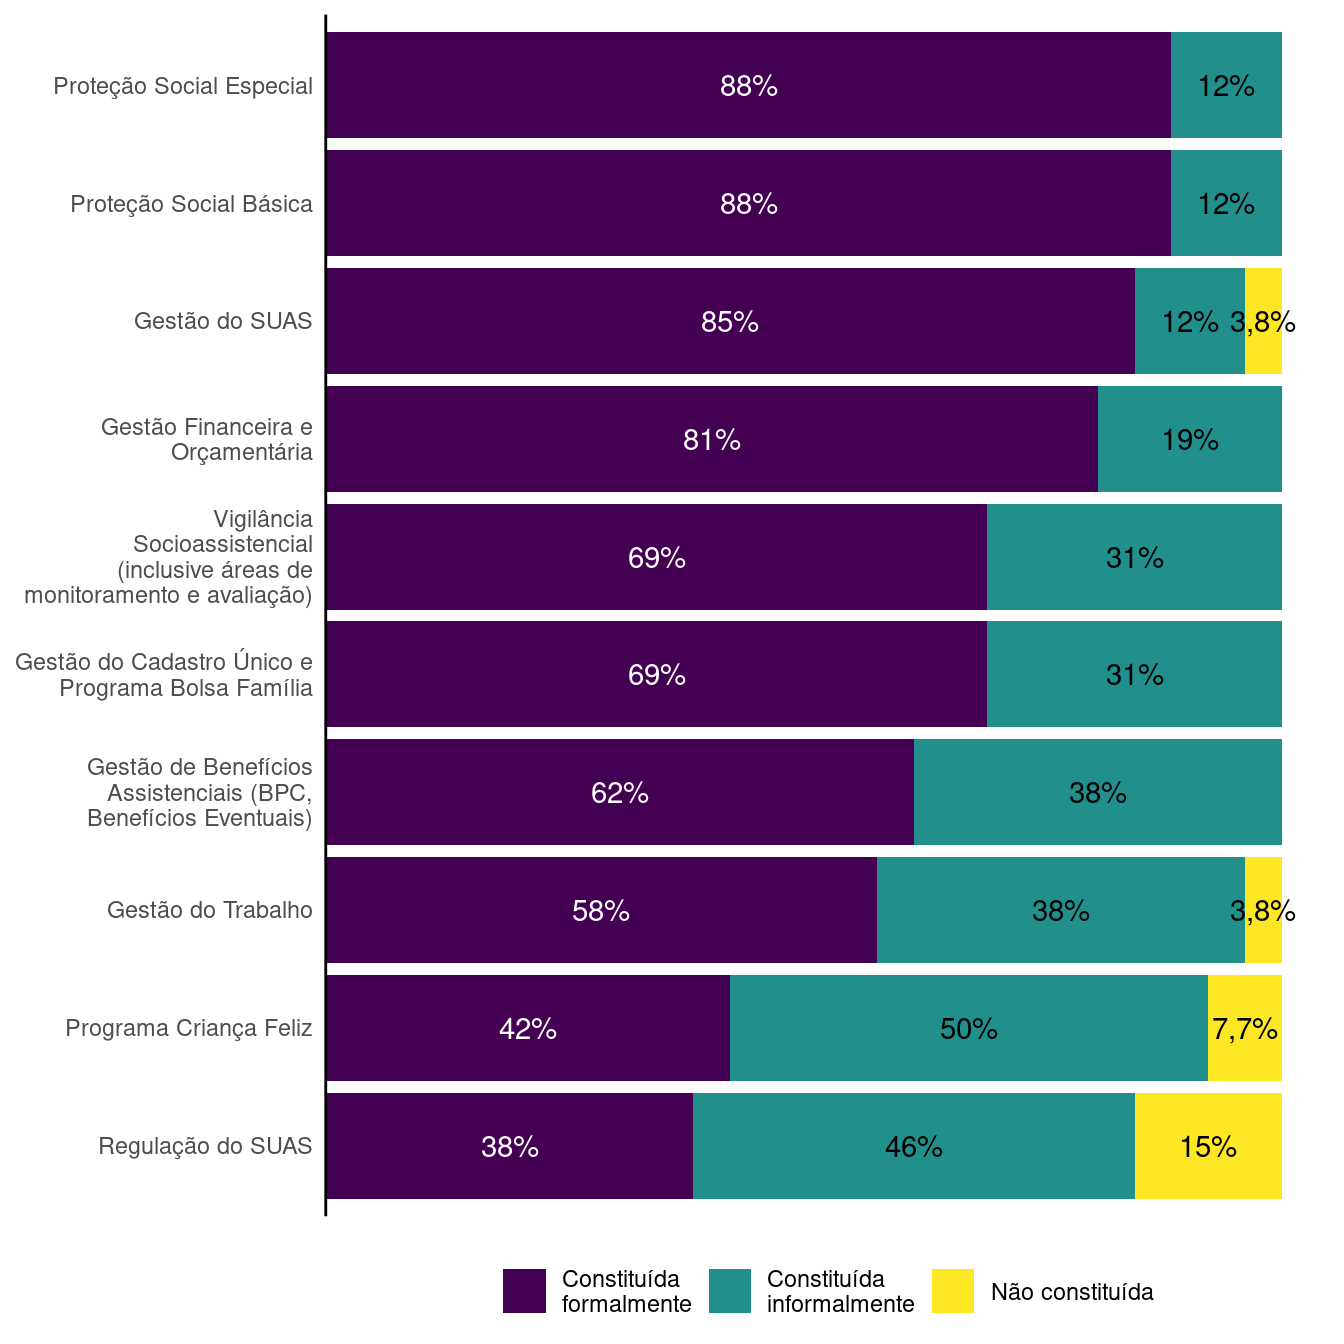
\includegraphics{gestao_files/figure-pdf/fig-estados-constituicao-subdivisoes-1.pdf}

}

\caption{\label{fig-estados-constituicao-subdivisoes}Percentual de
estados segundo característica da estrutura administrativa da Secretaria
Estadual de Assistência Social - Brasil, 2022}

\end{figure}%

No que se refere aos municípios, a última pactuação sobre estrutura
administrativa a partir dos portes populacionais dos
municípios\footnote{124ª reunião ordinária da CIT - Pacto de
  Aprimoramento do SUAS} prevê:

\begin{itemize}
\item
  \textbf{municípios de pequeno I e II e médio porte:} 100\% dos
  municípios com instituição formal, na estrutura do órgão gestor de
  assistência social, as áreas constituídas de Proteção Social Básica,
  Proteção Social Especial e a área de Gestão do SUAS com competência de
  Vigilância Socioassistencial.
\item
  \textbf{municípios de grande porte e metrópole:} 100\% dos muncípios
  com instituição formal, na estrutura do órgão gestor de assistência
  social, áreas constituídas de Proteção Social Básica, Proteção Social
  Especial, com subdivisão de Média e Alta Complexidade, Gestão
  Financeira e Orçamentária, Gestão de Benefícios Assistenciais e
  Transferência de Renda, área de Gestão do SUAS com competência de:
  Gestão do Trabalho, Regulação do SUAS e Vigilância Socioassistencial.
\end{itemize}

O Gráfico~\ref{fig-munic_sub} mostra crescimento formal de todas as
areas administrativas. As areas do SUAS com maior percentual de
constituição formal\footnote{A regulamentação destas areas essenciais
  devem estar previstas no organograma. A Lei do SUAS Lei nº 12.435, de
  06/07/2011 altera a Lei Organiza da Assistência Social (LOAS) - nº
  8.742, de 07/.12.1993} que dispõe sobre esta organização são
respectivamente: Gestão do Cadastro Único e Bolsa Família, Gestão da
Proteção Social Básica e Gestão do SUAS.

\begin{figure}

\centering{

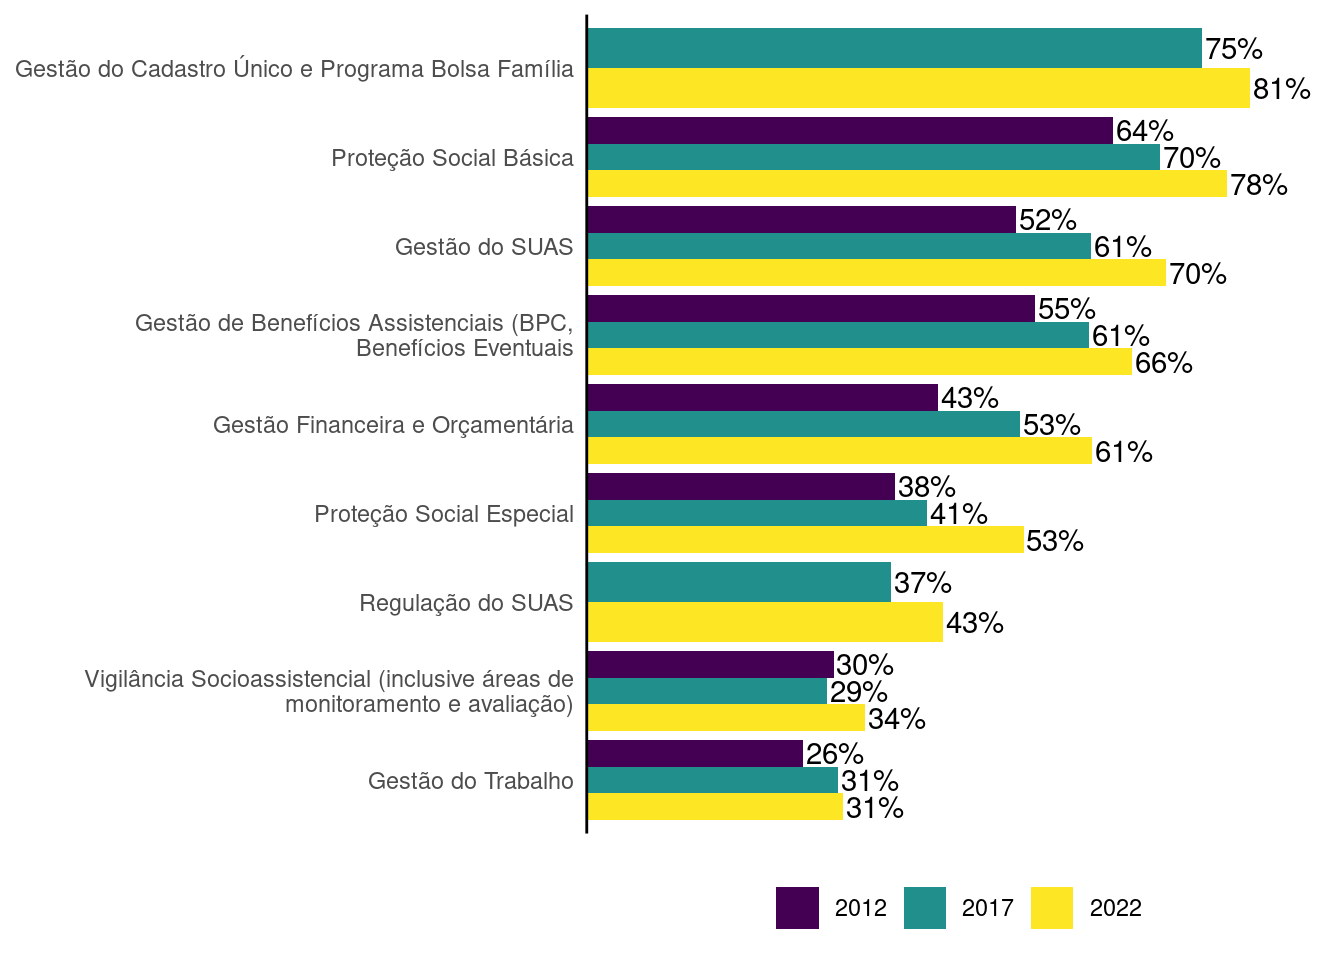
\includegraphics{gestao_files/figure-pdf/fig-munic_sub-1.pdf}

}

\caption{\label{fig-munic_sub}Percentual segundo estrutura
administrativa formal da Secretaria Municipal de Assistência Social -
Brasil, 2012 - 2017 - 2022}

\end{figure}%

Ao considerar a instituição informal, o
Gráfico~\ref{fig-municipais-constituicao-subdivisoes} sinaliza que a
Gestão do trabalho e Vigilância Socioassistencial são os mais altos
percentuais de informalidade e não constituição. Destaca-se também a
proteção social especial, área recomendada existir independe da presença
de unidades de CREAS.

\begin{figure}

\centering{

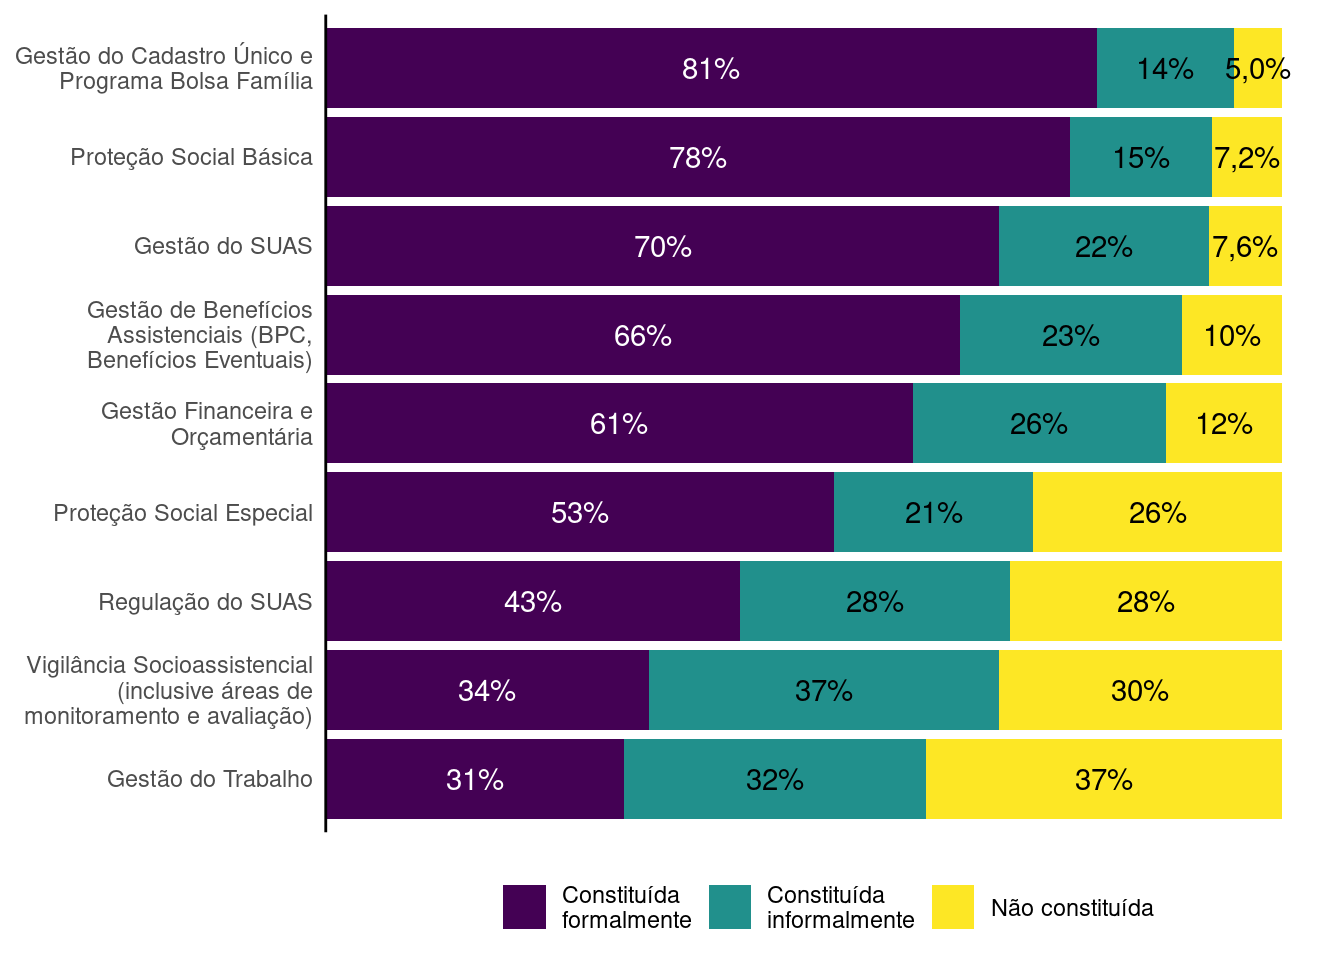
\includegraphics{gestao_files/figure-pdf/fig-municipais-constituicao-subdivisoes-1.pdf}

}

\caption{\label{fig-municipais-constituicao-subdivisoes}Distribuição dos
órgãos gestores municipais segundo constituição/formalização de
subdivisões administrativas - Brasil, 2022}

\end{figure}%

A uniformização da Lei do SUAS dos estados e municípios em consonâcia
com a LOAS foi deliberação da X Conferência Nacional. Sobre essa
disposição, observa-se que nas gestões estaduais, 58\% dos estados
possuem Lei Estadual de regulamentação do SUAS (total de 15 estados). As
últimas atualizações ocorreram a partir de 2017 (12 estados), com
exceção de Minas Gerais em 2011 Goiás em 2015 e Mato Grosso do Sul em
2016.

Entretando, 11 estados que não possuem Lei do SUAS. Este número está
presente nas seguintes regiões do Brasil: 4 - Nordeste, 3 - Norte, 2 -
Região Sul e 1 - Região Sudeste. Sudeste\footnote{siglas dos Estado que
  não possuem Lei do SUAS - Censo SUAS 2022: RR, PA, TO, PI, RN, SE, BA,
  SP, PR, SC e RS}.

\begin{figure}

\centering{

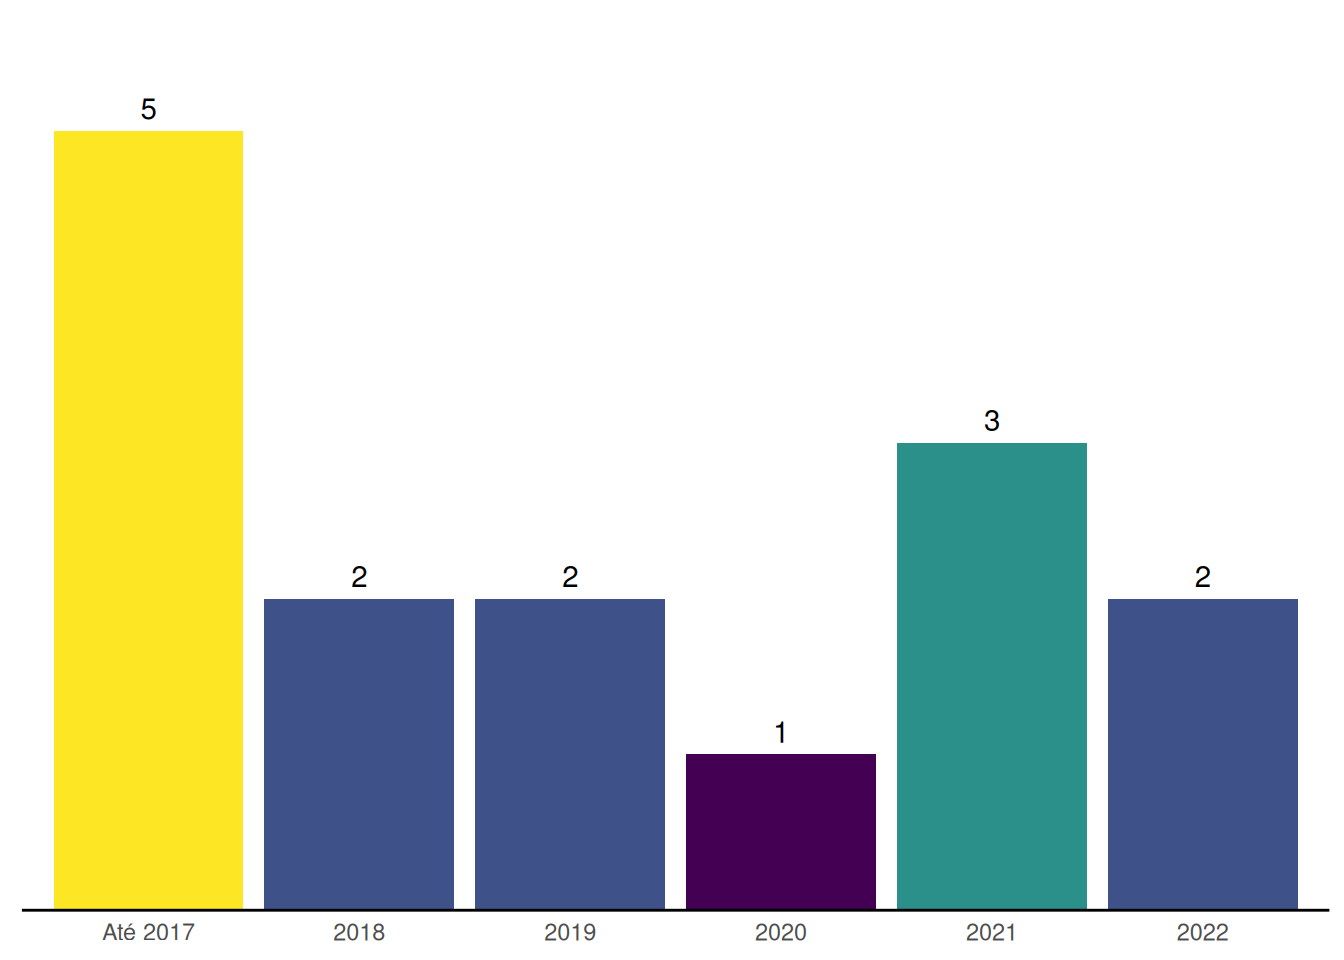
\includegraphics{gestao_files/figure-pdf/fig-estados-atualizacao-lei-1.pdf}

}

\caption{\label{fig-estados-atualizacao-lei}Quantidade de estados
segundo último ano de atualização da Lei Estadual de regulamentação do
Sistema Único de Assistência Social (SUAS) - Brasil, 2022}

\end{figure}%

Em 2022, 75\% dos municípios possuíam Lei Municipal de regulamentação do
SUAS (4.170). Destes, a maioria, 91\% (3.798) aprovaram/atualizaram após
2013 e 9\% (372) anterior a atualização da Lei Nacional\footnote{Lei nº
  12.435, de 06/07/2011 altera a Lei Organiza da Assistência Social
  (LOAS) - nº 8.742, de 07/.12.1993} e a NOB SUAS/2012 conforme detalha
o Gráfico~\ref{fig-municipios-atualizacao-lei}. A inexistência de Lei é
encontrada em 25\% (1.400) dos municípios.

\begin{figure}

\centering{

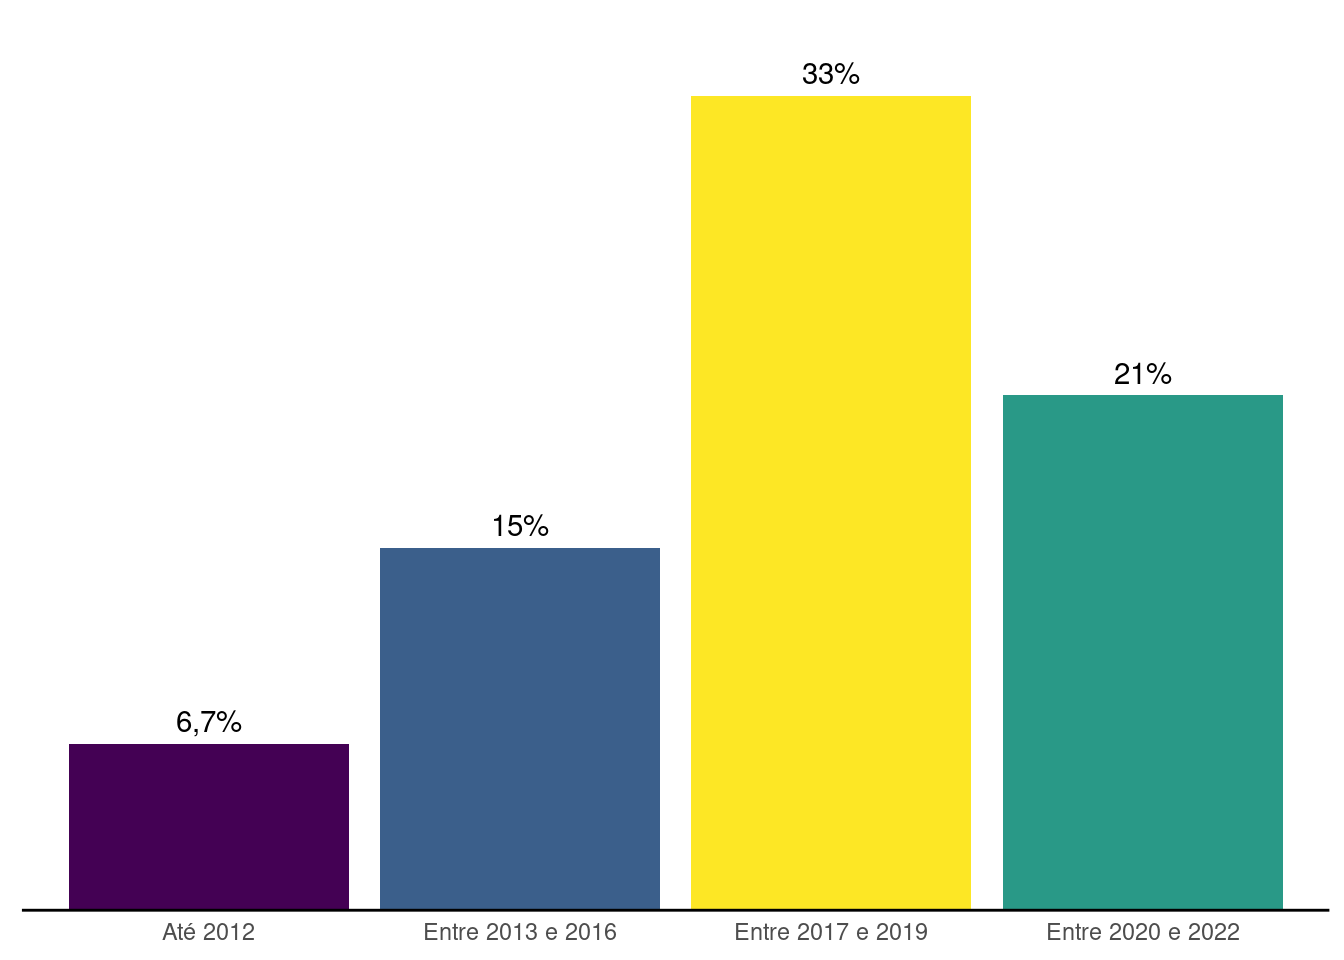
\includegraphics{gestao_files/figure-pdf/fig-municipios-atualizacao-lei-1.pdf}

}

\caption{\label{fig-municipios-atualizacao-lei}Percentual de municípios
segundo último ano de atualização da Lei Municipal de regulamentação do
Sistema Único de Assistência Social (SUAS) - Brasil, 2022}

\end{figure}%

No que se refere ao Planejamento, trata-se de uma obrigatoriedade para
existência do Sistema Único e repasse de confinanciamento. O Plano
Estadual de Assistência Social (PEAS) deve ser aprovado pelo Conselho
Estadual de Assistência Social (CEAS). Os dados do
Gráfico~\ref{fig-PEAS} sinalizam que a partir de 2020 há um decréscimo
desta atualização com devida aprovação do conselho\footnote{Para os anos
  de 2016, 2017, 2018 e 2019 as perguntas alteraram, impossibilitando a
  linha histórica} \footnote{Para os municípios não foi possível fazer
  essa linha histórica em decorrência de mudanças nas perguntas}.

\begin{figure}

\centering{

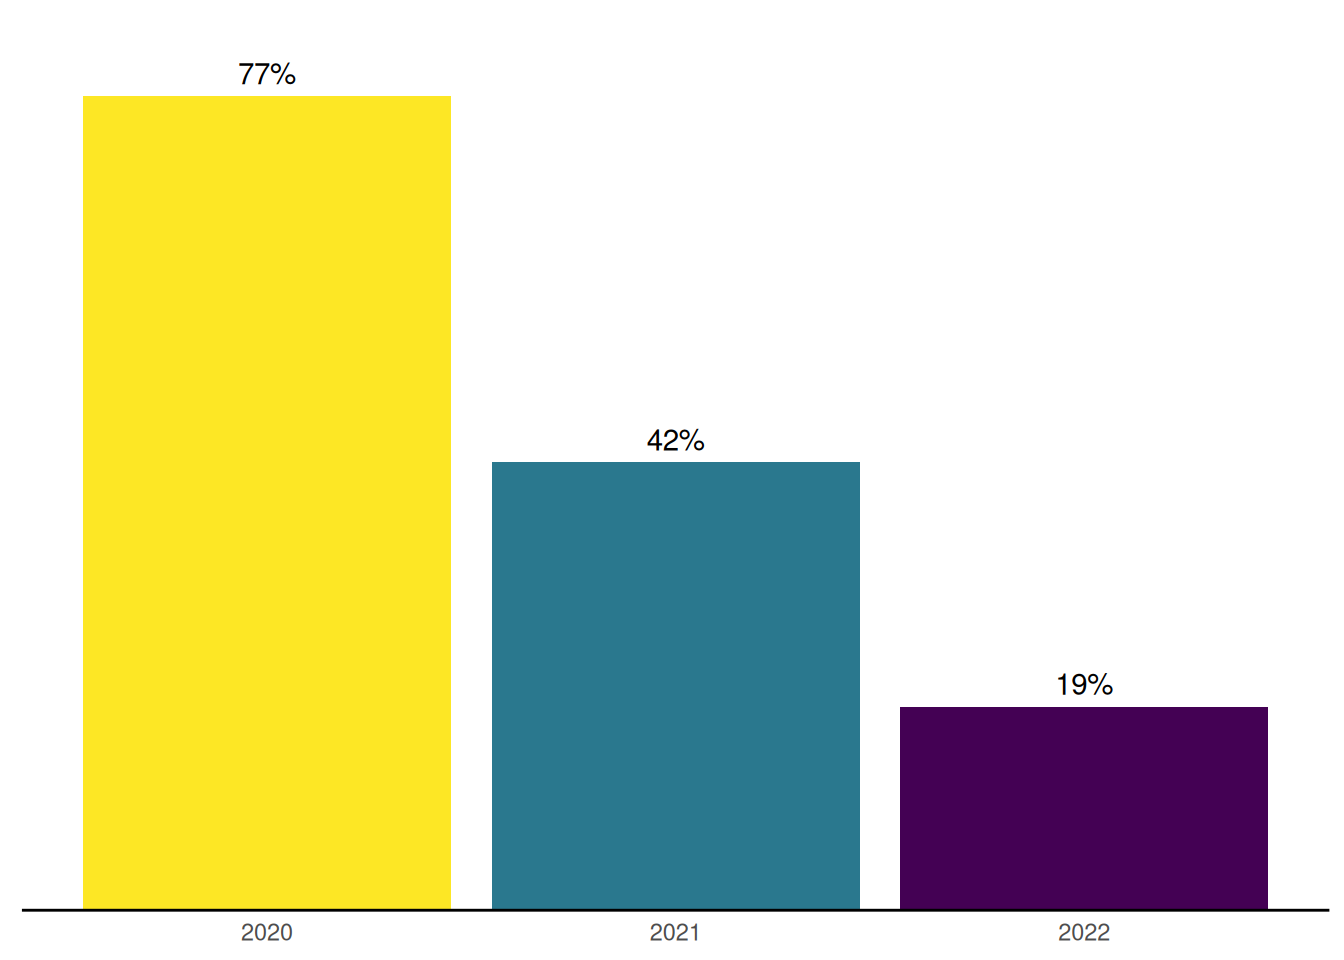
\includegraphics{gestao_files/figure-pdf/fig-PEAS-1.pdf}

}

\caption{\label{fig-PEAS}Percentual de Estados quanto a atualização do
Plano Estadual de Assistência Social no ano do Censo - Brasil, 2020 a
2022}

\end{figure}%

O Plano de apoio técnico aos municípios também é um produto a ser
realizado pelos Estados e previsto no último pacto de aprimoramento
Estadual do SUAS\footnote{Resolução CNAS Nº2, de 16 de março de 2017}.
De acordo com Censo Suas 2022, 57,69\% dos Estados possuem este plano
pactuado na CIB. Este percentual reduziu em relação ao ano de 2017, na
qual mais de 77\% dos estados informaram possuir este documento pactuado
nesta instância de comissão intergestores bipartite (CIB).

\begin{figure}

\centering{

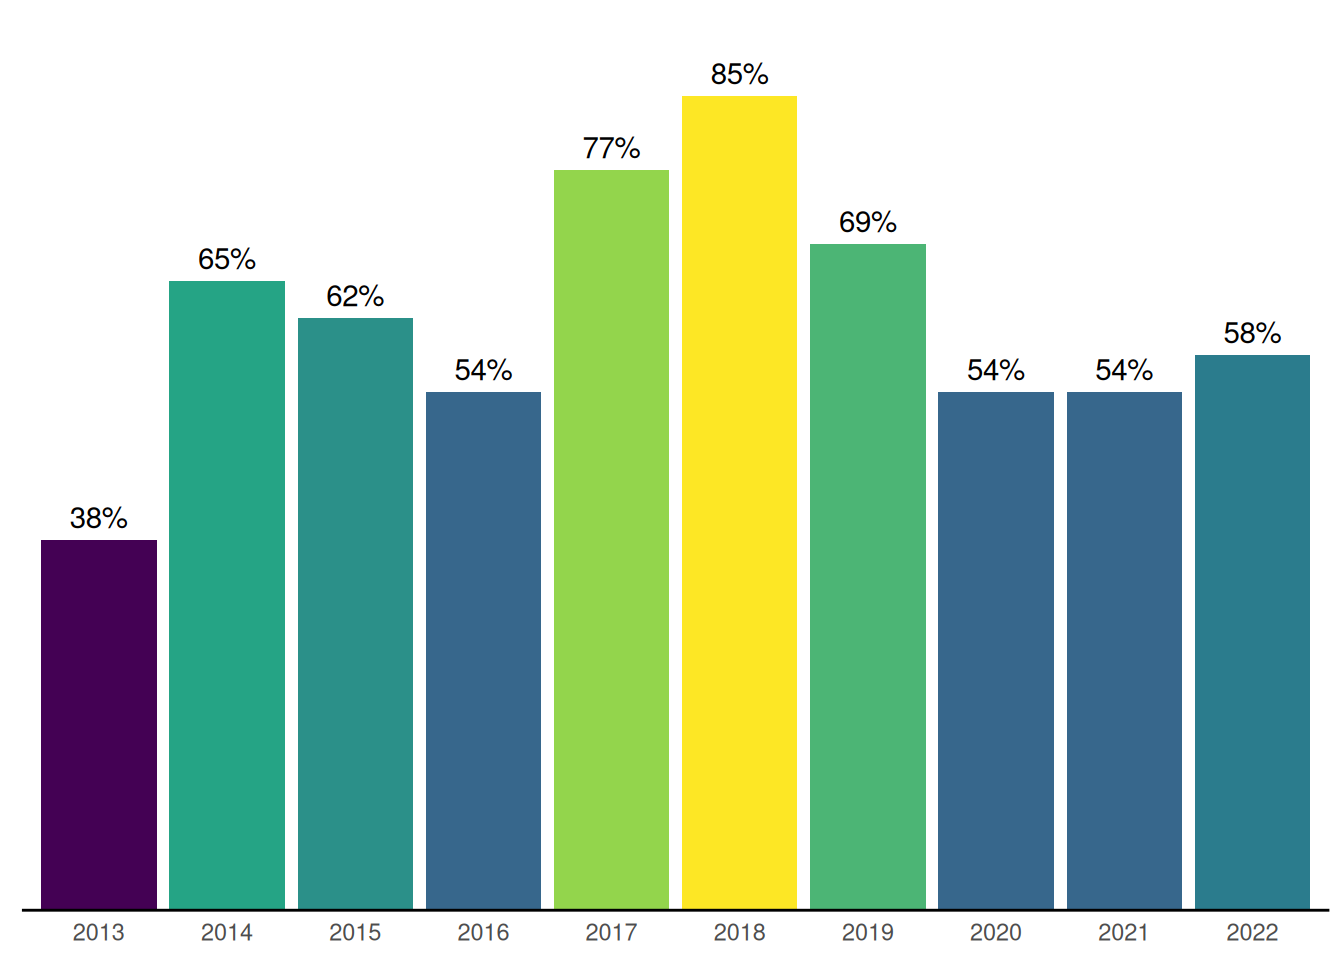
\includegraphics{gestao_files/figure-pdf/fig-plan_apoio_tec-1.pdf}

}

\caption{\label{fig-plan_apoio_tec}Percentual de Estados que possuem
Plano de Apoio Técnico pactuado na CIB - Brasil, 2013 a 2022}

\end{figure}%

A NOB SUAS 2012 também evidencia o papel dos estados frente as
atribuições de apoio técnico e financeiro aos municípios\footnote{Capítulo
  III - NOBSUAS/2012} na qual compreende ações de:

\begin{enumerate}
\def\labelenumi{\Roman{enumi})}
\tightlist
\item
  Capacitação;
\item
  Elaboração de normas e instrumentos;
\item
  Publicação de materiais informativos e de orientações técnicas;
\item
  Assessoramento e acompanhamento; e
\item
  Incentivos financeiros.
\end{enumerate}

Em 2022, todos os estados informaram realizar alguma modalidade de apoio
técnico aos municípios. Os maiores percentuais observados referiam-se ao
Apoio Técnico individualizado a municípios específicos ofertado por
96,2\% dos estados (25). Os menores percentuais eram referentes a
Seminários 46,2\%, (12). Outras formas eram ofertadas por 15,4\% dos
estados (Gráfico~\ref{fig-estados-formas-apoio}).

Entre 2013 e 2022 o percentual de estados que prestavam assessoramento
técnico a distância aumentou significativamente, passando de 42,3\     (11)
em 2013 para 92,3\% (24) em 2022.

\begin{figure}

\centering{

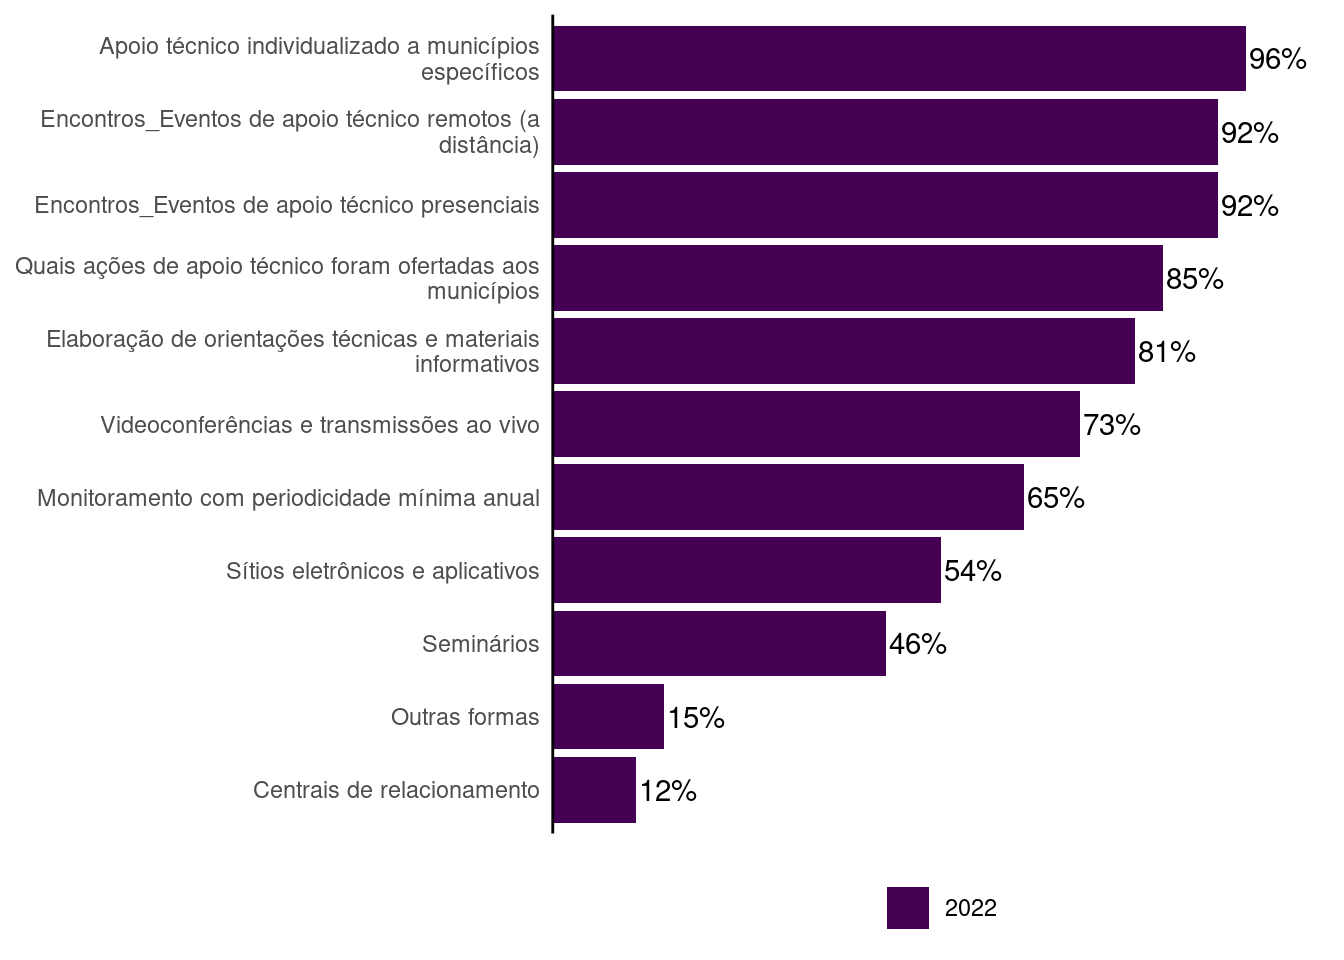
\includegraphics{gestao_files/figure-pdf/fig-estados-formas-apoio-1.pdf}

}

\caption{\label{fig-estados-formas-apoio}Percentual de estados segundo
formas de apoio técnico aos municípios - Brasil, 2022}

\end{figure}%

No Gráfico~\ref{fig-munic_vit_estadual} os dados percentuais mostram um
aumento gradual dos municípios que informam receber visitas da gestão
estadual para apoio técnico. Entretanto 62,5\% informam não ter recebido
visita de apoio técnico no último ano.

\begin{figure}

\centering{

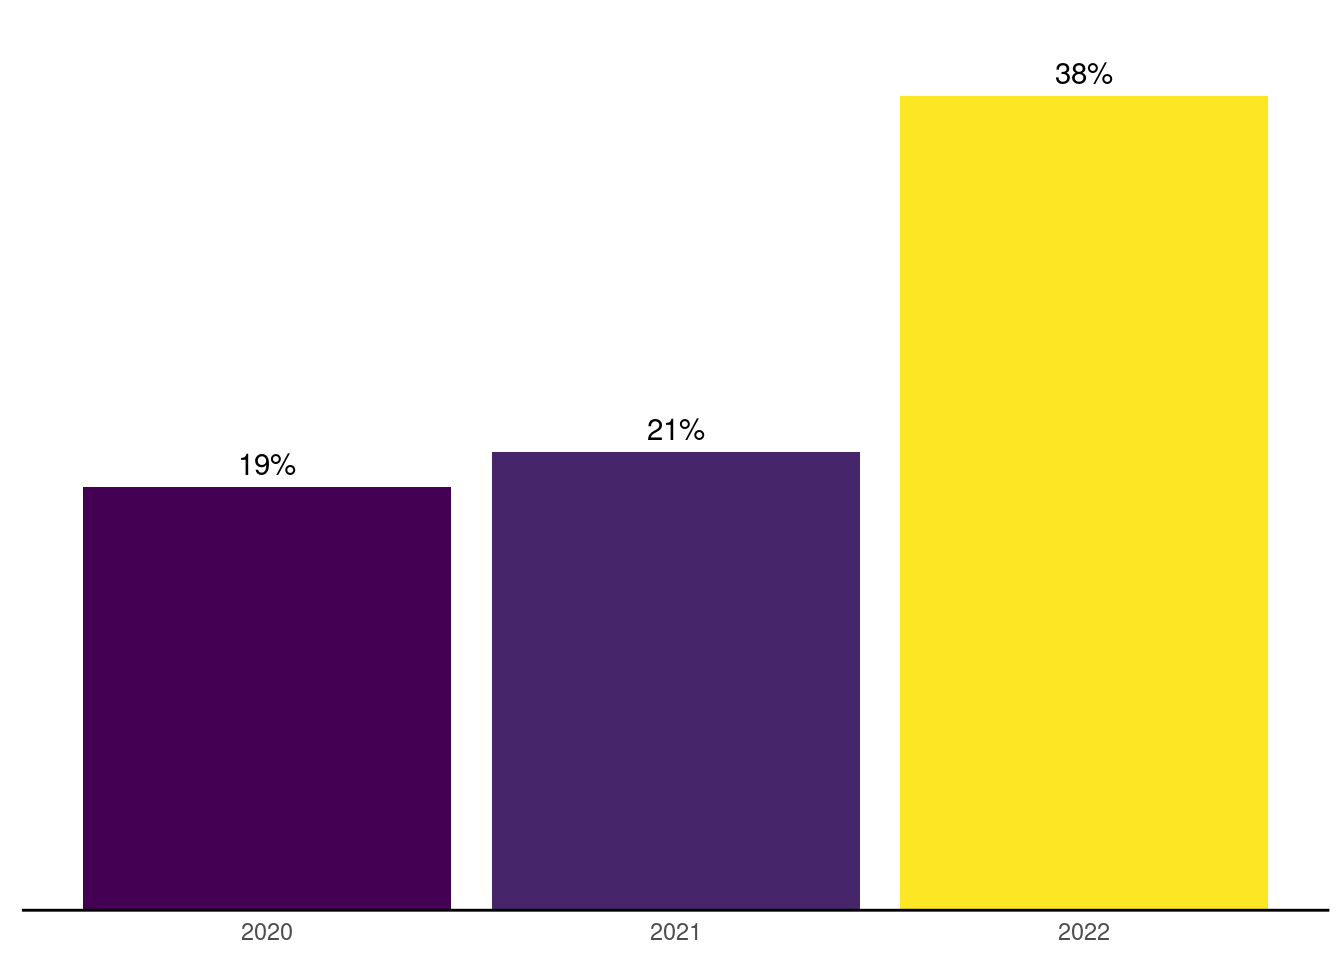
\includegraphics{gestao_files/figure-pdf/fig-munic_vit_estadual-1.pdf}

}

\caption{\label{fig-munic_vit_estadual}Percentual de Municípios que
informam receber visitas de Apoio Técnico do Estado - Brasil, 2020 a
2022}

\end{figure}%

No que se refere a Educação Permanente, nota-se um aumento dos estados
que possuem Núcleo de Educação Permante (Gráfico~\ref{fig-NUEP}).

O censo de 2022 sinaliza 88,5\% (23) dos Estados possuem esta instância
colegiada de maneira formal. Trata-se de um foro constituído pela
participação e cooperação institucionalizada de gestores, trabalhadores,
usuários, conselheiros de assistência social, e instituições de ensino,
pesquisa e extensão. O objetivo é deliberar sobre a implementação
continuada da Política de educação permanente do SUAS.

\begin{figure}

\centering{

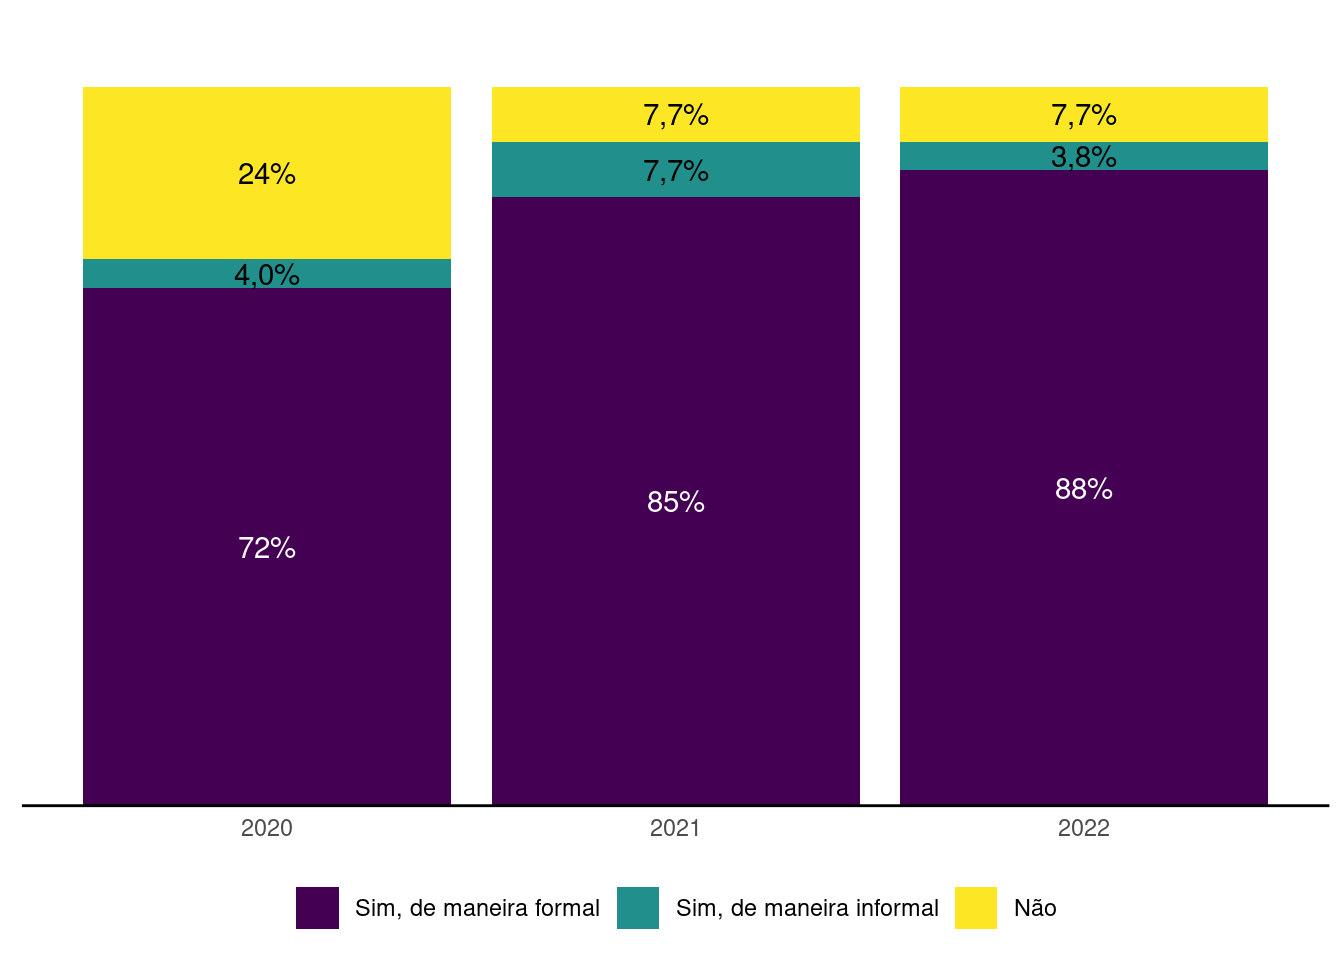
\includegraphics{gestao_files/figure-pdf/fig-NUEP-1.pdf}

}

\caption{\label{fig-NUEP}Percentual de Estados que possuem Núcleo de
Educação Permanente, 2020 a 2022}

\end{figure}%

Em relação ao Plano de Educação Permanente, de acordo com Censo SUAS de
2021, 13,9\% (769) dos municípios possuem este plano. Esse percentual,
como pode ser observado no Gráfico~\ref{fig-PNEP_Munic}, teve evolução
residual últimos anos\footnote{Para o ano de 2022 essa pergunta foi
  extinta}.

\begin{figure}

\centering{

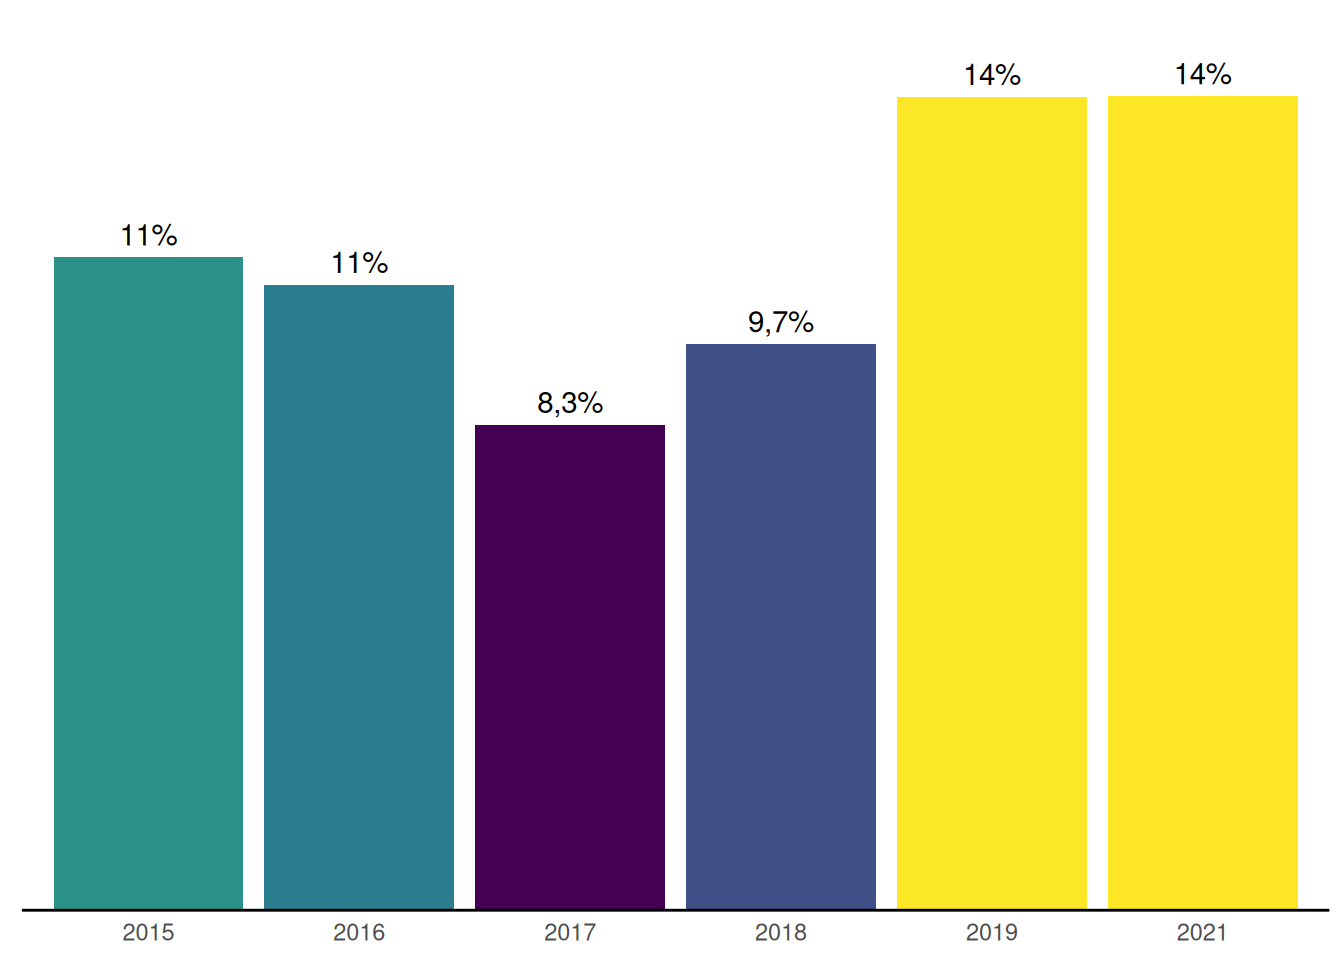
\includegraphics{gestao_files/figure-pdf/fig-PNEP_Munic-1.pdf}

}

\caption{\label{fig-PNEP_Munic}Percentual de municípios que possuem
Plano de Capacitação e Educação Permanente, - Brasil; 2015 a 2019 e
2021}

\end{figure}%

\section{Financiamento e Gestão
Financeira}\label{financiamento-e-gestuxe3o-financeira}

O modelo de gestão do SUAS preve cofinanciamento compartilhado entre os
três entes federados\footnote{Art. 30-A. O cofinanciamento dos serviços,
  programas, projetos e benefícios eventuais, no que couber, e o
  aprimoramento da gestão da política de assistência social no Suas se
  efetuam por meio de transferências automáticas entre os fundos de
  assistência social e mediante alocação de recursos próprios nesses
  fundos nas 3 (três) esferas de governo.}.

Nesta perspetiva, percebe-se um avanço nos últimos 10 anos sobre a
participação dos estados no cofinanciamento estadual com participação de
96,15\% (25) dos estados que informam cofinanciar os municípios
(Gráfico~\ref{fig-estados-cofinanciamento-municipios}).

A forma de cofinanciamento deve ser viabilizada por meio de
transferência automática regular entre os fundos de assistência social
(Fundo a Fundo). Sobre esse item, observa-se que em 2012, 26,63\        (8)
dos estados realizavam cofinanciamento na modalidade de apenas Fundo a
Fundo e 25,9\% (7) apenas por convenio. Dado que avançou ao longo dos
anos, em 2022, 88,46\% (23) dos estados que realizam cofinanciamneto
regular e automático e nenhum estado apenas por convênio.

Apesar destes avanços, há registros de não cofinanciamento estadual, no
qual caiu de 25,93\% (7) no ano de 2012 para 3,85\% (1) em 2022
(1)\footnote{o Estado do Acre não cofinancia os municípios}.

\begin{figure}

\centering{

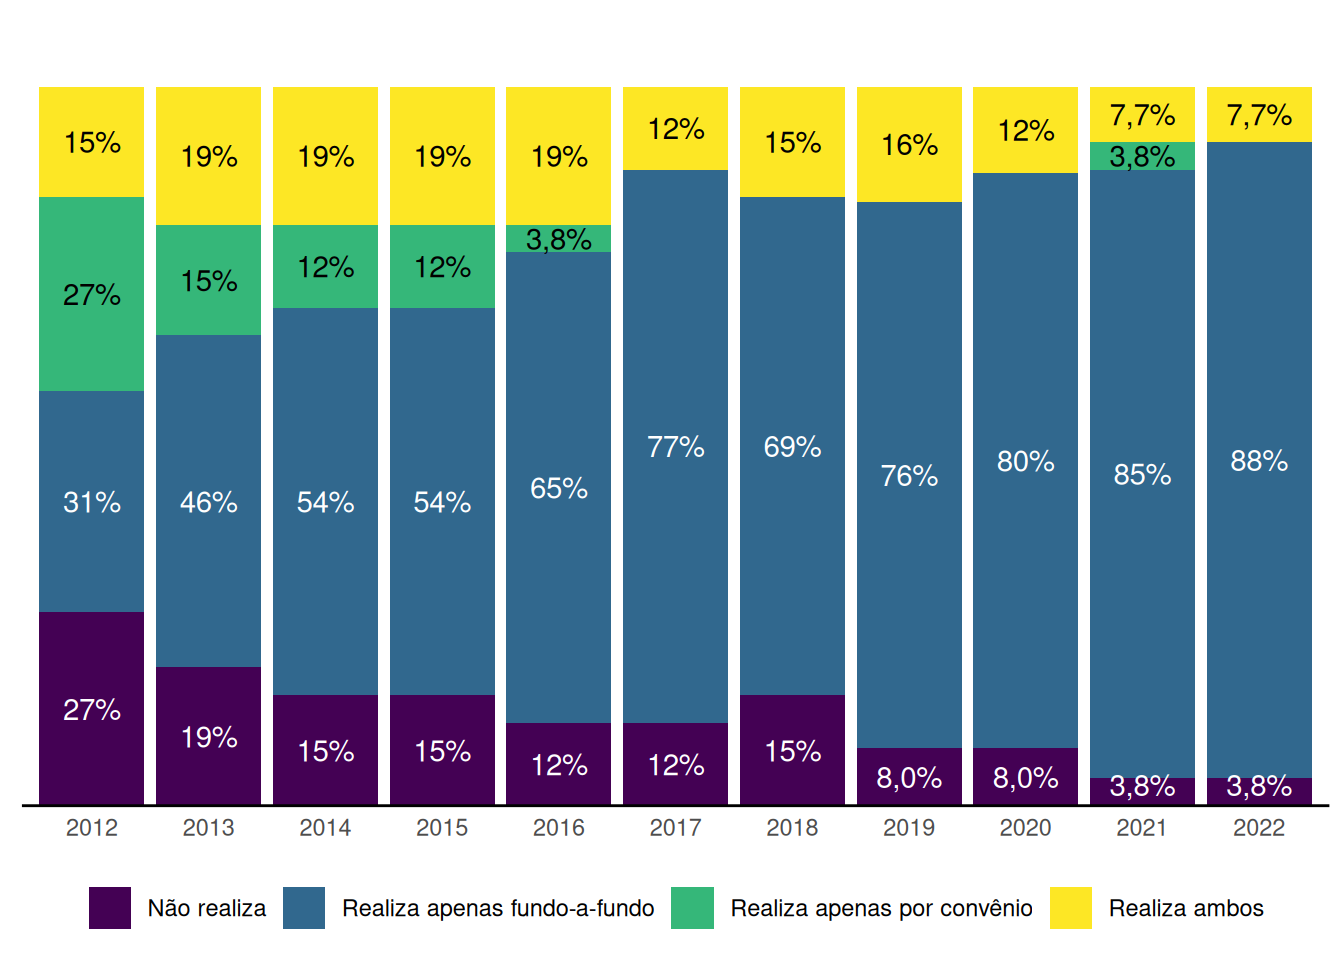
\includegraphics{gestao_files/figure-pdf/fig-estados-cofinanciamento-municipios-1.pdf}

}

\caption{\label{fig-estados-cofinanciamento-municipios}Percentual de
estados segundo realização de cofinanciamento aos municípios - Brasil;
2012 a 2022}

\end{figure}%

O Gráfico~\ref{fig-estados-blocos-recursos} evidencia a quantidade de
estados quando ao cofinanciamento aos municípios por blocos. Os dados
dos últimos 10 anos, sinaliza que o número de estados que cofinanciam os
municípios vem aumentando. Sobretudo o cofinanciamento da proteção
social especial (Média e Alta Complexidade), em seguida Benefícios
Eventuais. No que se refere aos últimos 5 anos houve uma redução na
destinação de recursos para proteção social básica e incentivos do SUAS.

\begin{figure}

\centering{

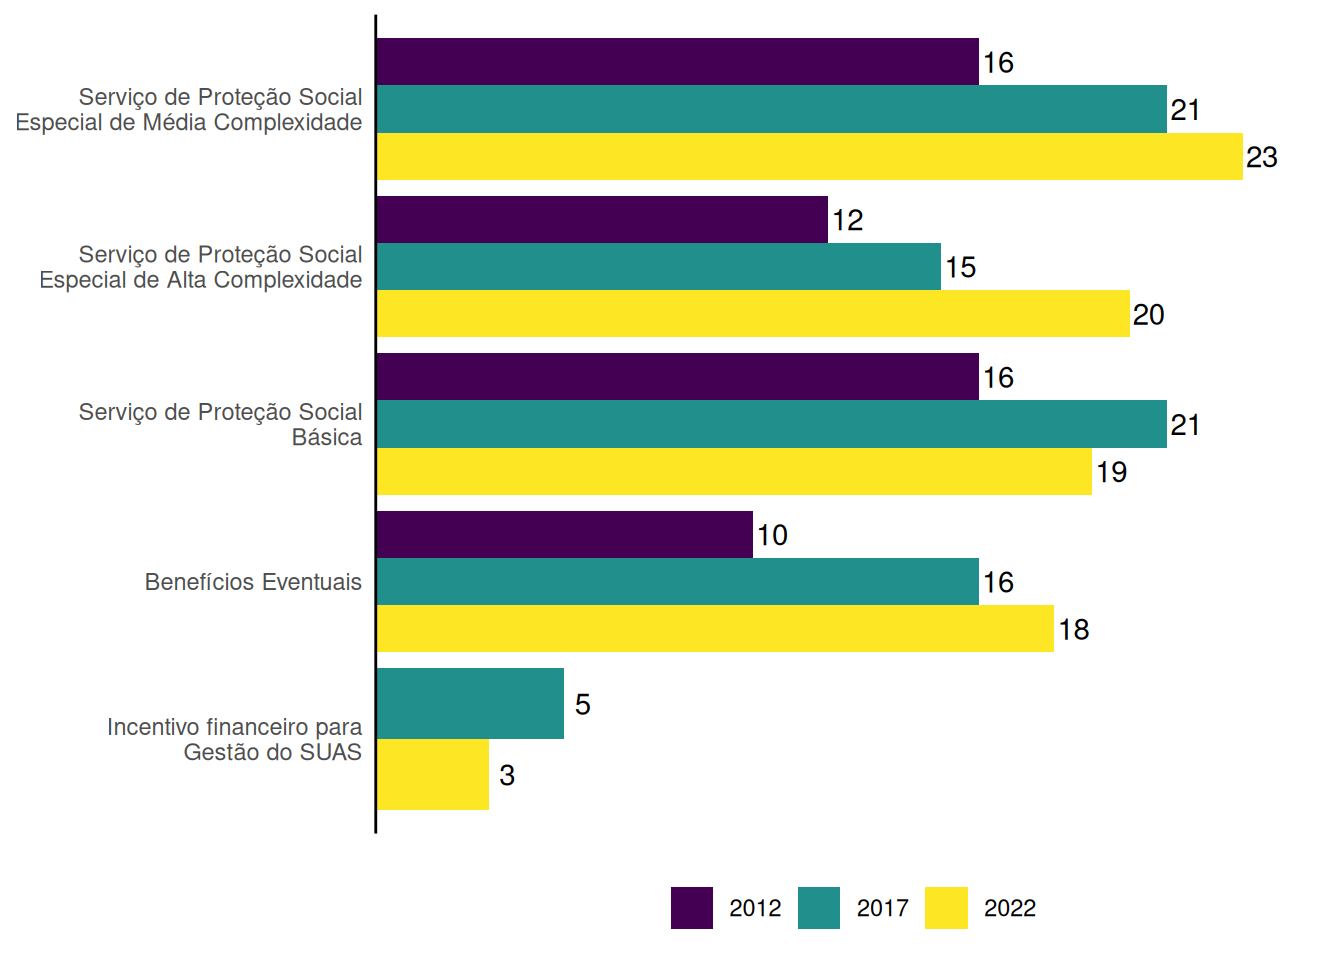
\includegraphics{gestao_files/figure-pdf/fig-estados-blocos-recursos-1.pdf}

}

\caption{\label{fig-estados-blocos-recursos}Número de estados segundo a
destinação dos recursos transferidos aos municípios por blocos de
financiamento - Brasil; 2012, 2017 e 2022}

\end{figure}%

O ordenador de despesa responde pela emissão de empenho, autorização de
pagamento dos recursos do fundo de assistência social. Assim,
recomenda-se que este tenha amplo conhecimento sobre a política. O
Gráfico~\ref{fig-estado_ord_despesa} sinaliza que 73\% dos gestores
estaduais são ordenadores de despesa do fundo estadual. Dado que reduziu
a partir de 2018.

\begin{figure}

\centering{

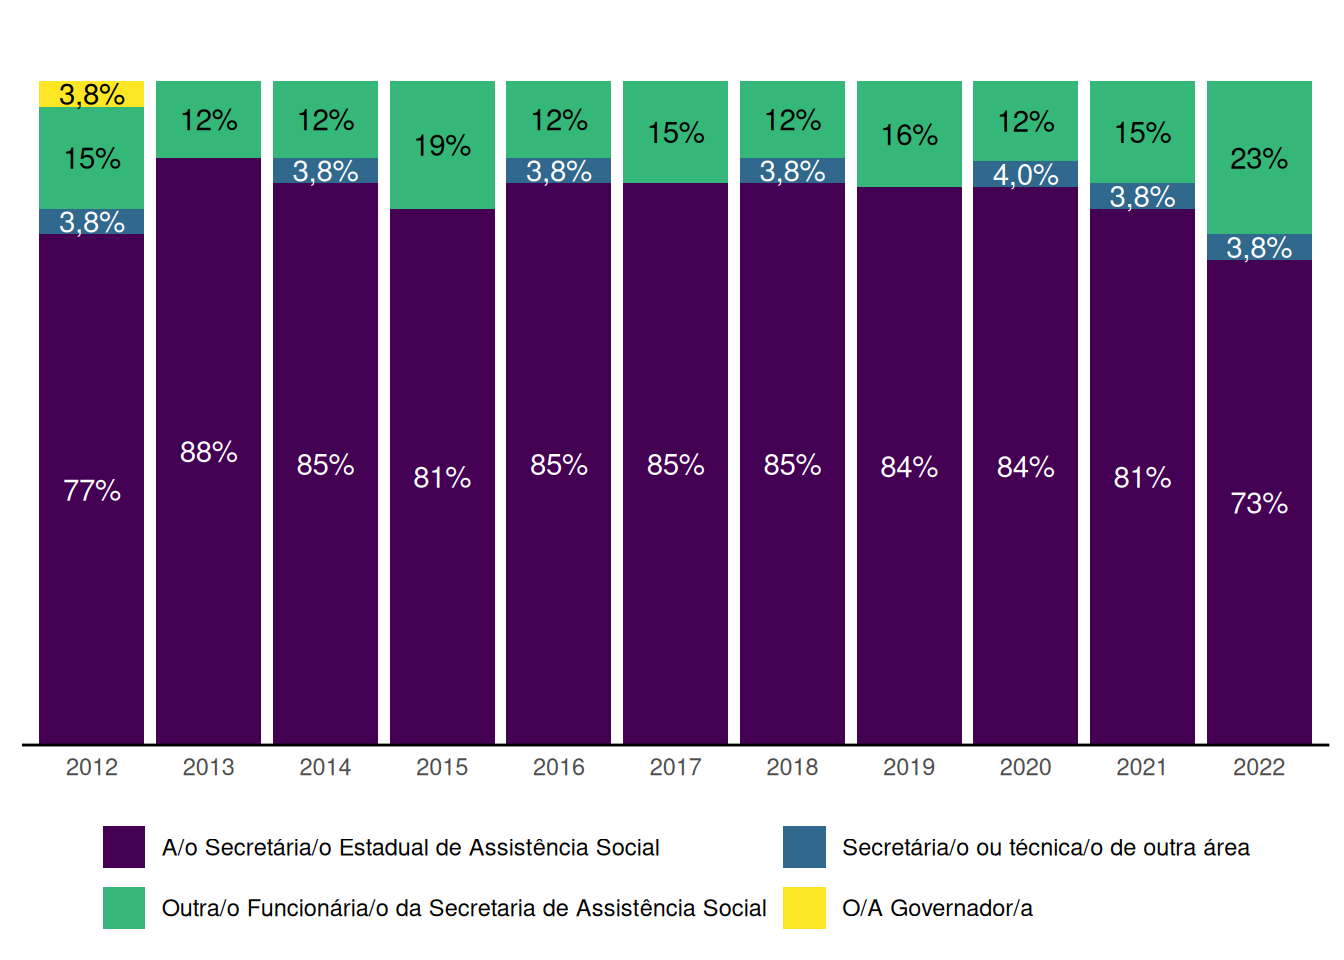
\includegraphics{gestao_files/figure-pdf/fig-estado_ord_despesa-1.pdf}

}

\caption{\label{fig-estado_ord_despesa}Percentual de estados quanto a
ordenação de despesa do Fundo Estadual - Brasil, 2018-2022}

\end{figure}%

No que se refere aos municípios, aproximadamente 80\% das/os
secretárias/os municipais são ordenadores de despesa do Fundo Municipal.
Esse percentual aumentou a partir de 2016.

O Gráfico~\ref{fig-munic_ord_despesa} também mostra que as/os
prefeitas/os enquanto ordenadores de despesa da política de Assistência
Social vem reduzindo ao longo dos anos. Dado que se revela como
positivo, haja vista o gestor municipal encontra-se no cotidiano do
planejamento desta política pública, sendo mais apropriado para tomar as
decisões sobre o orçamento.

\begin{figure}

\centering{

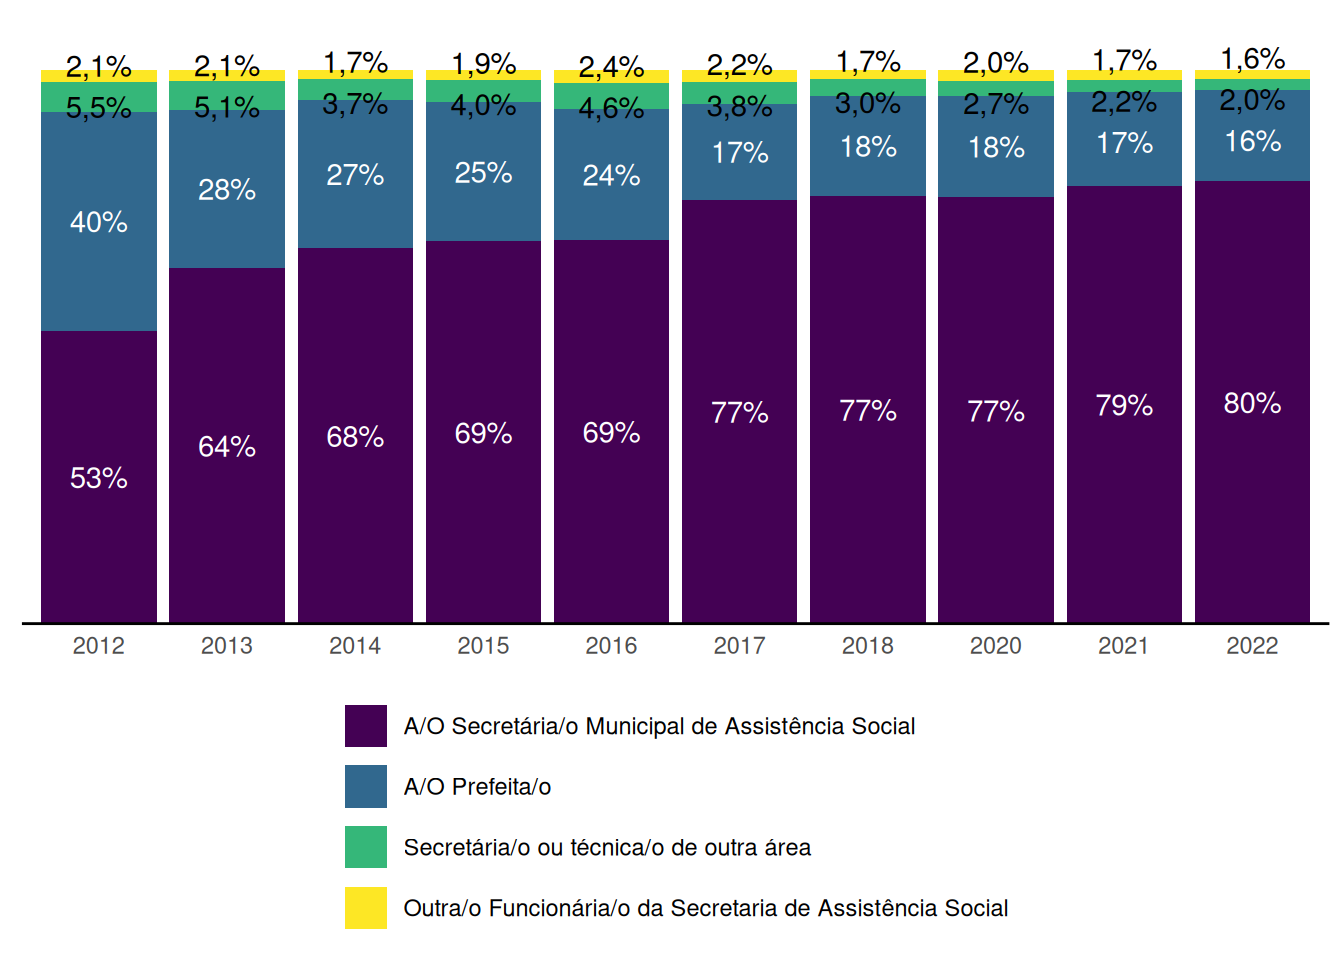
\includegraphics{gestao_files/figure-pdf/fig-munic_ord_despesa-1.pdf}

}

\caption{\label{fig-munic_ord_despesa}Percentual de municípios quanto a
ordenação de despesa do Fundo Municipal - Brasil, 2013 - 2022}

\end{figure}%

\section{Programas de execução própria executadas pelos
estados}\label{programas-de-execuuxe7uxe3o-pruxf3pria-executadas-pelos-estados}

Em relação aos programas próprios de transferência de renda executados
pelos estados, percebe-se um aumento ao longo dos anos na qual em 2022,
65\% dos estados informaram que possuem conforme o
Gráfico~\ref{fig-be_uf_renda}.

\begin{figure}

\centering{

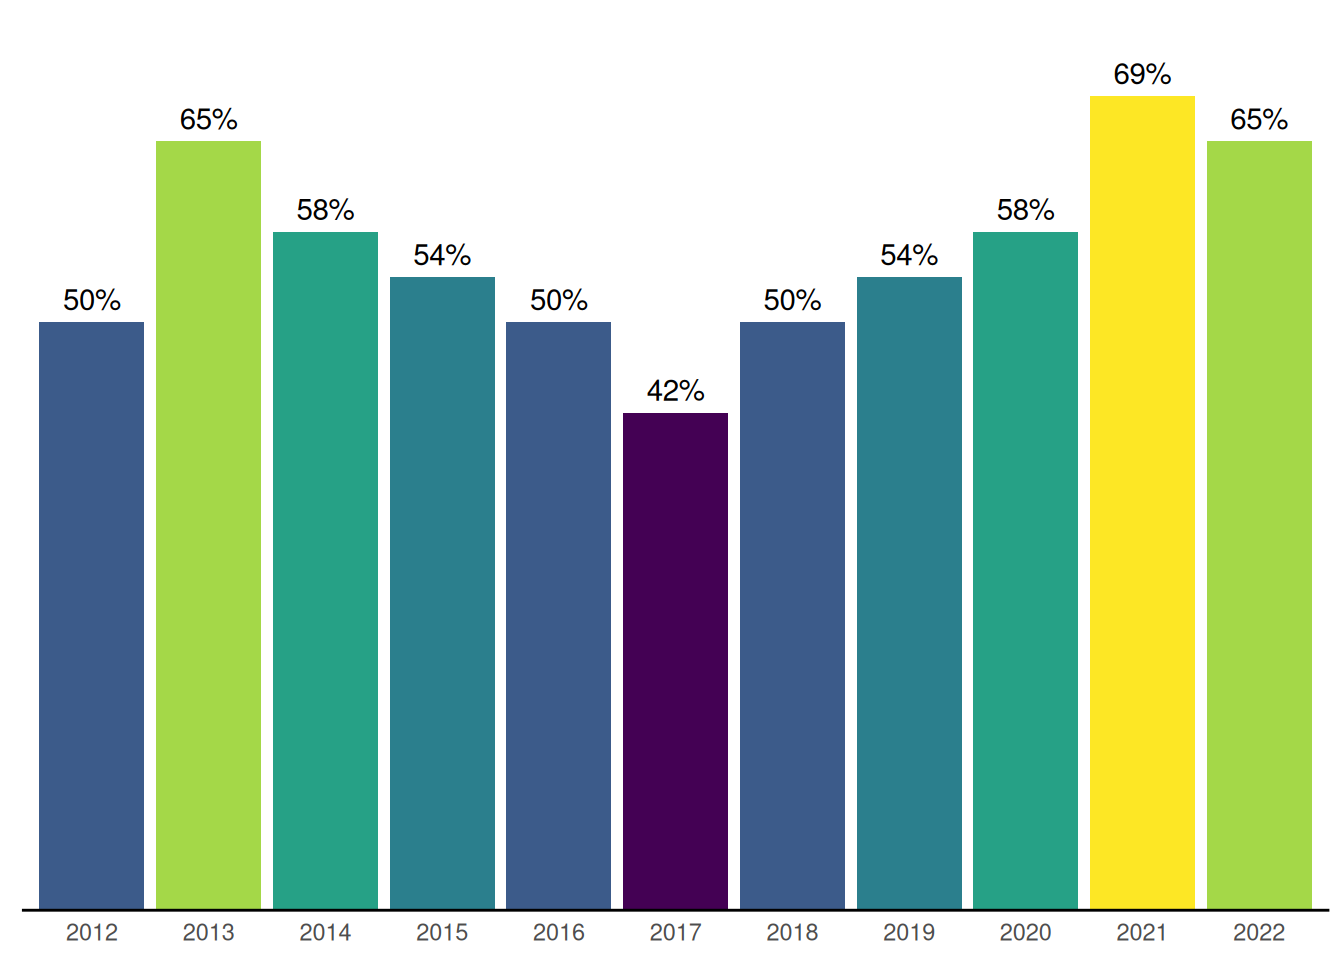
\includegraphics{gestao_files/figure-pdf/fig-be_uf_renda-1.pdf}

}

\caption{\label{fig-be_uf_renda}Percentual de estados que possuem
programa próprio de transferência de renda}

\end{figure}%

Destes estados (17) que informam possuir programa próprio de
transferência de renda, 82,3\% utilizam o Cadastro Único para seleção
das pessoas beneficiárias.

\section[Gestão do Cadastro Único]{\texorpdfstring{Gestão do Cadastro
Único\footnote{O formulário do posto do Cadastro Único foi criado em
  2020, assim a maioria das informações disponíveis terão referência a
  esta data.}}{Gestão do Cadastro Único}}\label{gestuxe3o-do-cadastro-uxfanico24}

O Cadastro Único para Programas Sociais do Governo Federal (Cadastro
Único) instituído por meio do art. 6º-F da Lei nº 8.742, de 7 de
dezembro de 1993 (Lei Orgânica da Assistência Social), e regulamentado
por meio do Decreto nº 11.016, de 29 de março de 2022 tem a finalidade
de coletar, sistematizar e disseminar informações que permitem a
identificação e caracterização das condições socioeconômicas das
famílias em situação de vulnerabilidade social, sobretudo para as
famílias de baixa de renda.

O objetivo é conhecer, incluir e aprimorar as políticas sociais através
do acesso a serviços, programas, benefícios, identificação das famílias
e territórios vulnerabilizados, bem como ações intersetoriais.

A gestão do Cadastro Único é compartilhada entre União, Estados,
Municípios e Distrito Federal na qual cabe aos estados o apoio técnico,
capacitação, monitoramento e avaliação. É nos municípios que estão os
locais de cadastramento e toda gestão territorial da identificação das
famílias neste cadastro público.

As unidades do Cadastro Único podem ser encontradas em locais exclusivos
ou na rede de atendimento socioassistencial de CRAS, CREAS, Centro POP.
Dados do Censo SUAS mostram uma evolução de locais de cadastramento,
sobretudo a partir de 2017.

Sobre a distribuição destes locais de Cadastro Único, destaca-se que em
2022, 31\% (2.892) são unidades exclusivas de Cadastro Único e 68\%
(6.435) estão em unidades da rede socioassistencial\footnote{CRAS, CREAS
  e CENTRO POP} conforme pode ser observado na tabela
Tabela~\ref{tbl-qtd_unidades}.

\begin{longtable}[]{@{}
  >{\raggedright\arraybackslash}p{(\columnwidth - 12\tabcolsep) * \real{0.2584}}
  >{\centering\arraybackslash}p{(\columnwidth - 12\tabcolsep) * \real{0.1236}}
  >{\centering\arraybackslash}p{(\columnwidth - 12\tabcolsep) * \real{0.1236}}
  >{\centering\arraybackslash}p{(\columnwidth - 12\tabcolsep) * \real{0.1236}}
  >{\centering\arraybackslash}p{(\columnwidth - 12\tabcolsep) * \real{0.1236}}
  >{\centering\arraybackslash}p{(\columnwidth - 12\tabcolsep) * \real{0.1236}}
  >{\centering\arraybackslash}p{(\columnwidth - 12\tabcolsep) * \real{0.1236}}@{}}
\caption{Quantidade de Unidades de Cadastro
Único}\label{tbl-qtd_unidades}\tabularnewline
\toprule\noalign{}
\begin{minipage}[b]{\linewidth}\raggedright
Unidades
\end{minipage} & \begin{minipage}[b]{\linewidth}\centering
2017
\end{minipage} & \begin{minipage}[b]{\linewidth}\centering
2018
\end{minipage} & \begin{minipage}[b]{\linewidth}\centering
2019
\end{minipage} & \begin{minipage}[b]{\linewidth}\centering
2020
\end{minipage} & \begin{minipage}[b]{\linewidth}\centering
2021
\end{minipage} & \begin{minipage}[b]{\linewidth}\centering
2022
\end{minipage} \\
\midrule\noalign{}
\endfirsthead
\toprule\noalign{}
\begin{minipage}[b]{\linewidth}\raggedright
Unidades
\end{minipage} & \begin{minipage}[b]{\linewidth}\centering
2017
\end{minipage} & \begin{minipage}[b]{\linewidth}\centering
2018
\end{minipage} & \begin{minipage}[b]{\linewidth}\centering
2019
\end{minipage} & \begin{minipage}[b]{\linewidth}\centering
2020
\end{minipage} & \begin{minipage}[b]{\linewidth}\centering
2021
\end{minipage} & \begin{minipage}[b]{\linewidth}\centering
2022
\end{minipage} \\
\midrule\noalign{}
\endhead
\bottomrule\noalign{}
\endlastfoot
CRAS & 5.669 & 5.508 & 5.923 & 5.729 & 5.937 & 6.090 \\
CREAS & 281 & 174 & 199 & 199 & 208 & 230 \\
Centro POP & 112 & 83 & 84 & 108 & 106 & 115 \\
Postos Cadastro Único & - & - & - & 2.530 & 2.695 & 2.892 \\
\textbf{Total} & \textbf{6.062} & \textbf{5.765} & \textbf{6.206} &
\textbf{8.566} & \textbf{8.946} & \textbf{9.327} \\
\end{longtable}

A respeito da estrutura física das unidades exclusivas do Cadastro Único
destacadas acima, 61,0\% encontram-se na sede da Secretaria de
Assistência Social e 24,3\% em estruturas específicas. Os demais
percentuais são encontrados em outra unidade administrativa como, em um
serviço integrado, OSC´s, conselho ou escola.

No que se refere a gestão territorial, cabe as coordenações do Cadastro
Único dos municípios o atendimento, a supervisão, o monitoramento e a
avaliação dos processos de cadastramento, seja em postos específicos ou
integradas as unidades da rede socioassistencial.

O Gráfico~\ref{fig-gestao_cad} sinaliza que, no âmbito da gestão
municipal, as ações de levantamento de famílias para atualização e
inclusão cadastral são a mais realizada. A menor proporção se refere a
ações de elaboração de análises utilizando dados do Cadastro Único
(Gráfico~\ref{fig-gestao_cad})\footnote{estas informações são do
  formulário de Gestão Municipal, assim se referem a informações gerais
  que a gestão informa realizar, destaca-se também que estas informações
  estão disponíveis a partir do ano de 2020 entretanto, só foi possível
  gerar a partir de 2021 em decorrência de problemas na leitura da base}.

\begin{figure}

\centering{

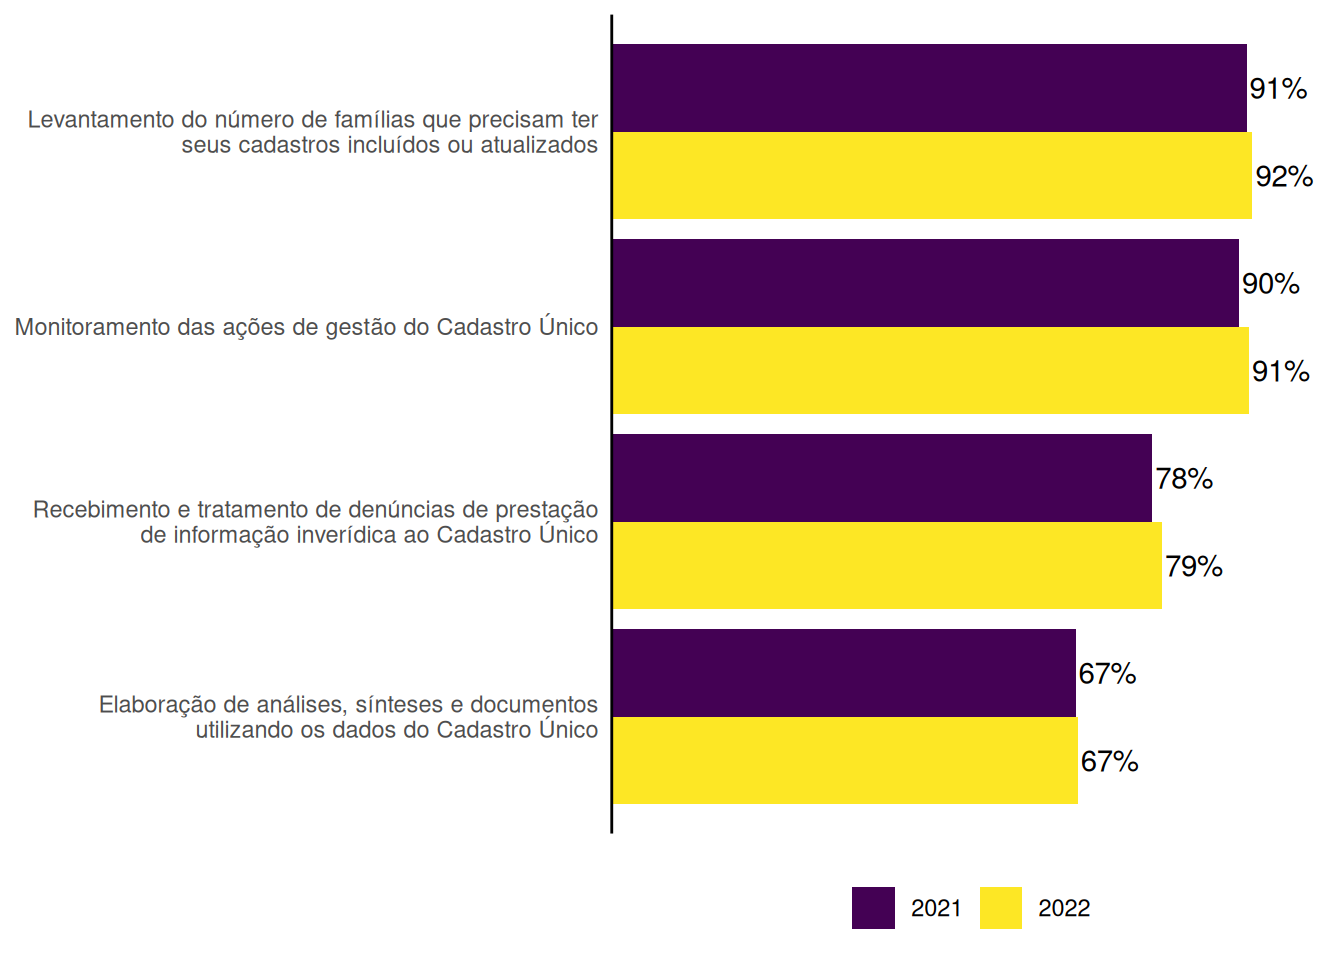
\includegraphics{gestao_files/figure-pdf/fig-gestao_cad-1.pdf}

}

\caption{\label{fig-gestao_cad}Ações desenvolvidas no âmbito da Gestão
do Cadastro Único - Brasil, 2021 e 2022}

\end{figure}%

O Gráfico~\ref{fig-acoes_cad} sinaliza que as ações de esclarecimento de
dúvidas sobre serviços, programas entre outros são realizadas pela
grande maioria das unidades do Cadastro Único (96,82\%). Já as ações de
agendamento para atendimento são realizadas por 64,35\% das unidades,
com redução ao longo dos anos\footnote{estas informações são dos postos
  que executam exclusivamente atividades do Cadastro Único}.

\begin{figure}

\centering{

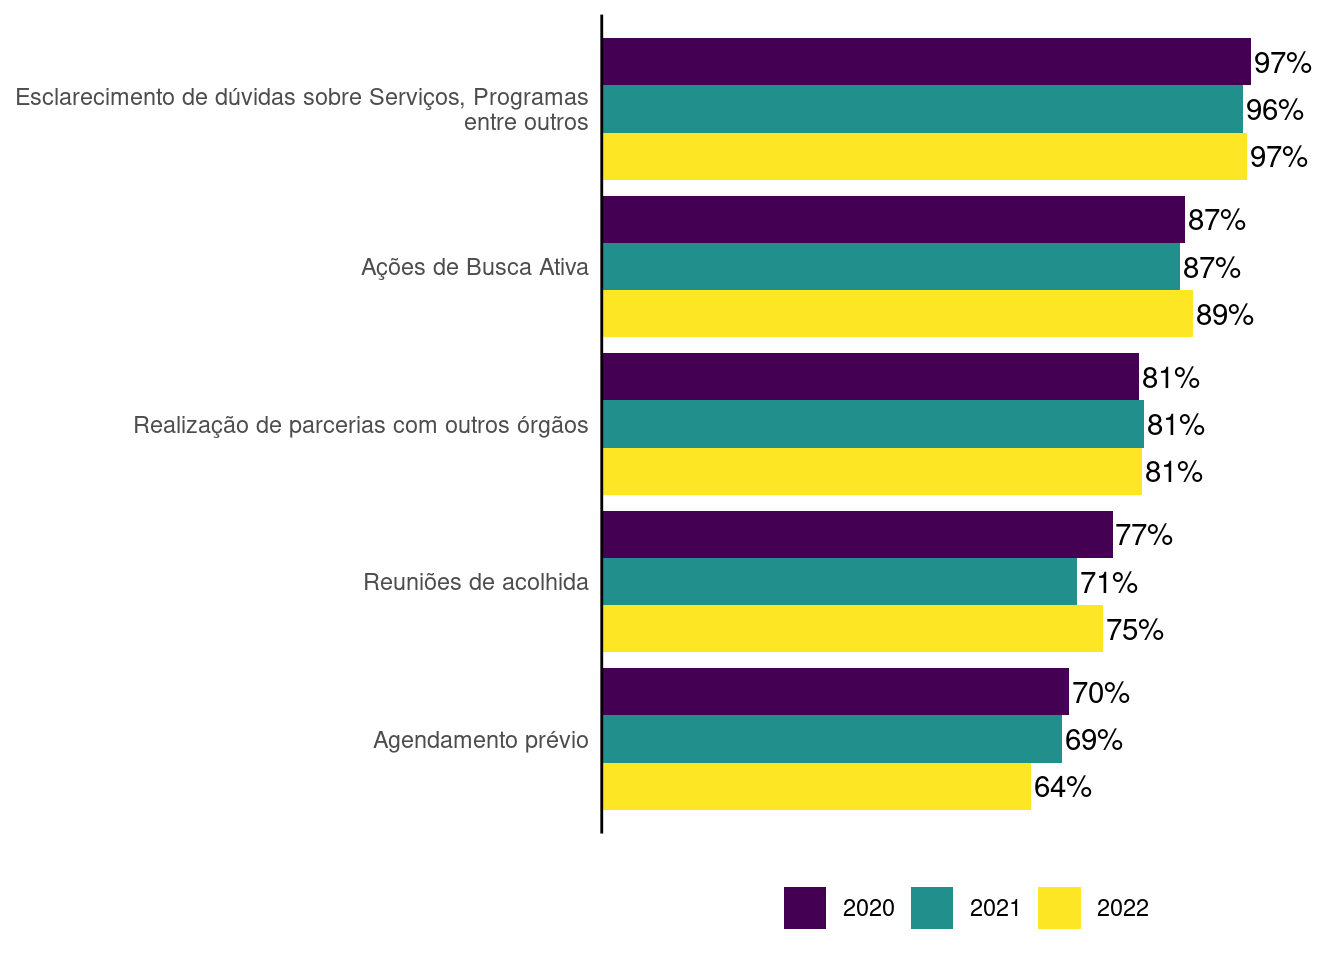
\includegraphics{gestao_files/figure-pdf/fig-acoes_cad-1.pdf}

}

\caption{\label{fig-acoes_cad}Ações desenvolvidas pelos postos do
Cadastro Único - Brasil, 2020, 2021 e 2022}

\end{figure}%

Faz parte de procedimentos de qualificação do Cadastro Único ações de
averiguação e revisão cadastral. A averiguação é um processo de
verificação das informações registradas no Cadastro Único por meio da
comparação dos dados declarados pelas famílias com outros dados e
registros administrativos do governo federal. Já a revisão é um
procedimento de atualização das famílias com registros desatualizados. O
tempo considerado para um cadastro desatualizado é de 24 meses. O
Gráfico~\ref{fig-ave_cad} refere-se as informações de averiguação e
revisão cadastral no âmbito dos postos dos Cadastro Único dos
municípios. Nota-se que ao longo dos anos, essas ações
aumentaram,sobretudo as ações de busca ativa e identificação do público
de averiguação e revisão cadastral como público prioritário.

\begin{figure}

\centering{

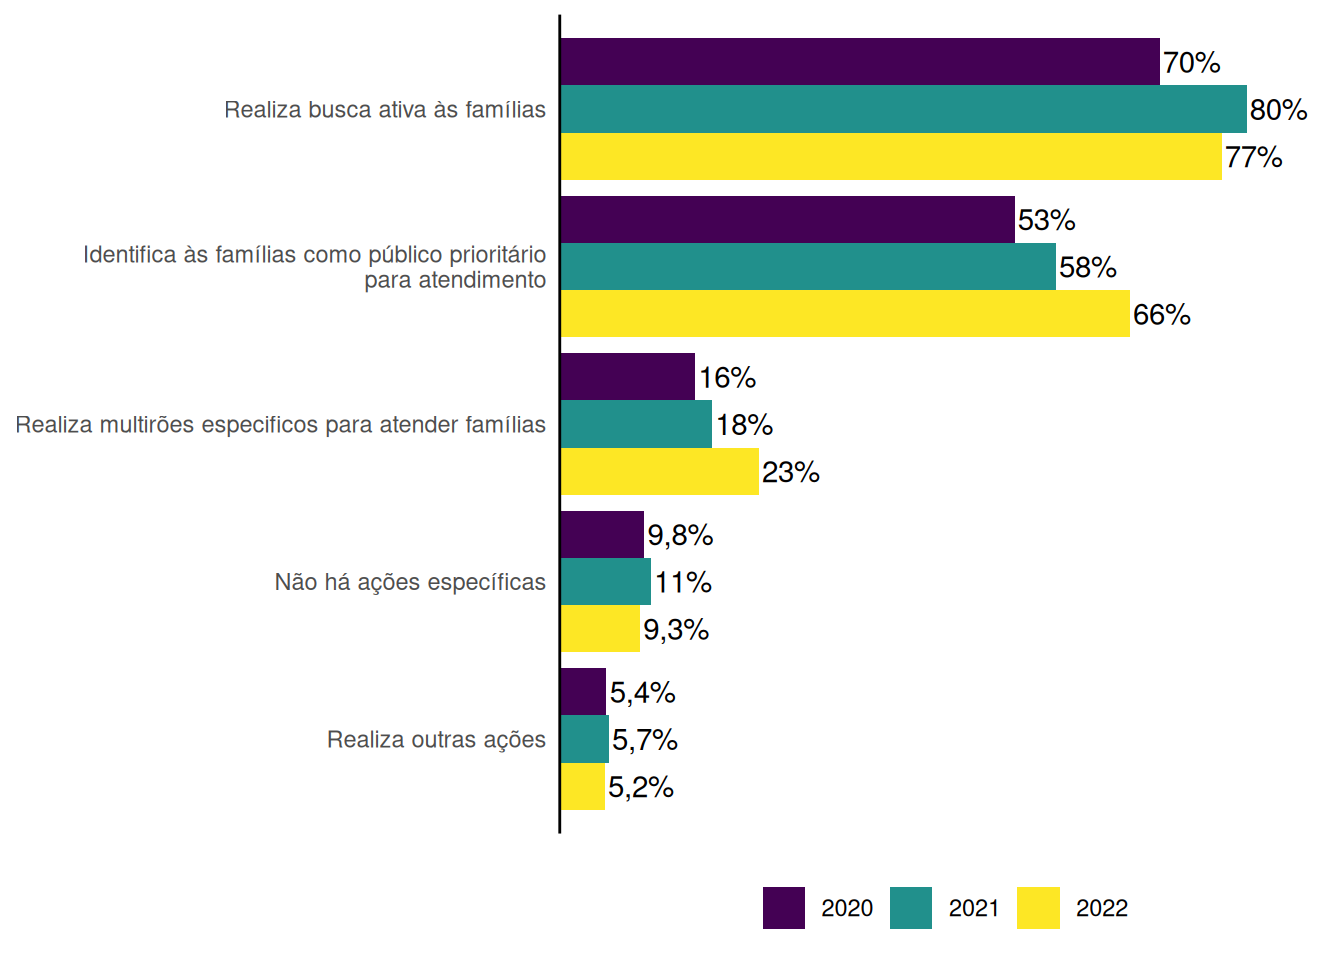
\includegraphics{gestao_files/figure-pdf/fig-ave_cad-1.pdf}

}

\caption{\label{fig-ave_cad}Ações de averiguação e revisão desenvolvidas
pelas Unidades do Cadastro Único - Brasil, 2020, 2021 e 2022}

\end{figure}%

Em relação as informações de unidades de Postos do Cadasto Único e o
atendimento de Grupos Populacionais Tradicionais e Específicos - GPTEs,
destaca-se através do Gráfico~\ref{fig-gptes-cadunico} o percentual de
unidades de postos do Cadastro Único que informam atender no período de
2020 a 2022.

\begin{figure}

\centering{

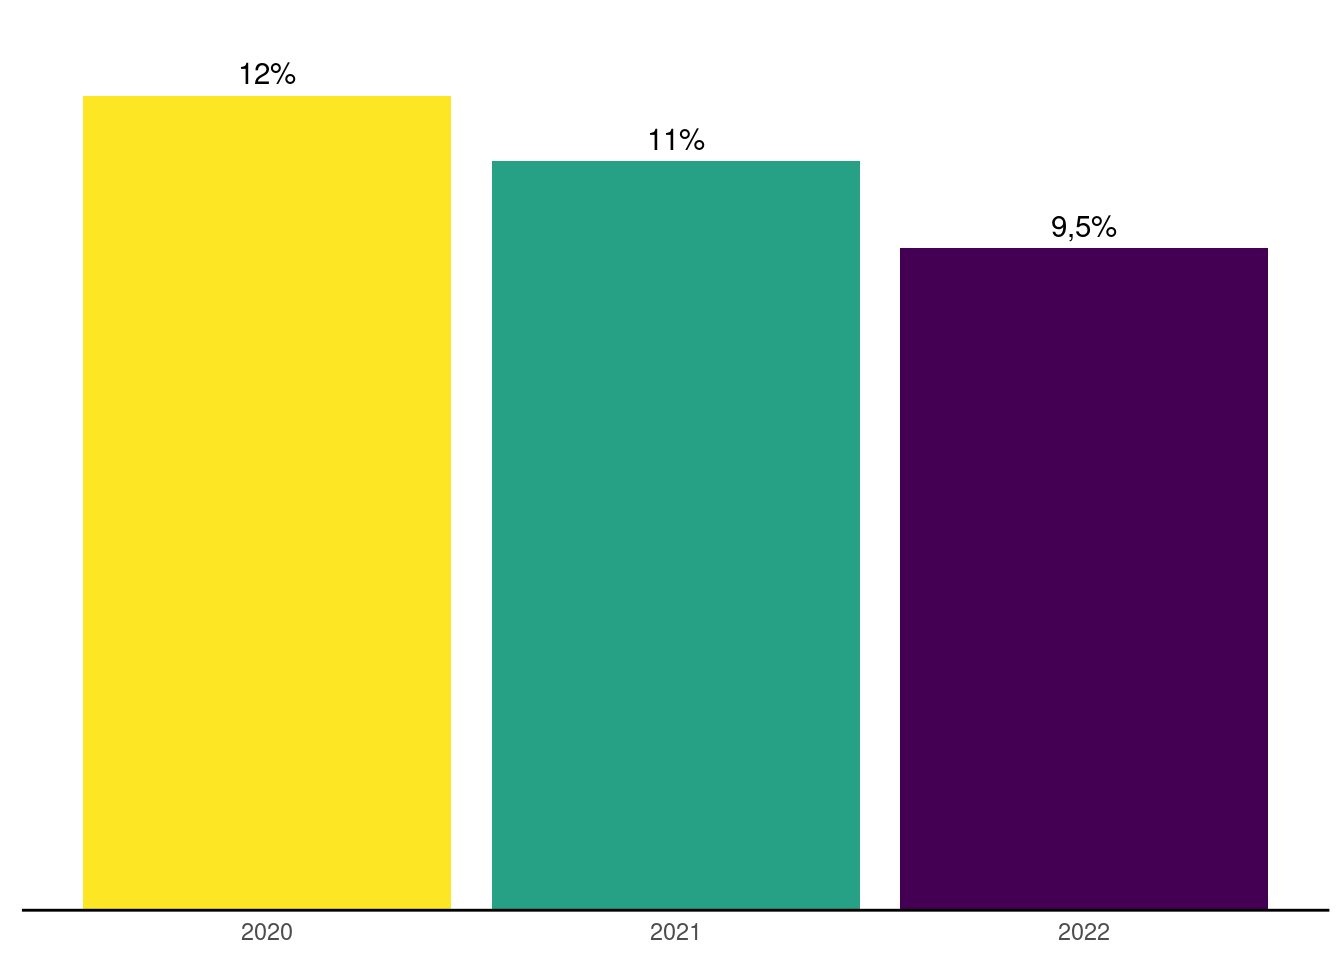
\includegraphics{gestao_files/figure-pdf/fig-gptes-cadunico-1.pdf}

}

\caption{\label{fig-gptes-cadunico}Unidades que realizam cadastramento
de famílias pertencentes a Grupos Tradicionais e Específicos (GPTEs) -
Brasil, 2020 a 2022}

\end{figure}%

O cadastramento domiciliar permite uma aproximação com aspectos do
cotidiano das famílias, visto que a coleta das informações ocorre por
meio do encontro da gestão até as famílias. Essa ação objetiva assegurar
o acesso a inclusão ou atualização cadastral na residência das pessoas.
De acordo com informações do Gráfico~\ref{fig-visit_dom} as situações
mais frequentes para visita domiciliar são para averiguação cadastral e
inclusão/atualização de dados do BPC (Benefício de Prestação Continuada
- BPC).

\begin{figure}

\centering{

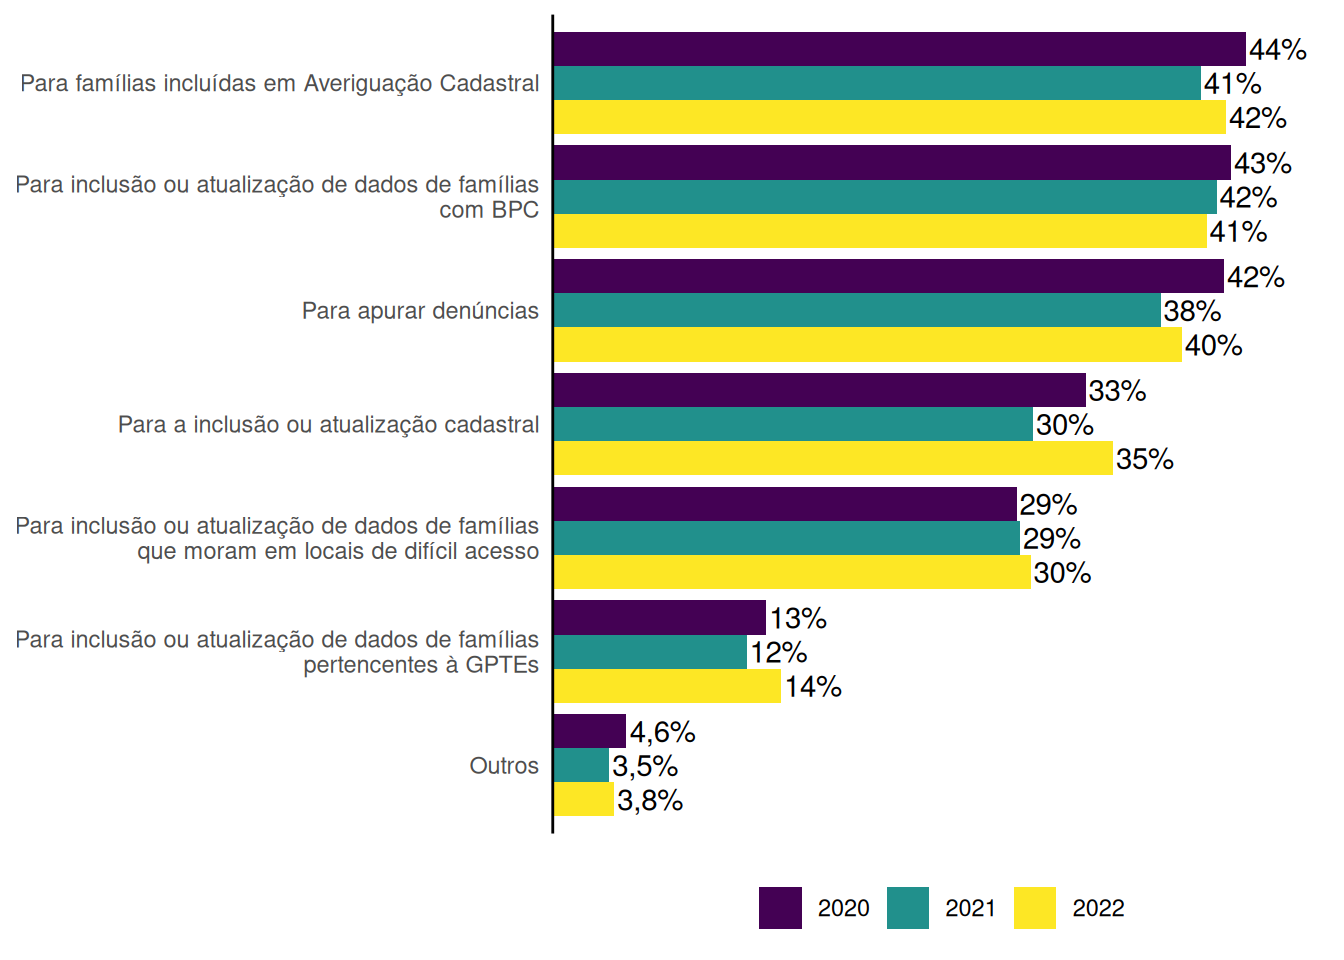
\includegraphics{gestao_files/figure-pdf/fig-visit_dom-1.pdf}

}

\caption{\label{fig-visit_dom}Situações mais frequentes de entrevistas
domiciliares no Cadastro Único - Brasil, 2020, 2021 e 2022}

\end{figure}%

Em relação as ações de complementariedade com a rede socioassistencial,
destaca-se que a maioria destas unidades de cadastramento realizam
encaminhamentos para rede socioassistencial de CRAS, CREAS, Centro POP
entre outros (Gráfico~\ref{fig-redesuas}).

\begin{figure}

\centering{

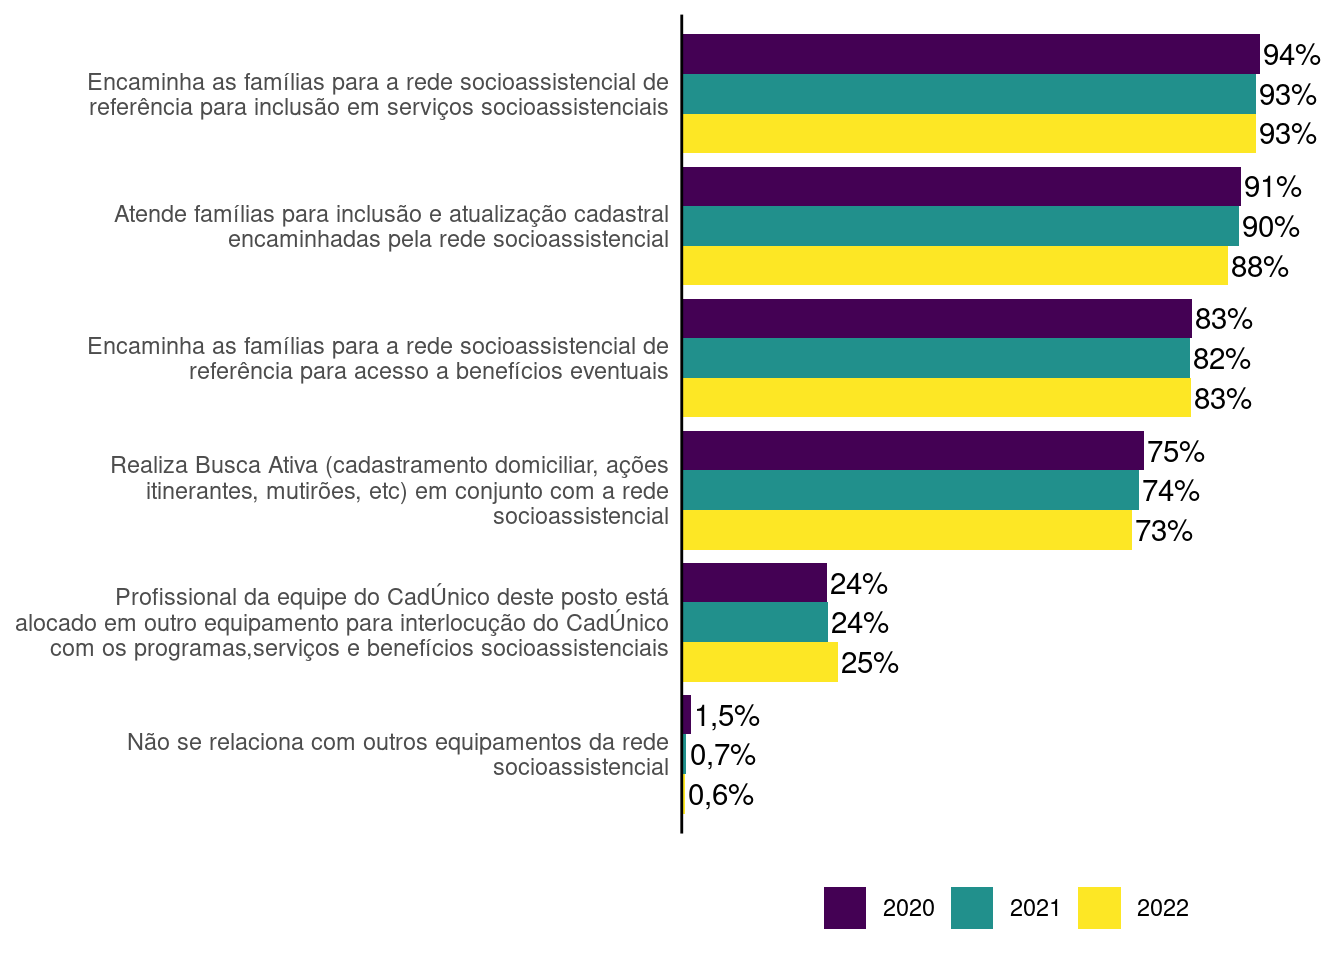
\includegraphics{gestao_files/figure-pdf/fig-redesuas-1.pdf}

}

\caption{\label{fig-redesuas}Percentual de postos de Cadastro Único
segundo relação com os outros equipamentos da rede socioassistencial -
Brasil, 2020, 2021 e 2022}

\end{figure}%

O Gráfico~\ref{fig-igdbolsa} sinaliza sobre a existência da participação
das unidades do Cadastro único no planejamento dos recursos recebidos no
âmbito do IGD-PBF (Índice de Gestão Descentralizada da Gestão do Bolsa
Família e Cadastro Único).

Trata-se de um recurso repassado aos estados e municípios para apoio a
gestão do Cadastro Único e Bolsa Família. Esta informação é referente a
respostas do formulário dos postos de cadastramento em âmbito dos
municípios.

\begin{figure}

\centering{

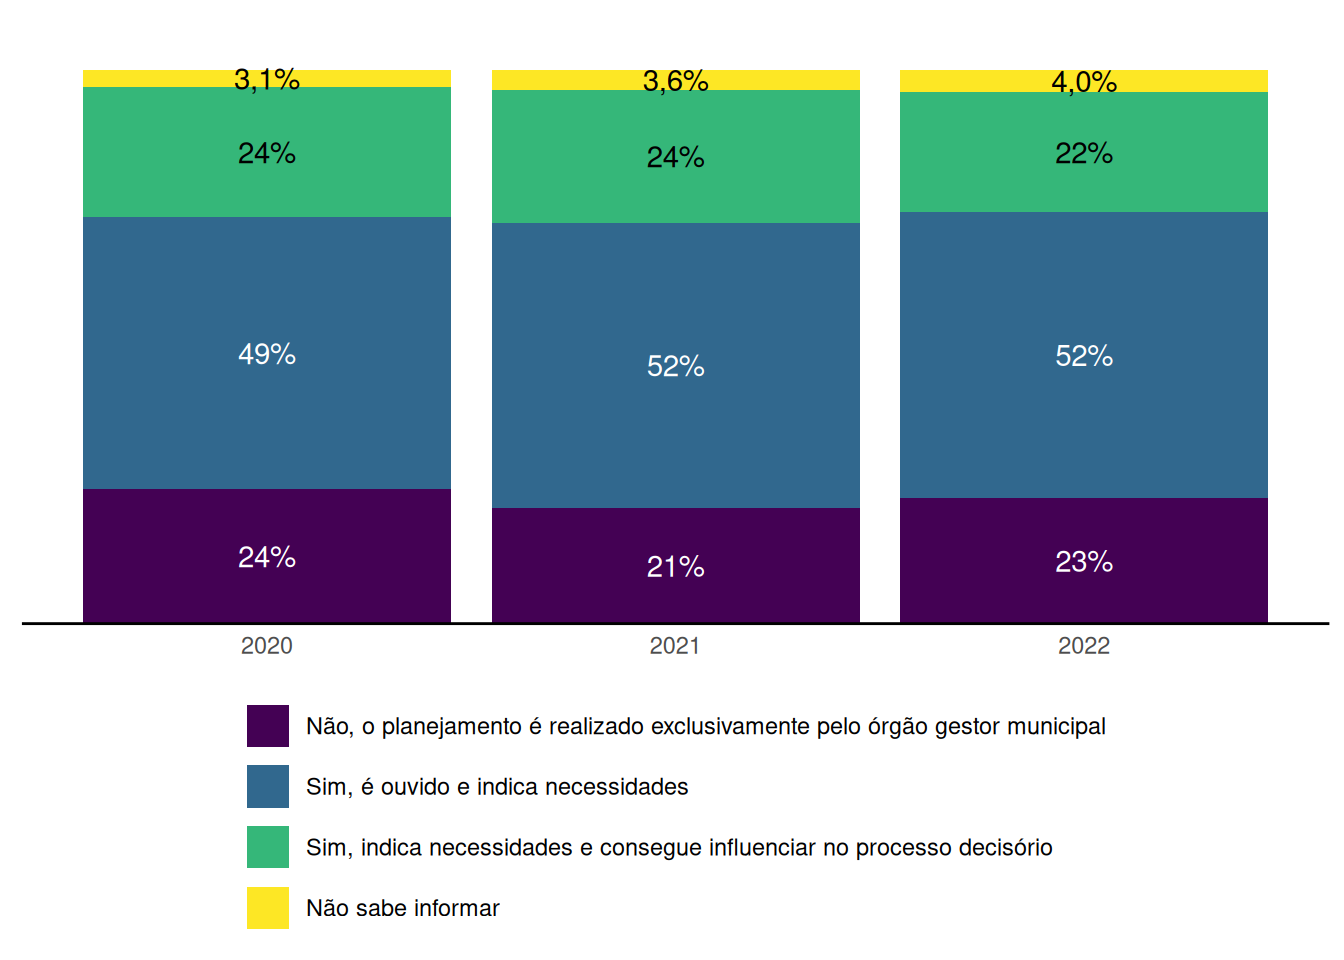
\includegraphics{gestao_files/figure-pdf/fig-igdbolsa-1.pdf}

}

\caption{\label{fig-igdbolsa}Unidades de Postos do Cadastro Único quanto
a participação no planejamento do IGD Bolsa Família - Brasil, 2020 -
2021 - 2022}

\end{figure}%

\section{Considerações Finais}\label{considerauxe7uxf5es-finais}

A Assistência Social é uma política de previsibilidade constitucional
reafirmadas por lei, normas, decretos, pactos. Assim, faz-se essencial
padrões de gestão e comandos únicos em todos os entes federados. Os
dados históricos sinalizam avanços e desafios para gestão do SUAS.

Os órgãos gestores da assistência social, tanto estaduais quanto
municipais, são estruturas fundamentais para a execução desta política.
O significado do direito caminham junto com o planejamento, ofertas
continuadas, padrões de respostas, comandos únicos etc.

Assim, para consolidação desta política que faz-se universal nos
territórios, é fundamental em todos entes federados estruturas
administrativas indicadas nos pactos, Lei compatível com LOAS, conforme
deliberação das conferências nacionais, comando único do gestor da pasta
entre outros.

Os dados sinalizam avanços, a respeito das subdivisões administrativas
que apresentavam maior percentual de formalização nos órgãos gestores
estaduais em 88,5\% dos estados. As que apresentavam menores percentuais
de formalização nos órgãos gestores estaduais eram as de Regulação do
SUAS (38,5\%) e de Gestão do Trabalho (57,7\%). Nos municípios,
destaca-se forte presença de formalização das gestões do Cadastro Único
e Bolsa Família, bem como a proteção social básica, com 80,68\% e
77,90\% respectivamente.

Os recursos recebidos via transação fundo-a-fundo, garantem maior
qualidade na distribuição, já que estes são fiscalizados pelos órgãos de
controle social e passam pelo crivo das Comissões Intergestores
Bipartite e Tripartite. Sobre o repasse, destacam-se o avanço ao longo
dos anos nesta forma repasse aliado ao cofinanciamento, sendo mais
presente o cofinancimento a Proteção Social Especial.

Aspectos relacionados a Gestão do Cadastro Único foi incorporada nesta
versão do Censo SUAS 2022, o objetivo é afirmar a importância deste
instrumento do SUAS. O Cadastro Único é uma ferramenta que visa
potencializar as funções de proteção social, vigilância socioassitencial
e defesa de direitos, Para isso, os dados promovem acesso a serviços e
programas, identificação das famílias e leitura dos territórios, bem
como parcerias e ações intersetoriais.

Destaca-se que do total de unidades de postos do Cadastro Único, 68\%
estão na rede socioassistencial e 31\% em postos exclusivos. Sobre estas
unidades, identifica-se que mais realizadas são Levantamento do número
de famílias que precisam ter seus cadastros incluídos ou atualizados e,
a menos desenvolvida é Elaboração de análises, sínteses e documentos
utilizando os dados do Cadastro Único.

Em relação aos posto exclusivos do Cadastro Único, as informações
sinalizam que 93\% destas unidades encaminham famílias para rede
socioassistecial, bem como 88\% recebem os encaminhamentos desta rede.
Enquanto desafios, destaca-se a importância da participação dos
profissionais das unidades de postos do Cadastro Único no planejamento
do IGD Bolsa Família. Os dados Censo SUAS 2022 sinaliza que 23\% deste
planejamento é realizado apenas pelo órgão gestor.

\bookmarksetup{startatroot}

\chapter{Unidades do SUAS}\label{unidades-do-suas}

Essa seção apresenta informações sobre as unidades físicas do SUAS e sua
evolução ao longo do tempo. Esse item contempla as seguintes
informações: a) quantidade de unidades administrativas da rede
socioassistencial, b) informações sobre acessibilidade, c) situação do
imovél e d) disponibilidade de equipamentos, como computador com acesso
à internet.

\section{Centros de Referência de Assistência Social
(CRAS)}\label{centros-de-referuxeancia-de-assistuxeancia-social-cras}

Os Centros de Referência de Assistência Social (CRAS) são definidos pelo
artigo 6º-C da Lei Orgânica de Assistência Social (LOAS) como unidades
públicas municipais destinadas à prestação de serviços, programas de
projetos da proteção social básica às famílias, devendo se localizar em
áreas com maiores índices de vulnerabilidade e risco social.

No Censo SUAS de 2022 foram identificados 8.557 CRAS, em 5.535
municípios brasileiros, o que indica que há pelo menos um CRAS em 99,4\%
dos municípios brasileiros.

O quantitativo de CRAS dobrou entre 2007 e 2022, passando de 4.195
unidades para 8.557. O Gráfico~\ref{fig-quantitativo-CRAS} apresenta a
evolução da quantidade de CRAS por grandes regiões de desenvolvimento.

\begin{figure}

\centering{

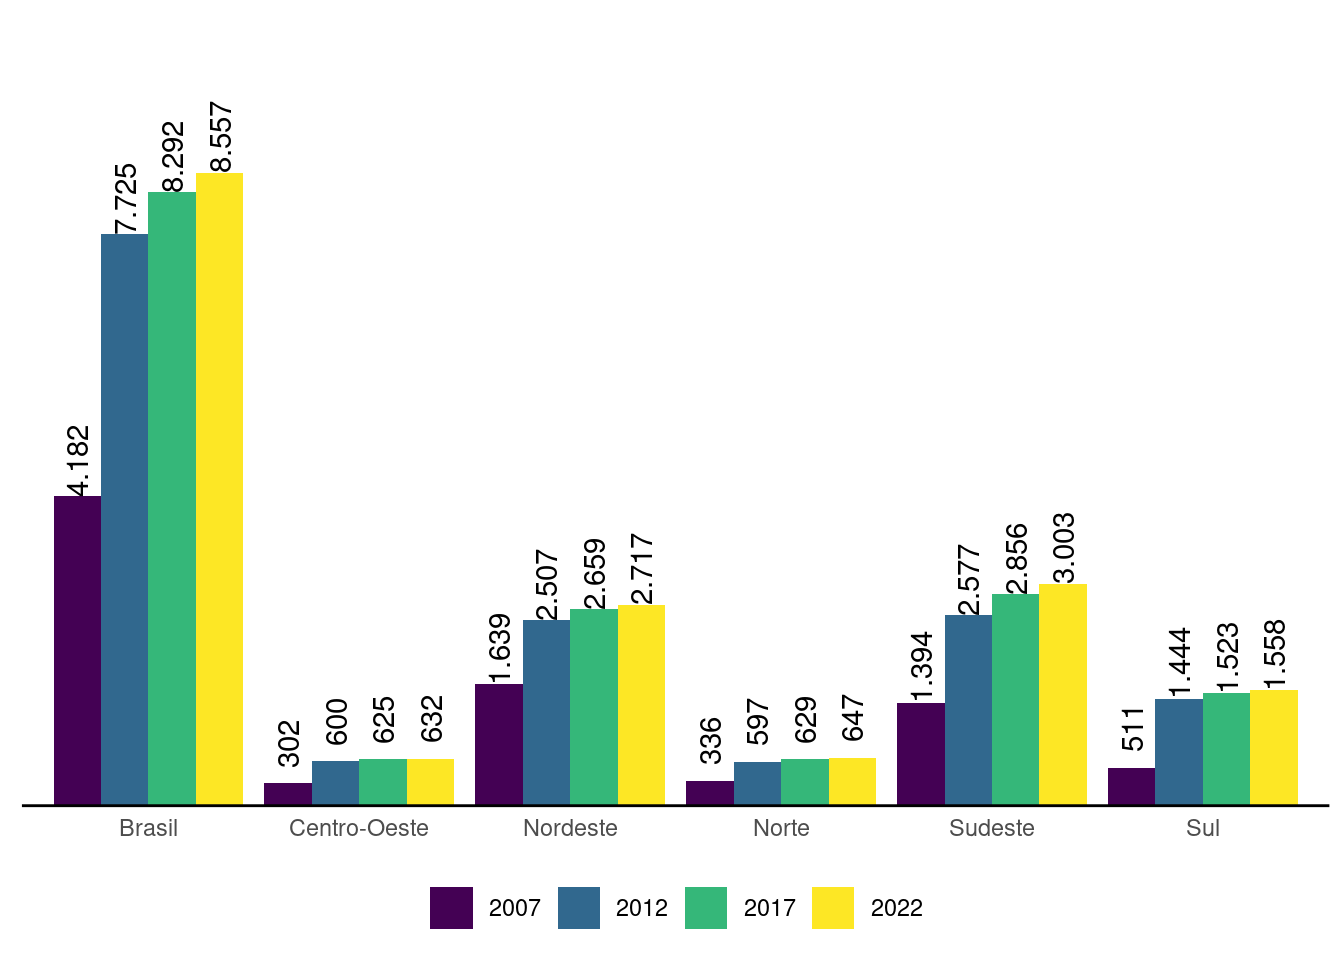
\includegraphics{unidades_files/figure-pdf/fig-quantitativo-CRAS-1.pdf}

}

\caption{\label{fig-quantitativo-CRAS}Evolução do quantitativo de CRAS,
segundo grandes regiões; 2007, 2012, 2017 e 2022}

\end{figure}%

A Expansão em todo território nacional do número de CRAS evidencia a
consolidação de uma referência de unidades públicas de Assistência
Social em todo território nacional. De acordo com os dados, 99,37\%
municípios possuem CRAS, ou seja, apenas 34 municípios no Brasil não
dispõem desta unidade pública\footnote{estas informações são referentes
  ao preenchimento do Censo SUAS, é possível que no determinado período
  esta unidade pública não tenha preenchido o forumulário}.

Ao observar o número de CRAS por municípios, levando-se em conta o porte
populacional, verifica-se que os 35 municípios do país que não possuem
CRAS\footnote{é possível também que alguns deles não tenham respondido
  ao Censo SUAS} e estão concentrados em municípios de pequeno porte
(Gráfico~\ref{fig-CRAS-porte}).

Em relação a concentração da quantidade de CRAS, para os municípios de
pequeno porte I e pequeno porte II, dispõem, em sua maioria, de uma
unidade de CRAS como referência do território, sendo respectivamente
96\% e 69\%. Os municípios de médio porte, cerca de 66\% possuem de 2 a
3 CRAS. Os municípios de grande porte, o grupo majoritário de unidades
são entre 4 a 6 CRAS - 52,5\%.

\begin{figure}

\centering{

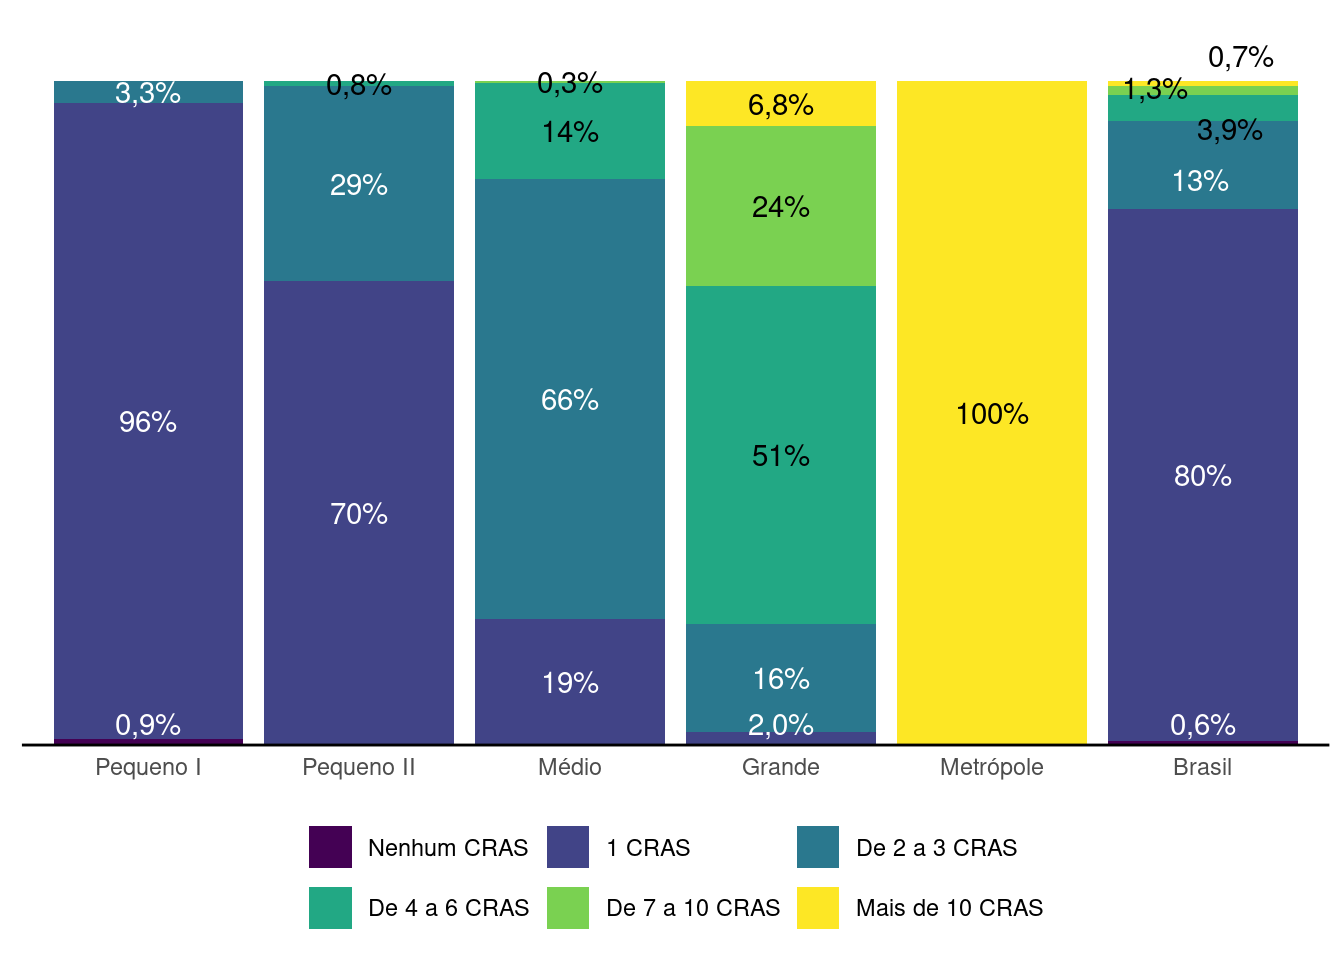
\includegraphics{unidades_files/figure-pdf/fig-CRAS-porte-1.pdf}

}

\caption{\label{fig-CRAS-porte}Percentual de municípios por número de
CRAS no município, segundo porte populacional estimado do município -
Brasil, 2022}

\end{figure}%

Os dados de CRAS que funcionam com imóvel próprio evoluiu
significativamente de 2008 a 2022. Destaca-se que o primeiro ano da
série histórica possuia 43,7\% CRAS com imóvel próprio
(Gráfico~\ref{fig-CRAS-imovel}), dado que chega em 2022 com 59,62\%.
Dados com CRAS que funcionam com imóveis alugados passam por redução de
48,2\% para 32,2\%.

Observa-se ainda aumento no percentual de CRAS que funcionam em imóveis
cedidos: eram 6,8\% em 2008, o maior valor da série histórica chega a
9,1\%, conforme mostra o Gráfico~\ref{fig-CRAS-imovel}.\footnote{Para os
  anos de 2018 e 2019 esse dado não foi coletado no Censo SUAS}

\begin{figure}

\centering{

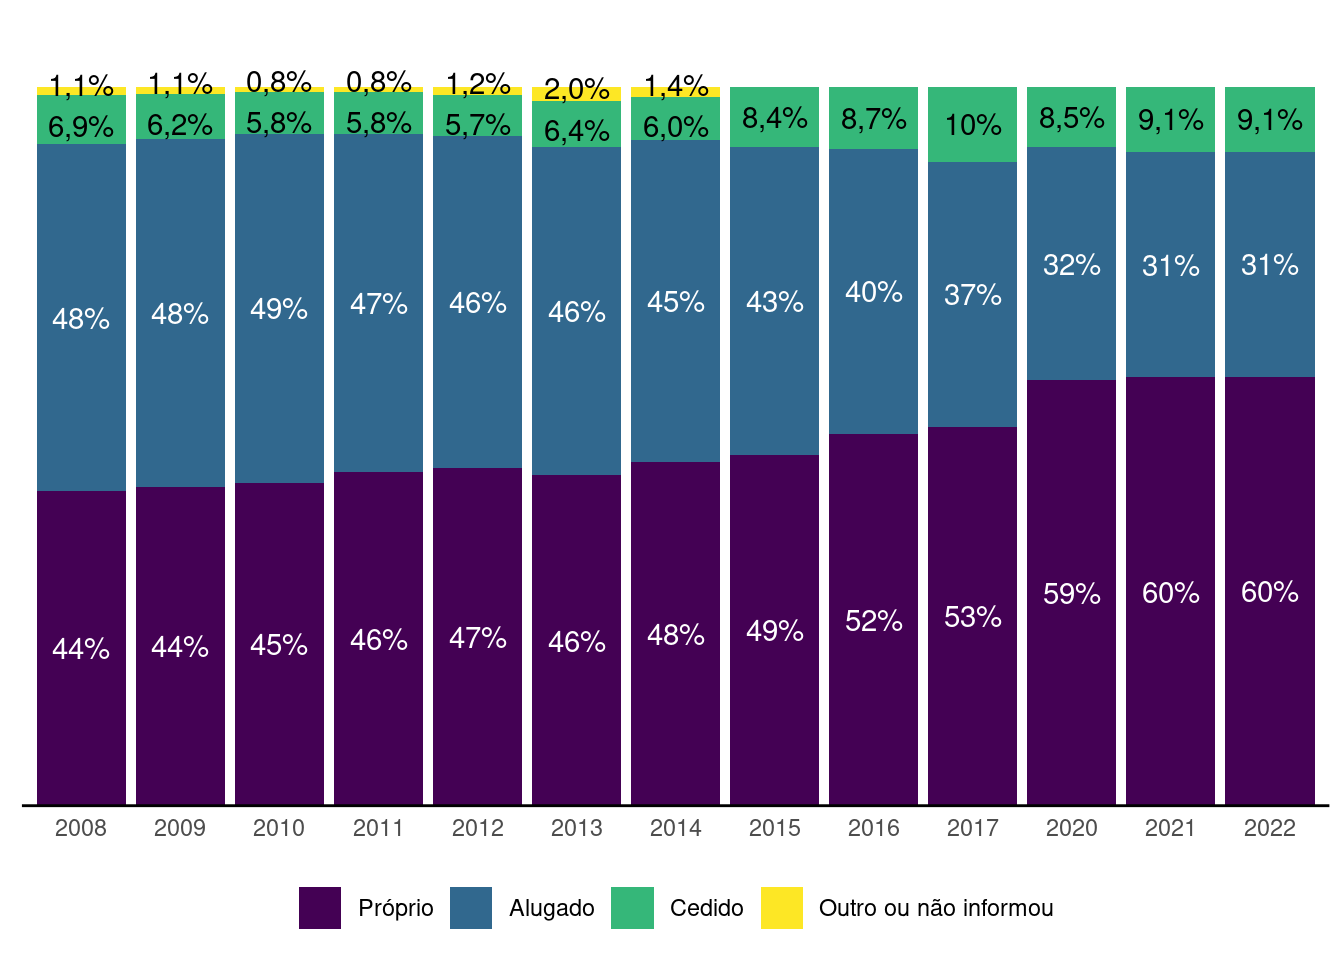
\includegraphics{unidades_files/figure-pdf/fig-CRAS-imovel-1.pdf}

}

\caption{\label{fig-CRAS-imovel}Evolução dos CRAS segundo situação do
imóvel -- Brasil, 2007 a 2022}

\end{figure}%

Ainda sobre o tema da acessibilidade nas unidades de CRAS, observa-se no
Gráfico~\ref{fig-CRAS-acessibilidade} um avanço em todas as condições de
acessibilidade nas unidades de CRAS.\footnote{foram considerados acesso
  adaptado, os imóveis que informam possuir acessibilidade, de acordo
  com a norma ABNT ou não} Apesar da evolução, os dados ainda apontam
para desafios, sobretudo no que se refere a banheiro adaptado que possui
o percentual mais baixo de unidades com essa acessibilidade.

\begin{figure}

\centering{

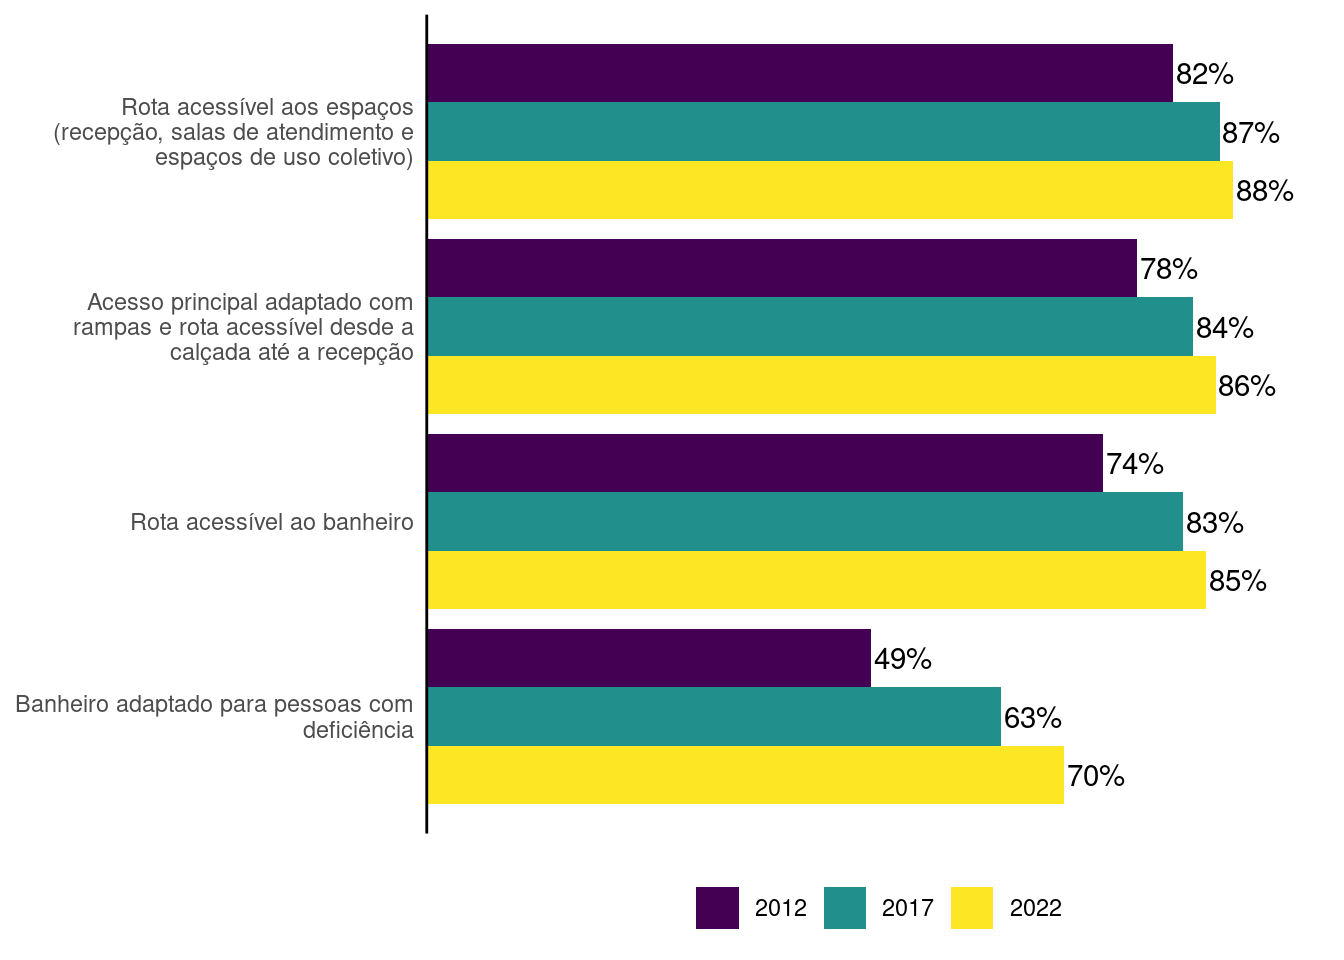
\includegraphics{unidades_files/figure-pdf/fig-CRAS-acessibilidade-1.pdf}

}

\caption{\label{fig-CRAS-acessibilidade}Evolução percentual de CRAS com
condições de acessibilidade - Brasil; 2012, 2017 e 2022}

\end{figure}%

No Gráfico~\ref{fig-CRAS-acessibilidade-situacao} foram relacionadas as
condições de acessibilidade com a situação do imóvel. Em 2022,
verificou-se que as condições de acessibilidade em CRAS localizados em
imóveis próprios possuem números significativamente elevados em relação
aos imóveis alugados ou cedidos.

\begin{figure}

\centering{

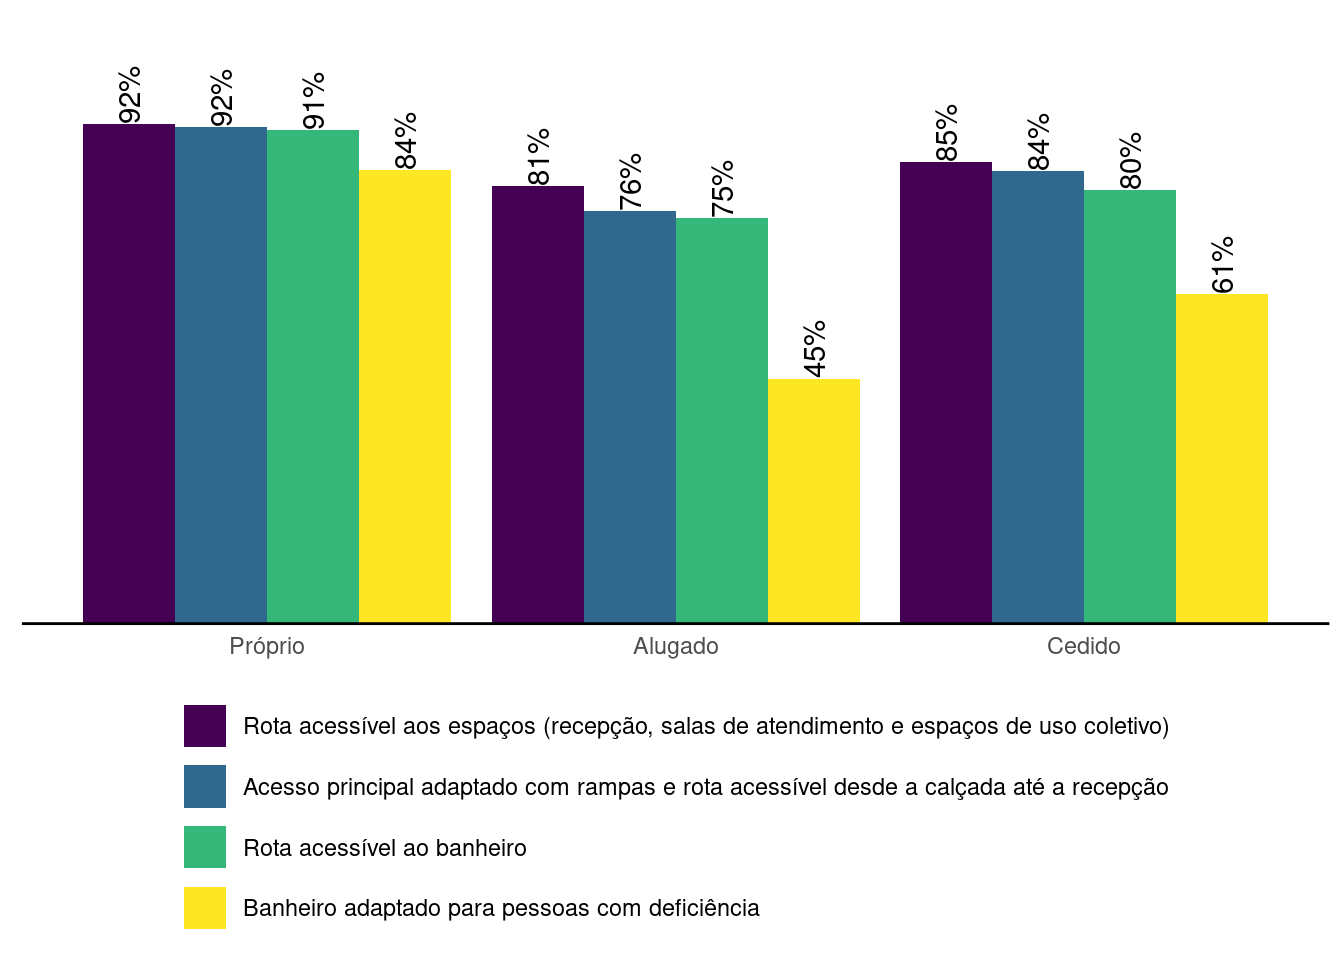
\includegraphics{unidades_files/figure-pdf/fig-CRAS-acessibilidade-situacao-1.pdf}

}

\caption{\label{fig-CRAS-acessibilidade-situacao}Percentual de CRAS com
condições de acessibilidade por situação do imóvel -- Brasil, 2022}

\end{figure}%

Em relação a conectividade, em especial o acesso à internet, o
percentual de CRAS com acesso à internet aumentou significativamente
desde 2007, chegando no último ano desta série com mais de 99\% das
unidades com computadores com acesso à internet, conforme o
Gráfico~\ref{fig-CRAS-internet-percentual}.

\begin{figure}

\centering{

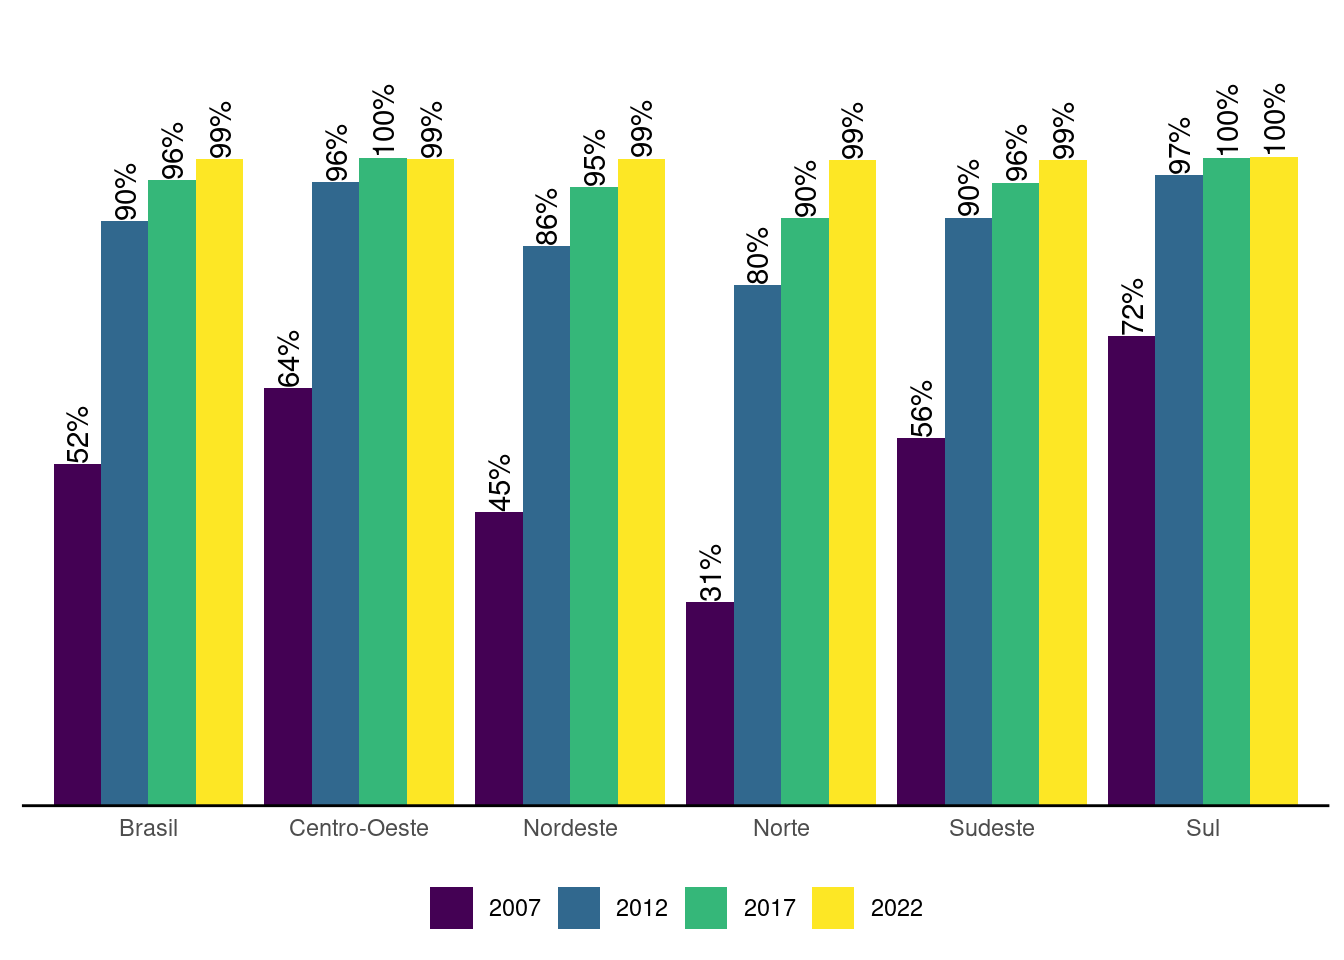
\includegraphics{unidades_files/figure-pdf/fig-CRAS-internet-percentual-1.pdf}

}

\caption{\label{fig-CRAS-internet-percentual}Evolução percentual de CRAS
com computadores com acesso à internet -- Brasil; 2007, 2012, 2017 e
2022}

\end{figure}%

Em relação a CRAS com locais para Cadastro Único, o dado abaixo tráz o
percentual destas informações e a disposição de equipes para esta
finalidade. Nota-se o aumento ao longo dos anos, das unidades de CRAS
que possuem Cadastro Único com equipe exclusiva, chegando no Censo SUAS
de 2022 com 59\% (Gráfico~\ref{fig-equip-cadunico-cras}).

\begin{figure}

\centering{

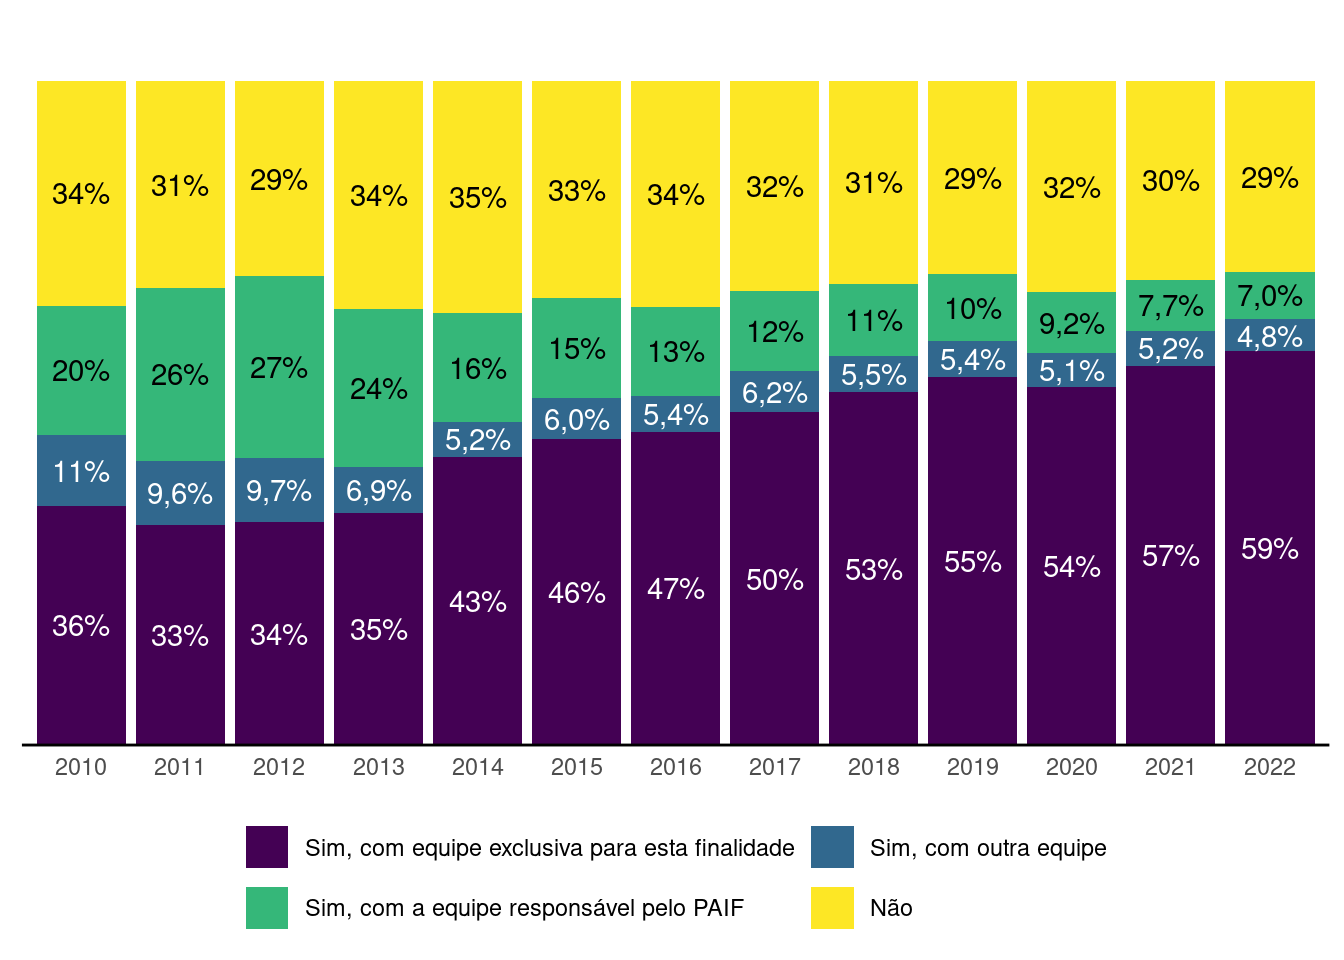
\includegraphics{unidades_files/figure-pdf/fig-equip-cadunico-cras-1.pdf}

}

\caption{\label{fig-equip-cadunico-cras}Percentual de CRAS com locais
para CadÚnico - 2017 - 2022}

\end{figure}%

\section{Centros de Convivência}\label{centros-de-convivuxeancia}

Os Centros de Convivência, são unidades que executam o Serviço de
Convivência e Fortalecimento de Vínculos (SCFV) e compõem a Rede de
Proteção Social Básica. Desde 2014 o número de Centros de Convivência no
Brasil vem aumentando, passando de 7.882 unidades em 2014 para 8.454 em
2016, acréscimo de 572 unidades. A região Norte tem a menor quantidade
de unidades (238 ou 2,8\% do total), seguida do Centro-Oeste com 568
Unidades (ou 6,7\% do total). A região Sudeste tem o maior número de
Centros de Convivência, com 4.035 Unidades (47,7\% do total).

Os Centros de Convivência podem ser unidades públicas ou vinculadas a
entidades de assistência social inscritas nos Conselhos de Assistência
Social do município ou do Distrito Federal. Em 2022, 44\% dos Centros de
Convivência eram governamentais e 56\% das unidades eram não
governamentais. \footnote{os dados de 2016 não foi possível de ser
  coletato devido a dificuldades de leitura da base de dados}

\begin{figure}

\centering{

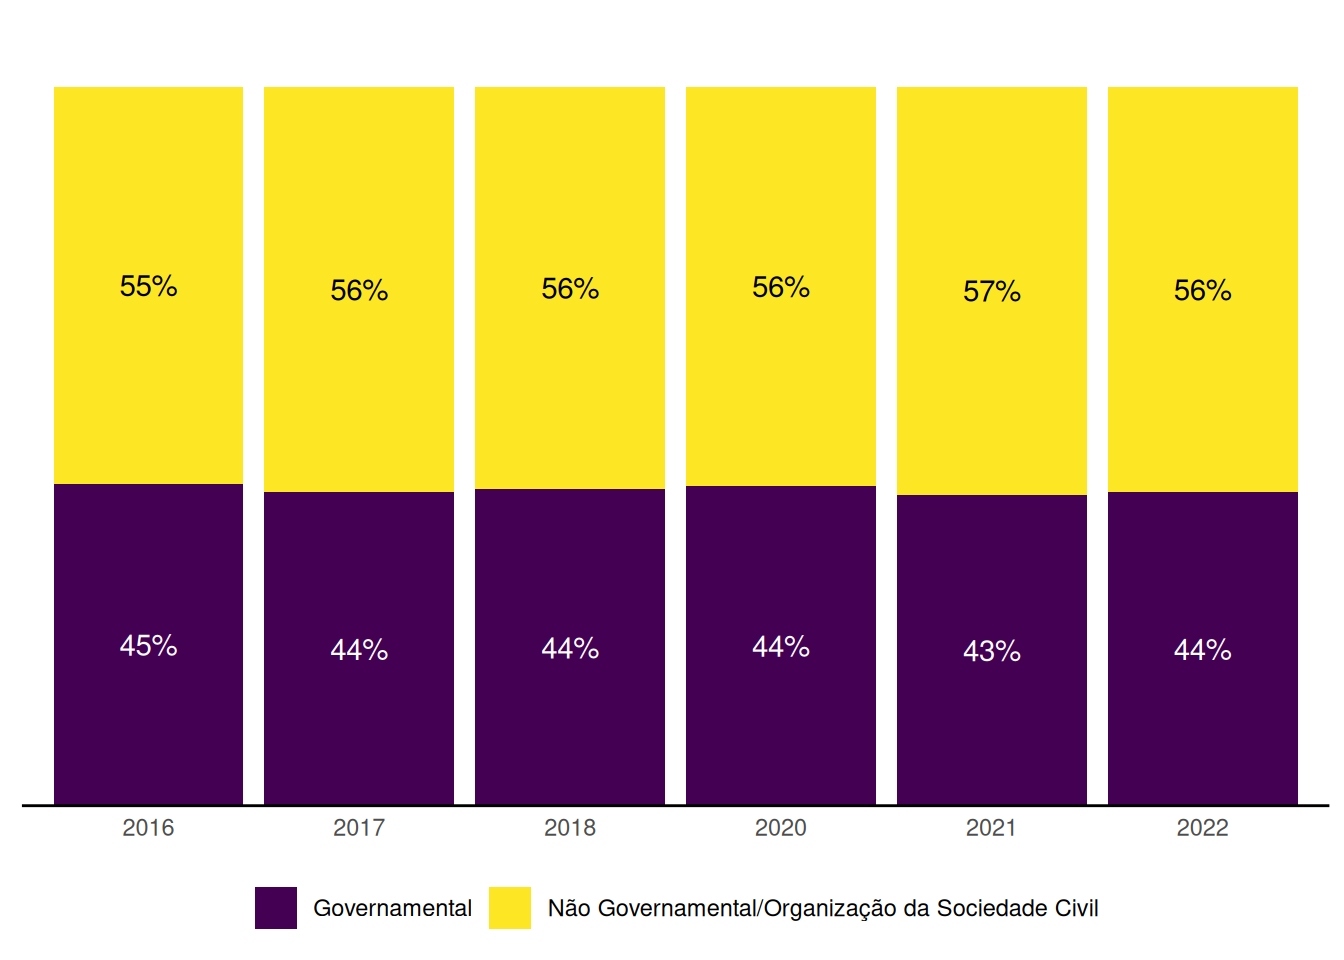
\includegraphics{unidades_files/figure-pdf/fig-centro-conv-natureza-1.pdf}

}

\caption{\label{fig-centro-conv-natureza}Quantitativo de Centros de
Convivência por Natureza da Unidade - BRASIL; 2016 a 2022}

\end{figure}%

\section{Centro de Referência Especializada de Assistência Social
(CREAS)}\label{centro-de-referuxeancia-especializada-de-assistuxeancia-social-creas}

Os Centros de Referência Especializados de Assistência Social (CREAS)
são unidades públicas estatais que ofertam serviços da proteção social
especial a pessoas e famílias em situação de risco pessoal ou social
e/ou em situação de violação de direitos.

O Censo SUAS 2022 registrou 2.846 CREAS no país: um incremento de 679
novas unidades em relação aos últimos 10 anos. O
Gráfico~\ref{fig-creas-quantitativo} sinaliza esta evolução por Regiões
do país.

\begin{figure}

\centering{

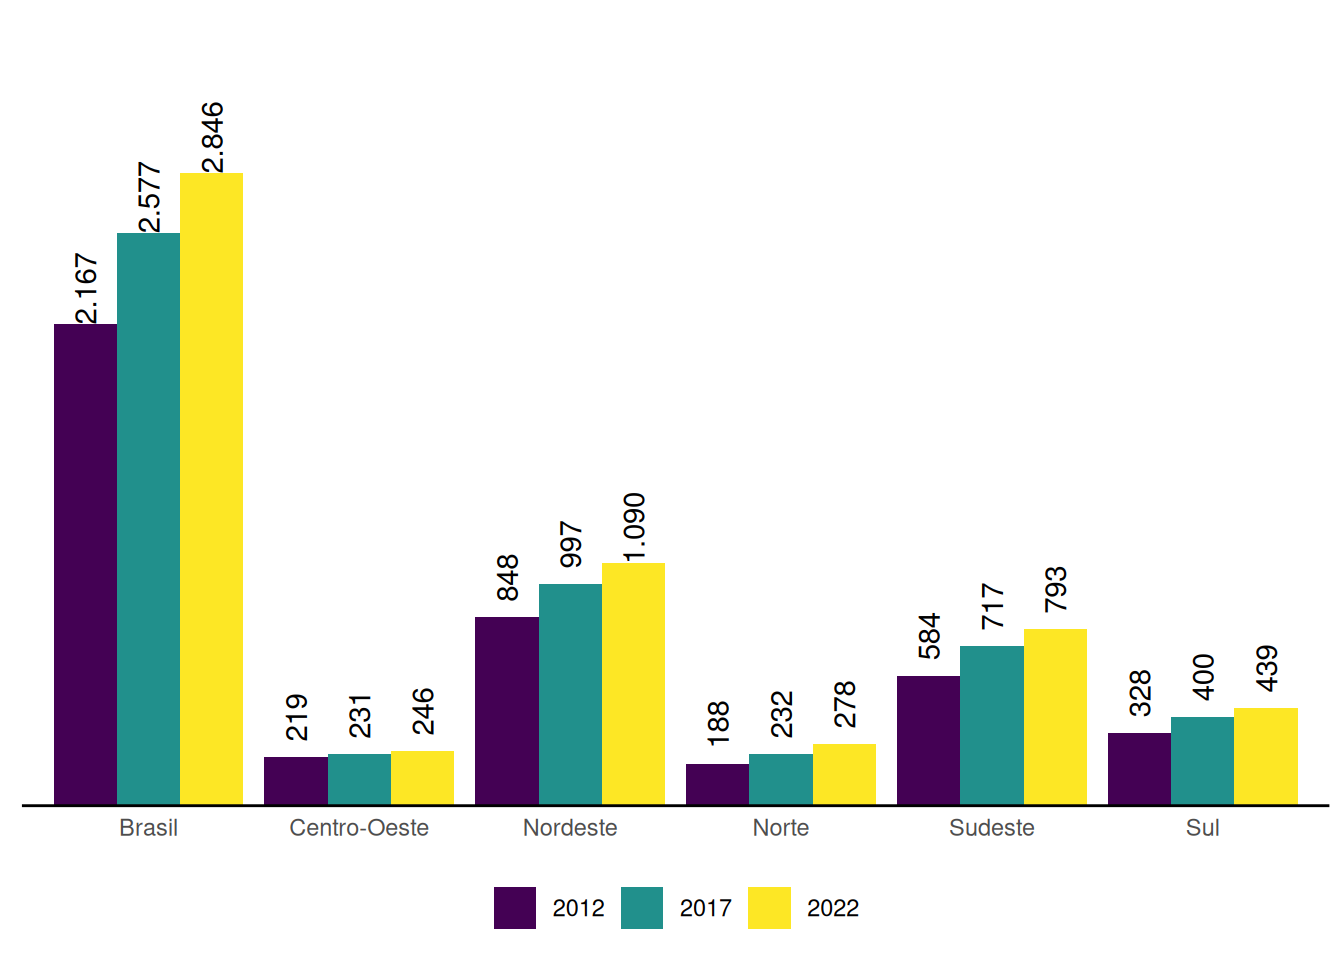
\includegraphics{unidades_files/figure-pdf/fig-creas-quantitativo-1.pdf}

}

\caption{\label{fig-creas-quantitativo}Evolução do quantitativo de
CREAS, segundo grandes regiões; 2012, 2017 e 2022}

\end{figure}%

De acordo com os dados do Gráfico~\ref{fig-CREAS-porte}, que mostra o
número de CREAS por município levando-se em conta o porte populacional,
verifica-se que 54\% dos municípios não possuem CREAS. Eles estão
concentrados nos municípios de Pequeno Porte I e II, com respectivamente
77\% e 5,3\% dos municípios que não possuem esta unidade especializada.

\begin{figure}

\centering{

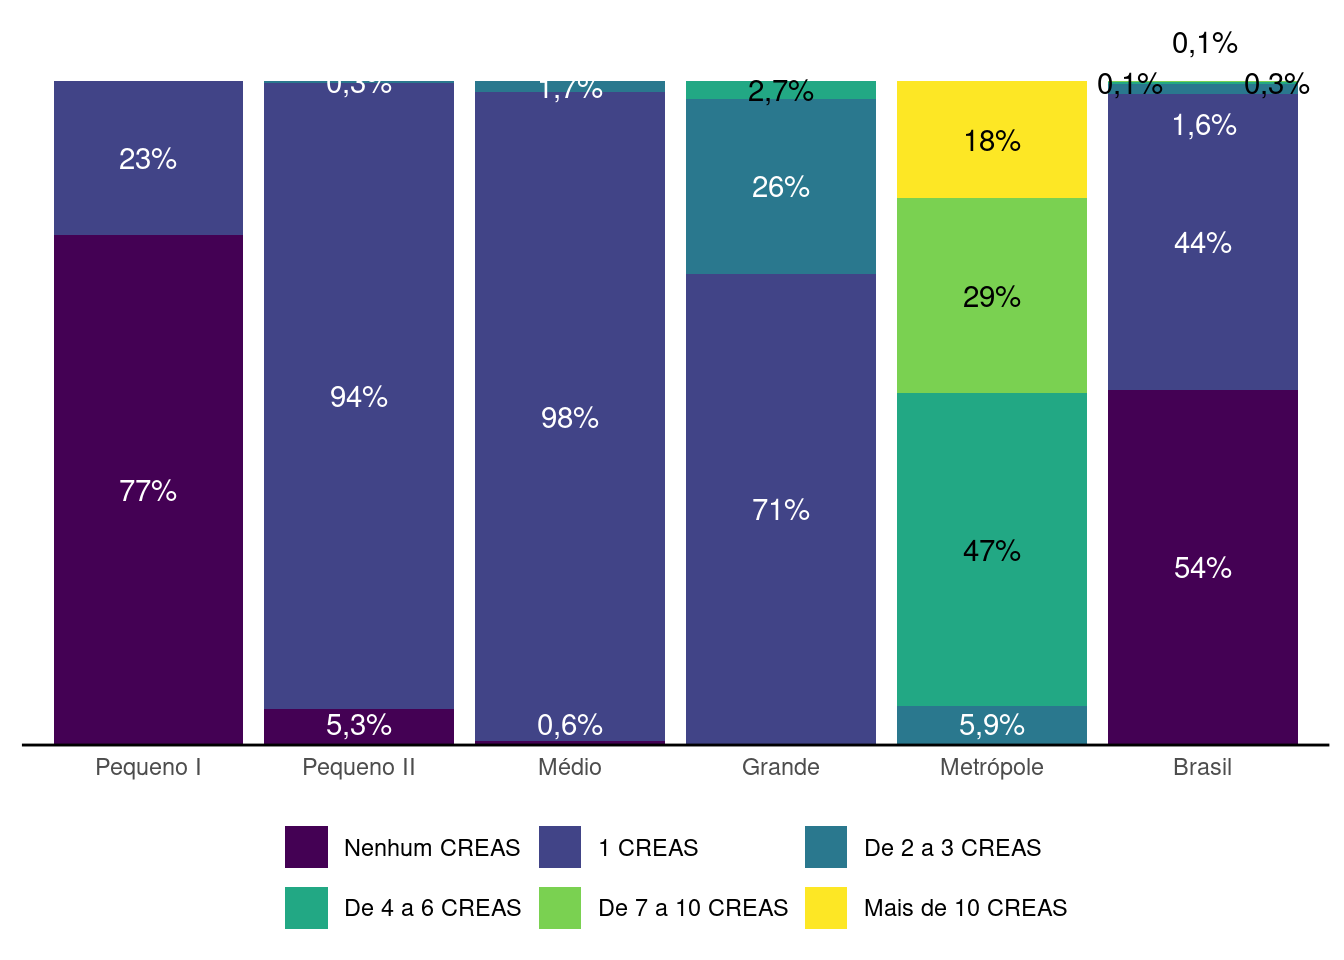
\includegraphics{unidades_files/figure-pdf/fig-CREAS-porte-1.pdf}

}

\caption{\label{fig-CREAS-porte}Percentual de municípios por número de
CREAS, segundo porte populacional - Brasil, 2022}

\end{figure}%

Ao observar a série histórica do Gráfico~\ref{fig-creas-situacao} é
possível perceber que os imóveis próprios vem aumentando ao longo do
tempo. Em 2012 eram 27\% das unidades e, em 2022 37\% destas unidades
passam a possuir imóveis prórpios. Ao passo que os imóveis próprios
aumentam em 10\% pontos percentuais, os imovéis alugados decrescem,
computado no Censo SUAS de 2022 com 57\% das unidades alugadas.Há também
registros de imóveis cedidos no qual ao longo dos anos sinalizam um leve
aumento\footnote{Para os anos de 2018 e 2019 esse dado não foi computado
  no Censo SUAS}.

\begin{figure}

\centering{

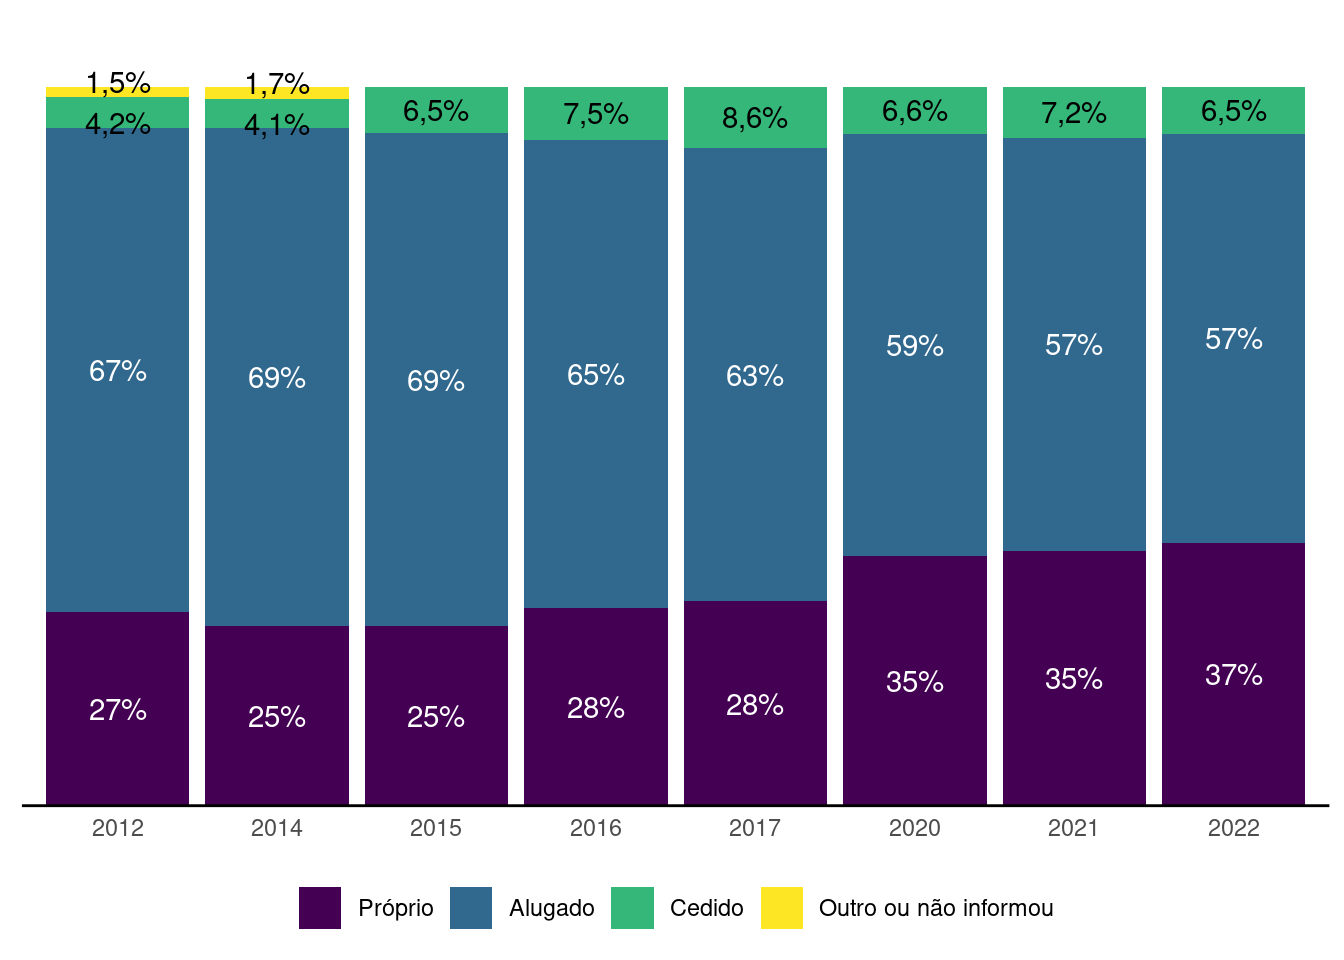
\includegraphics{unidades_files/figure-pdf/fig-creas-situacao-1.pdf}

}

\caption{\label{fig-creas-situacao}Evolução dos CREAS segundo situação
do imóvel -- Brasil; 2012 a 2022}

\end{figure}%

De acordo com os dados do Censo SUAS do período de 2012 a 2022, houve
aumento das condições de acessibilidade em vários itens dos CREAS. O
Gráfico~\ref{fig-creas-acessibilidade} sinaliza que a presença do acesso
principal adaptado com rota ascessível aos espaços (recepção, salas de
atendimento e espaços de uso coletivo) é a mais presente nas unidades de
CREAS, com destaque para 83\% no CENSO SUAS de 2022.

O dado proporcional menos presente nas unidades de CREAS é o Banheiro
adaptado. Em de 2012, 33\% dos CREAS foram identificados com banheiro
adaptado. Esse mesmo dado em 2022 chegou a 55\% dos CREAS. Destaca-se um
crescimento de 22 pontos percentuais em relação ao ano de 2012.
\footnote{foram considerados acesso adptado os imóveis que informam
  possuir acessibilidade, de acordo com a norma ABNT ou não}.

\begin{figure}

\centering{

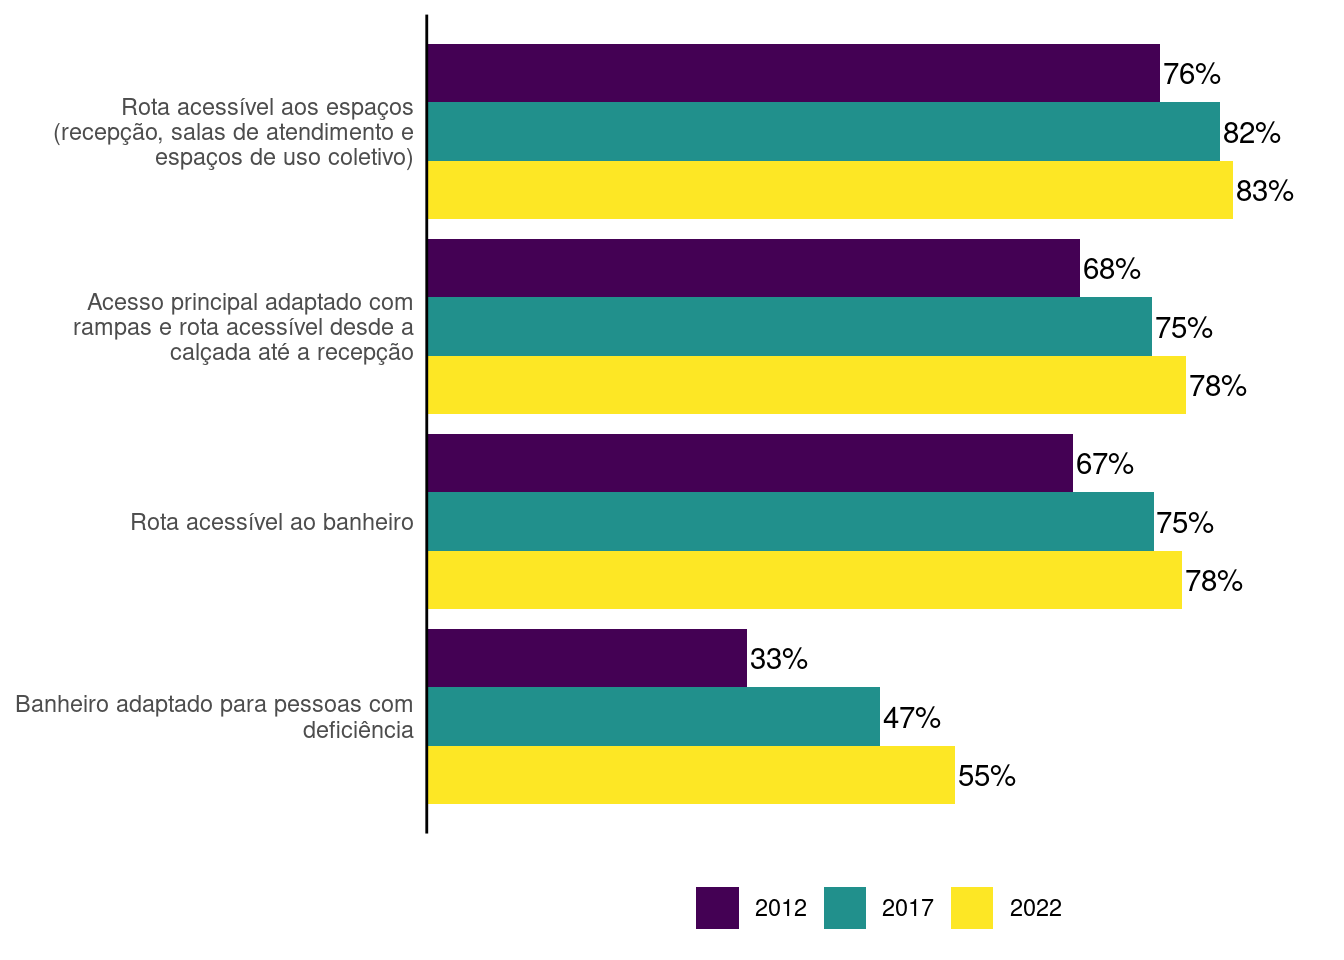
\includegraphics{unidades_files/figure-pdf/fig-creas-acessibilidade-1.pdf}

}

\caption{\label{fig-creas-acessibilidade}Evolução percentual de CREAS
com condições de acessibilidade - Brasil; 2012, 2017 e 2022}

\end{figure}%

O Gráfico~\ref{fig-CREAS-acessibilidade-situacao} mostra a presença de
condições de acessibilidade segundo a situação do imóvel. Os dados
sinalizam que a acessibilidade é significativamente mais presente em
imovéis próprios.

\begin{figure}

\centering{

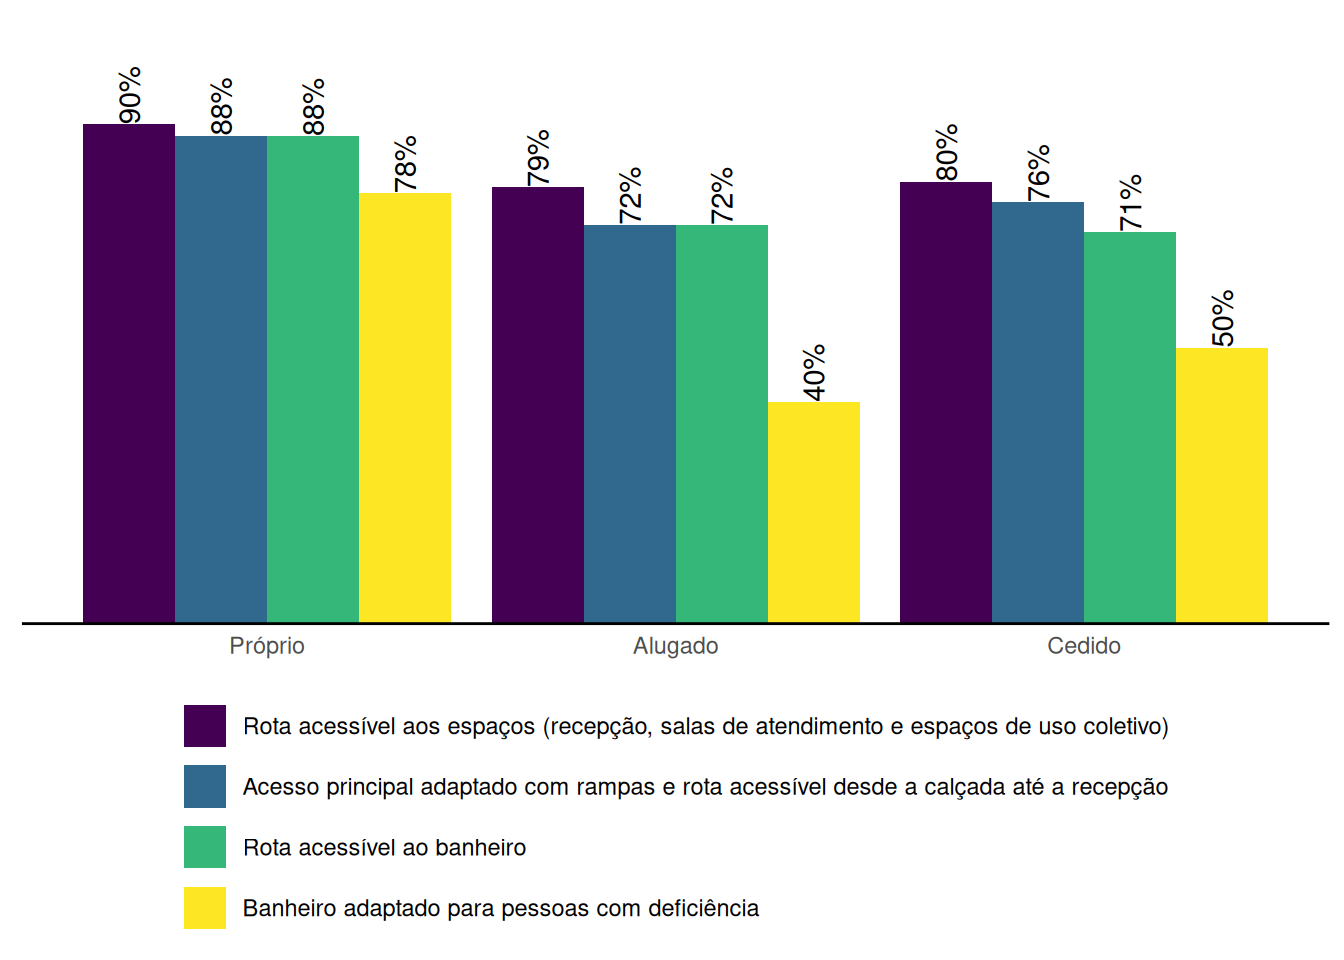
\includegraphics{unidades_files/figure-pdf/fig-CREAS-acessibilidade-situacao-1.pdf}

}

\caption{\label{fig-CREAS-acessibilidade-situacao}Evolução percentual de
CREAS com condições de acessibilidade por situação do imóvel -- Brasil,
2022}

\end{figure}%

A existência de computadores com acesso à internet é um importante
aspecto a ser observado quando se avalia a infraestrutura dos CREAS. No
período de 2012 a 2022, observa-se que este item avançou de 89\% para
99\% dos CREAS que possuem computadores com acesso à internet conforme o
Gráfico~\ref{fig-CREAS-internet-percentual}.

Esses números avançaram em todas as regiões, em especial, na Região
Norte conforme pode ser observado no
Gráfico~\ref{fig-CREAS-internet-percentual}.

\begin{figure}

\centering{

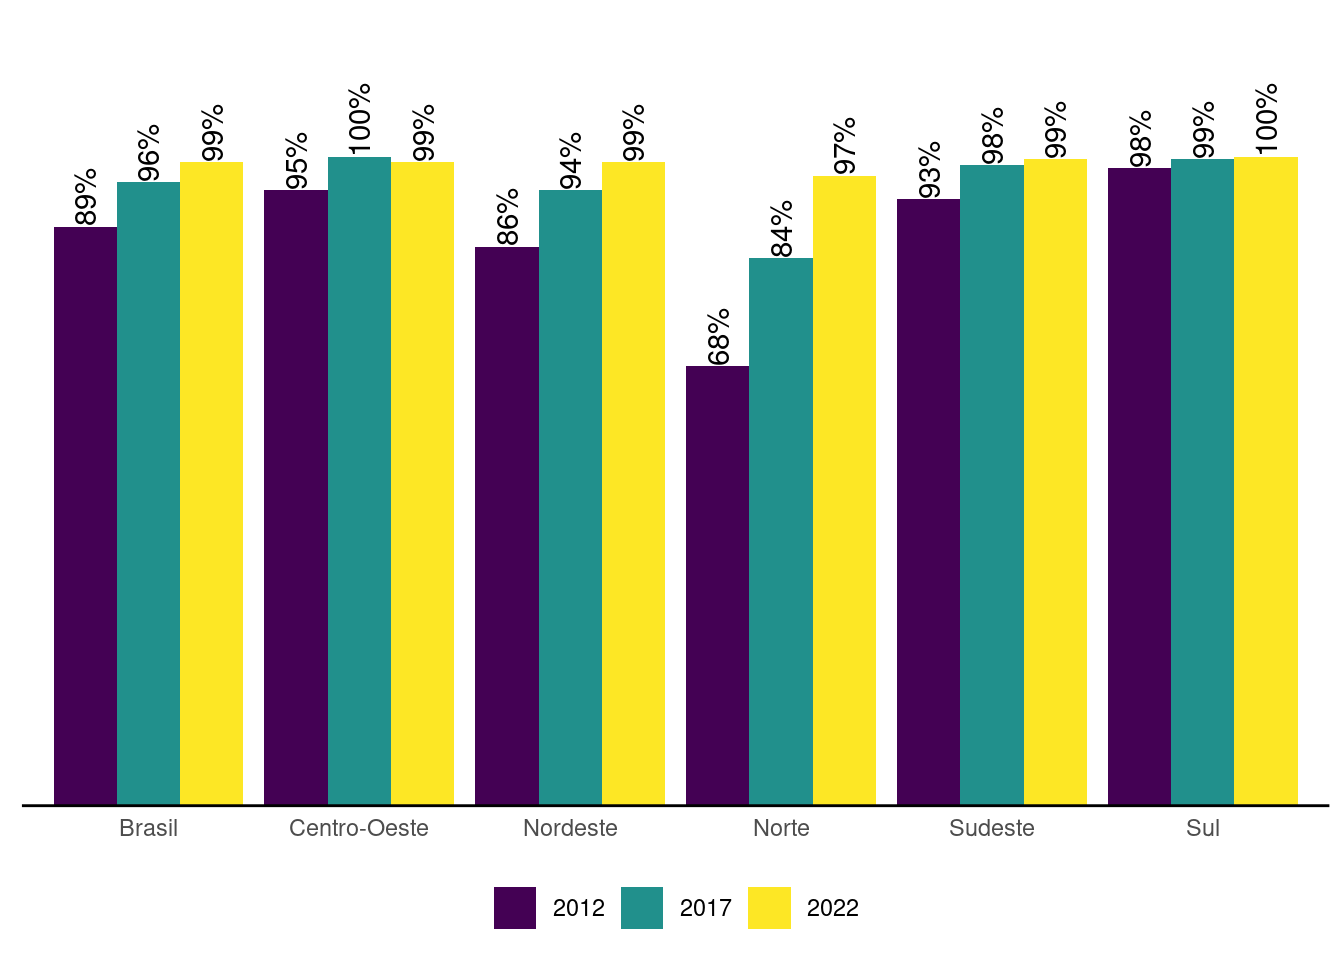
\includegraphics{unidades_files/figure-pdf/fig-CREAS-internet-percentual-1.pdf}

}

\caption{\label{fig-CREAS-internet-percentual}Evolução percentual de
CREAS com computadores com acesso à internet -- Brasil, 2012 - 2022}

\end{figure}%

A oferta regionalizada de CREAS é uma estratégia que objetiva garantir a
universalização do acesso e integralidade do antendimento da proteção
socioassistencia especializada. Ela está prevista através da Resolução
CNAS 31/2013. Essa composição é organizada através dos entes estaduais.
O Gráfico~\ref{fig-creas-regionais} sinaliza a evolução dessa oferta.

\begin{figure}

\centering{

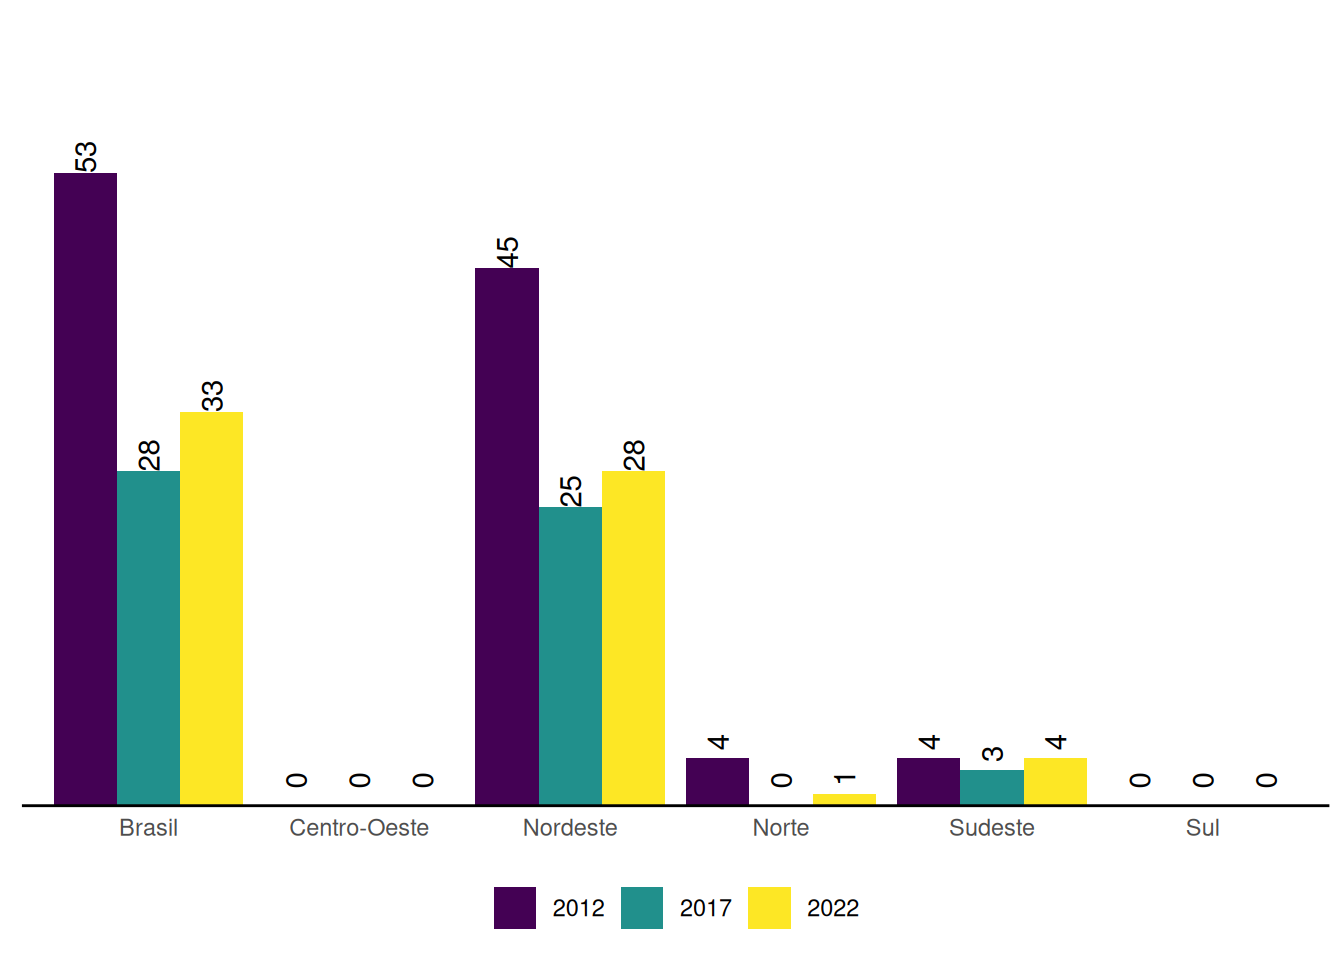
\includegraphics{unidades_files/figure-pdf/fig-creas-regionais-1.pdf}

}

\caption{\label{fig-creas-regionais}Evolução do quantitativo de CREAS
Regionais, Brasil e grandes regiões - 2012, 2017 e 2022}

\end{figure}%

\section{Centro de Referência Especializado para População em Situação
de Rua (Centro
POP)}\label{centro-de-referuxeancia-especializado-para-populauxe7uxe3o-em-situauxe7uxe3o-de-rua-centro-pop}

Os Centros de Referência Especializados para População em Situação de
Rua (Centros POP) são unidades públicas que oferecem atendimento
especializado para a população em situação de rua, no âmbito da proteção
social especial de média complexidade.

Entre 2012 e 2022 o número de Centros POP cresceu, passando de 105
unidades para 237 no período. O Gráfico~\ref{fig-quantitativo-CentroPop}
sinaliza essa evolução na escala de a cada 5 anos por Regiões do Brasil.

\begin{figure}

\centering{

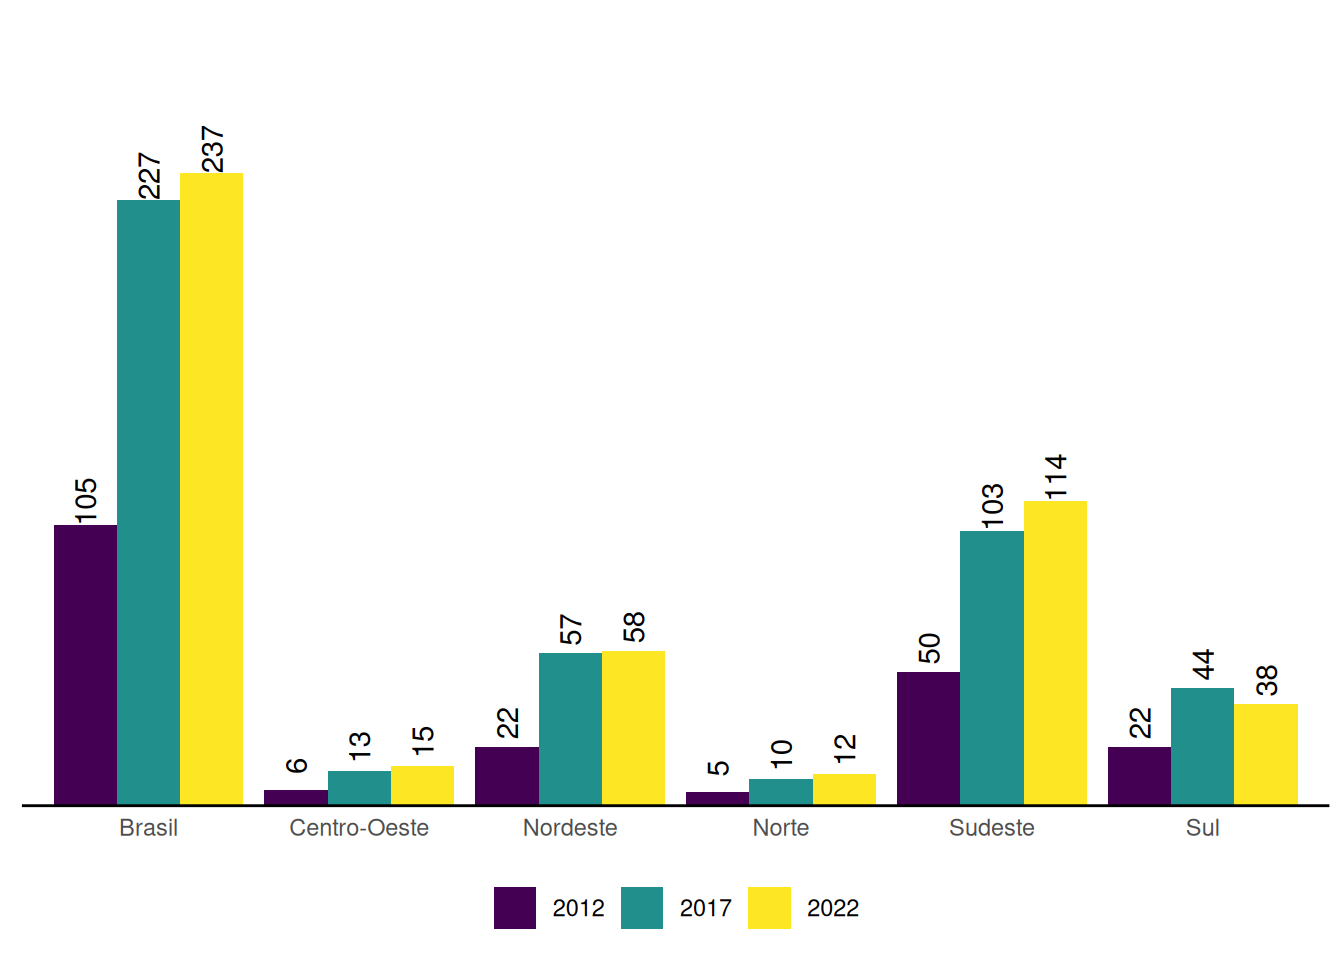
\includegraphics{unidades_files/figure-pdf/fig-quantitativo-CentroPop-1.pdf}

}

\caption{\label{fig-quantitativo-CentroPop}Evolução do quantitativo de
Centro POP, 2012 a 2022}

\end{figure}%

Os Centros Pop estão presentes em municípios de grande porte e
metrópole, o Gráfico~\ref{fig-cpop-porte} sinaliza que 59\% dos
municípios de grande porte possuem pelo menos uma unidade. Nas
metrópoles, 100\% possuem unidades de Centro POP, sendo 59\% entre duas
a três unidades, 24\% uma unidade e 18\% de 4 a 6 unidades. Esta unidade
também está presente em municípios de médio porte, com destaque para
5,9\% dos municípios.

\begin{figure}

\centering{

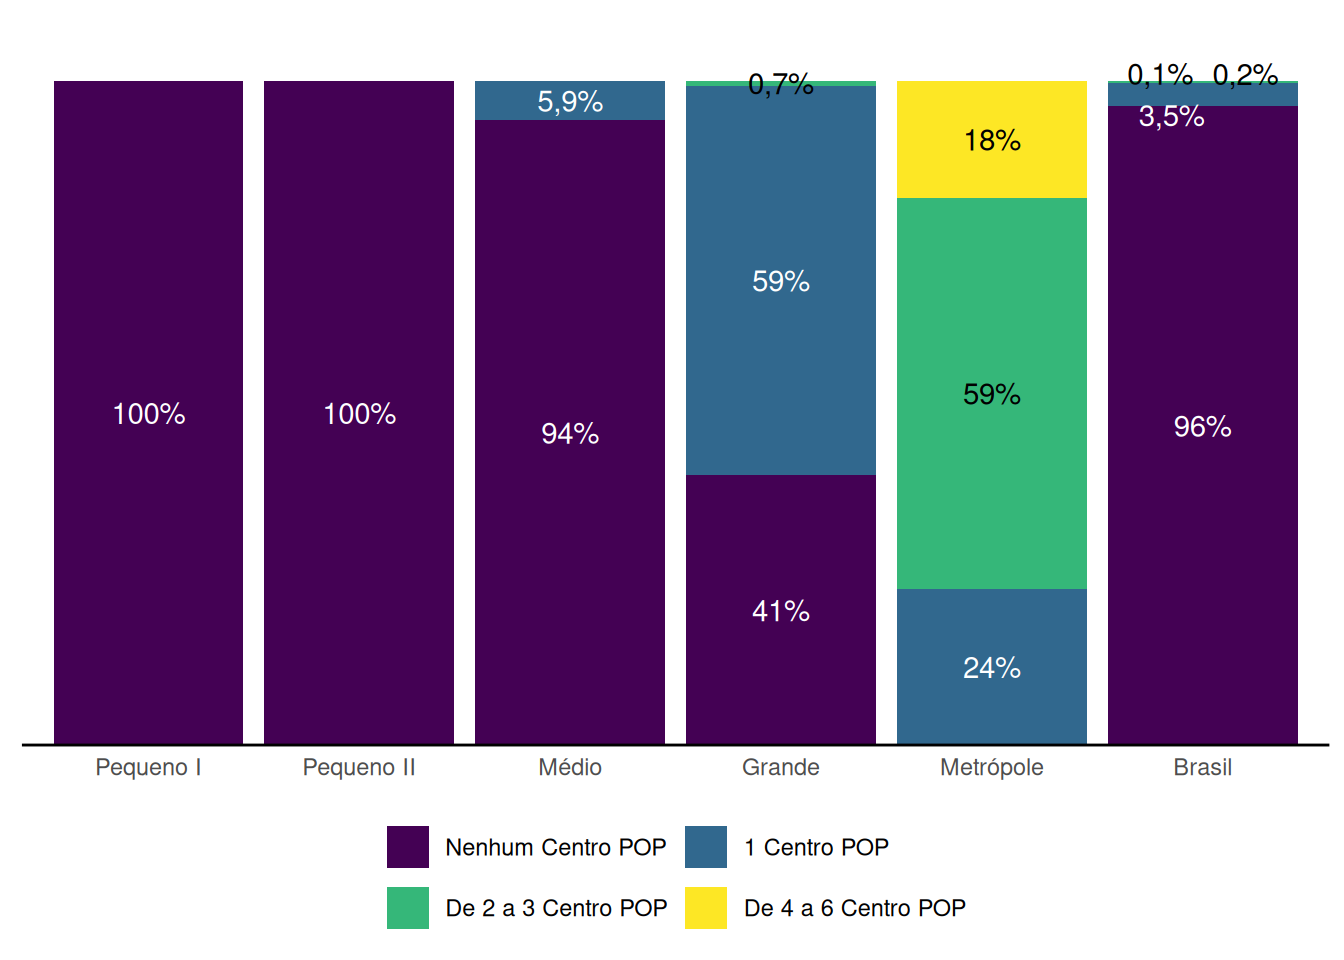
\includegraphics{unidades_files/figure-pdf/fig-cpop-porte-1.pdf}

}

\caption{\label{fig-cpop-porte}Percentual de municípios por número de
Centro POP, segundo porte populacional - Brasil, 2022}

\end{figure}%

Em relação a acessibilidade dos Centro POP, o
Gráfico~\ref{fig-cpop-acessibilidade-situacao} relaciona esta adaptação
com a situação do imóvel. No geral todas as adaptações de acessibilidade
são superiores ao serem relacionadas com os imóveis alugados. Em relação
aos imóveis cedidos, a adaptação de banheiro se sobressai em relação as
demais situações dos imóveis.

\begin{figure}

\centering{

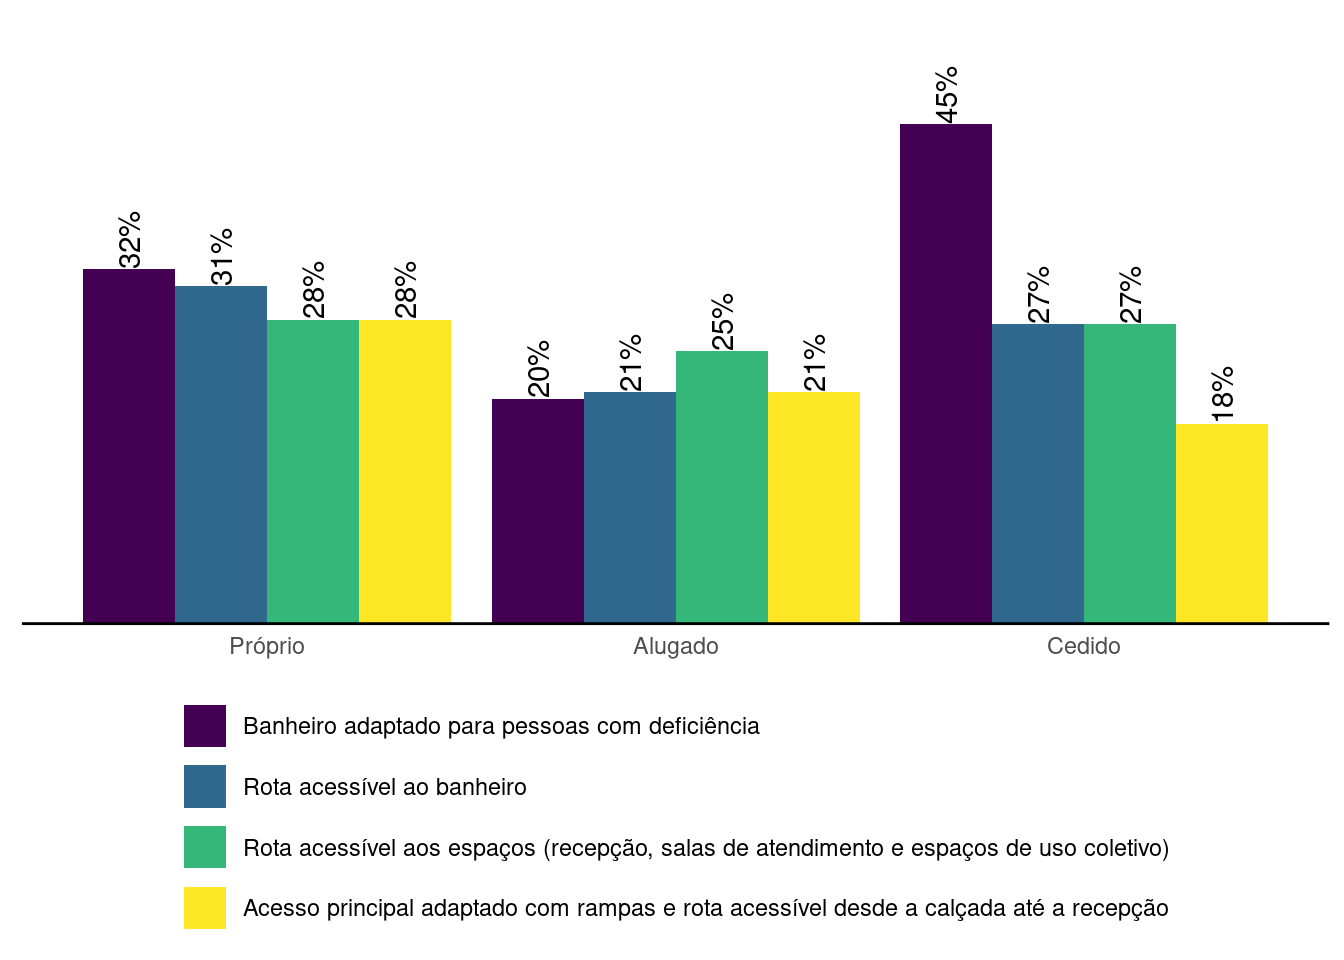
\includegraphics{unidades_files/figure-pdf/fig-cpop-acessibilidade-situacao-1.pdf}

}

\caption{\label{fig-cpop-acessibilidade-situacao}Percentual de Centros
POP com condições de acessibilidade segundo situação do imóvel --
Brasil, 2022}

\end{figure}%

Em 2016,95\% dos Centros Pop destacam computador com acesso à internet
em 2022. O Gráfico~\ref{fig-cpop-internet-percentual} referencia essa
evolução por Regiões do Brasil, as regiões Centro Oeste e Sul possuem
100\% das unidades com acesso à internet e a região Norte com maior
desafio de acesso, com 75\% das unidades de Centro POP com acesso à
internet.

\begin{figure}

\centering{

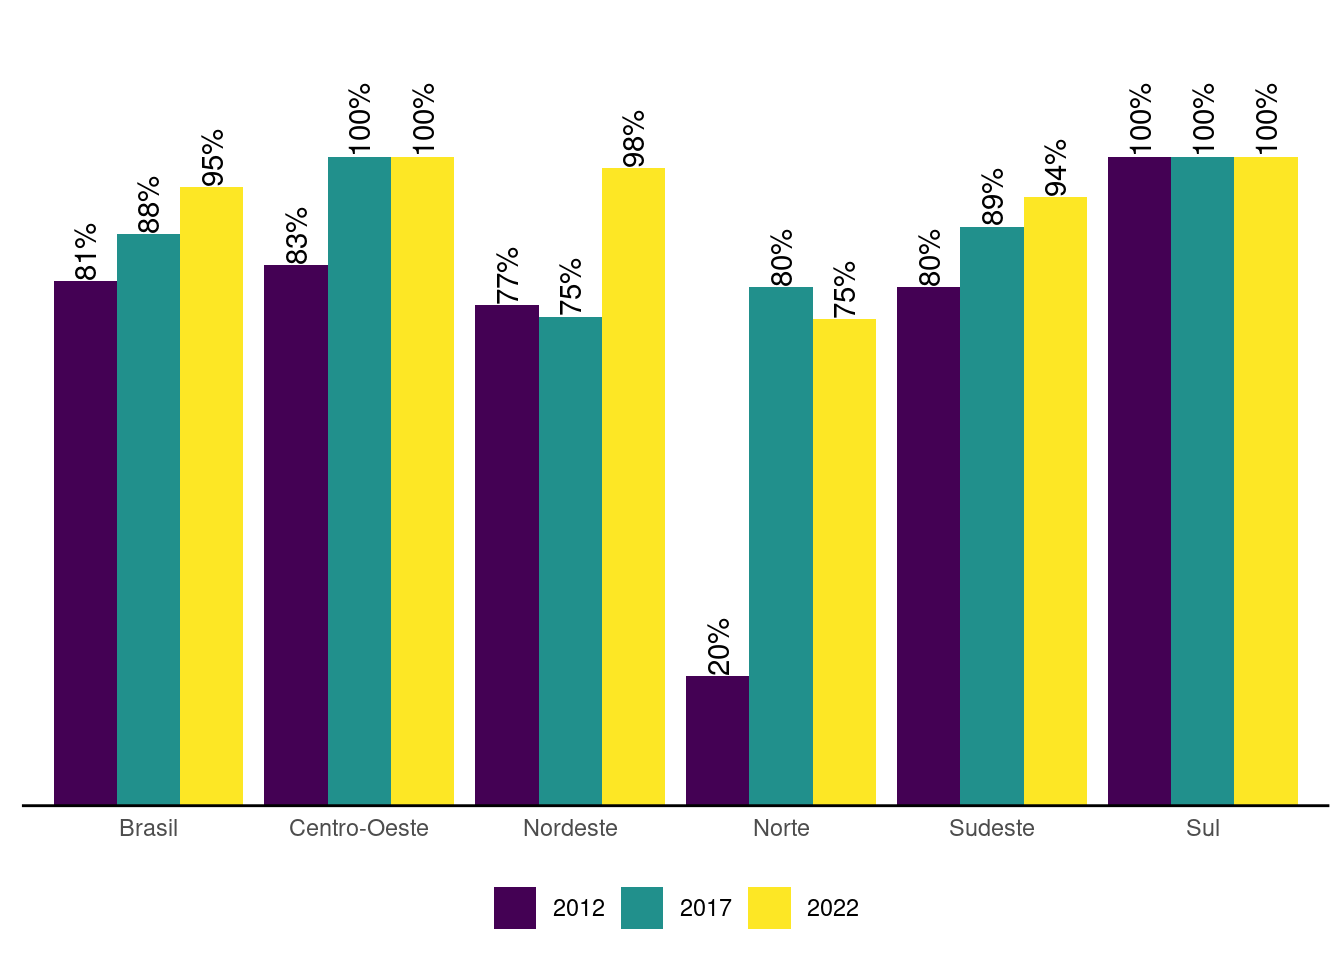
\includegraphics{unidades_files/figure-pdf/fig-cpop-internet-percentual-1.pdf}

}

\caption{\label{fig-cpop-internet-percentual}Percentual de Computadores
nos Centro POP com acesso à internet, 2012 a 2022}

\end{figure}%

\section{Centro-Dia}\label{centro-dia}

Os Centros Dia são unidades públicas especializadas para atender pessoas
com deficiência e suas famílias. Ela está inserida no âmbito da proteção
social especial de média complexidade. No ano de 2015 identifica-se no
Brasil 1.340 unidades. Em 2022 há um crescimento de 40,7\% destas
unidades, conforme pode ser observada no
Gráfico~\ref{fig-quantitativo-Centrodia}.

\begin{figure}

\centering{

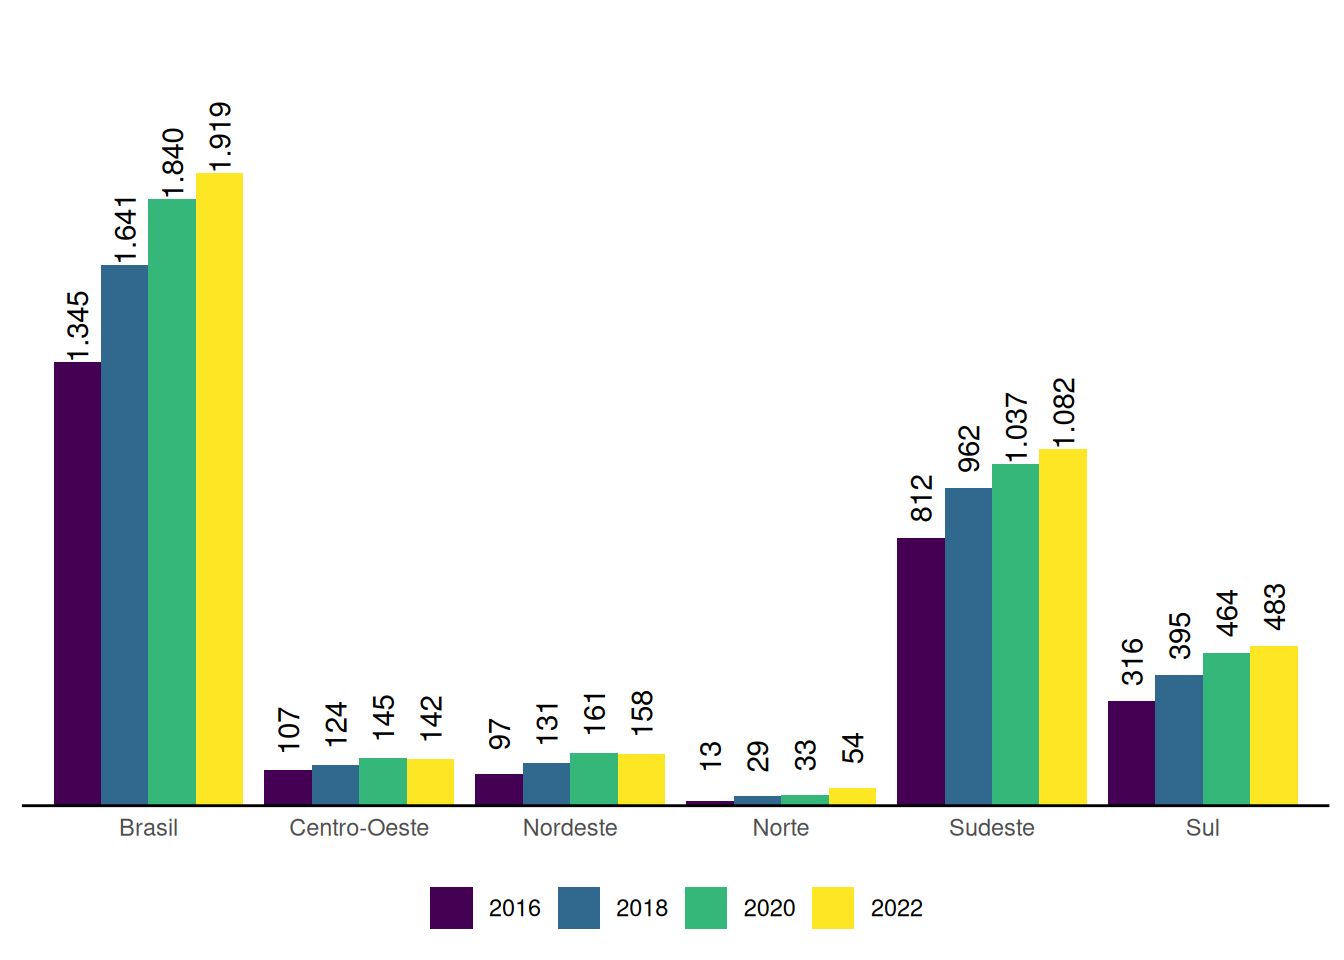
\includegraphics{unidades_files/figure-pdf/fig-quantitativo-Centrodia-1.pdf}

}

\caption{\label{fig-quantitativo-Centrodia}Evolução do quantitativo de
Centro-Dia, segundo grandes regiões; 2016 a 2022}

\end{figure}%

Em relação a natureza destas unidades, o Gráfico~\ref{fig-cdia-natureza}
sinaliza que estas unidades são majoritariamente referenciadas pelas
Organizações da Sociedade Civil (OSCs). Das unidades destacadas no Censo
SUAS 2022, 92,8\% são ofertadas por OSCs.\footnote{não foi identificado
  essa pergunta para o ano de 2017 e para o ano de 2022 não foi possível
  gerar a informação a partir do banco de dados disponível}

\begin{figure}

\centering{

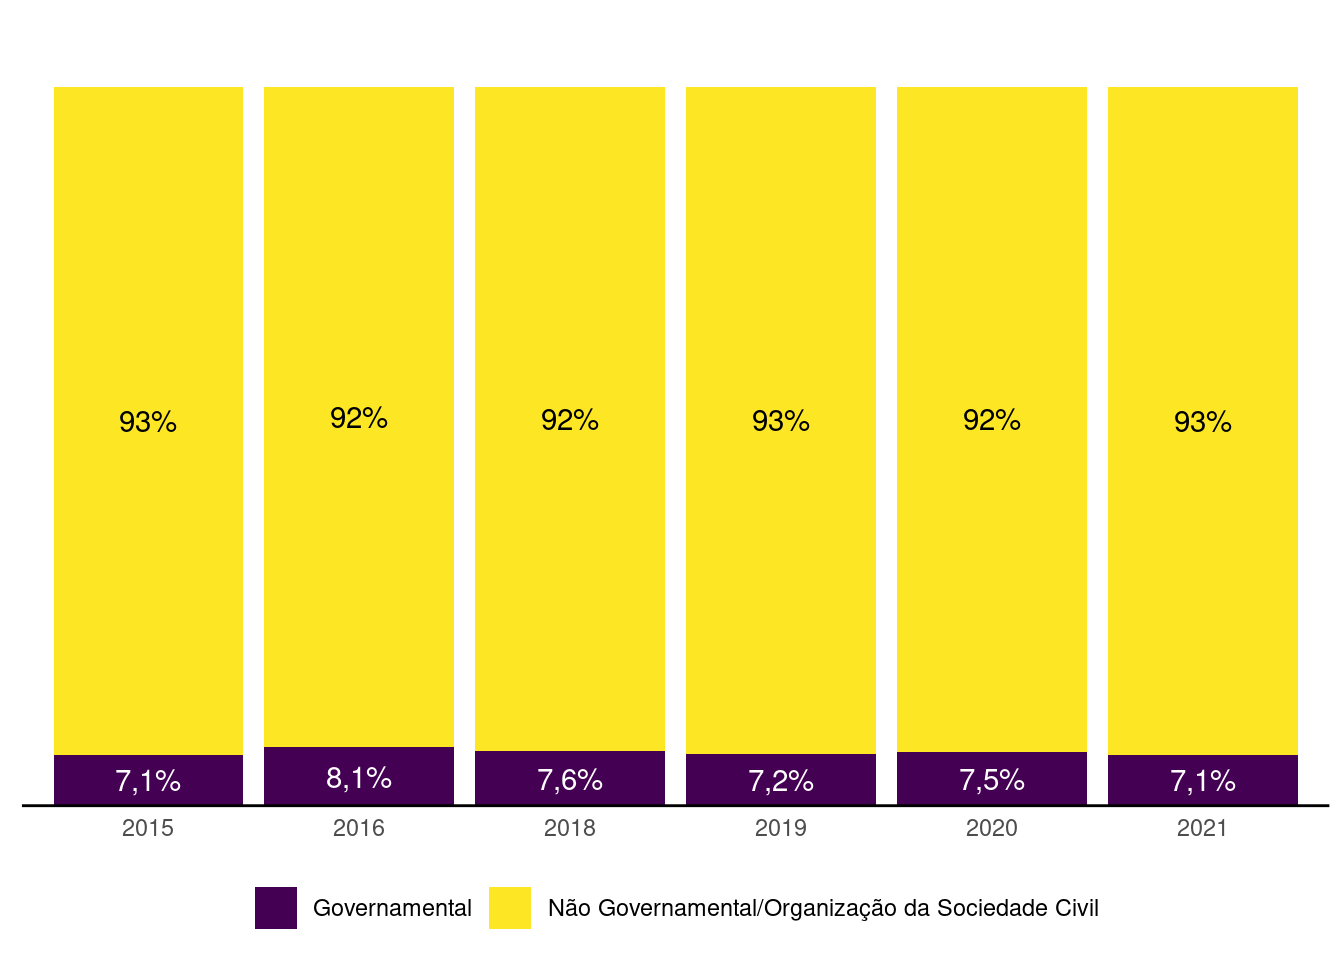
\includegraphics{unidades_files/figure-pdf/fig-cdia-natureza-1.pdf}

}

\caption{\label{fig-cdia-natureza}Quantitativo de Centros Dia por
Natureza da Unidade - BRASIL, 2015 a 2022}

\end{figure}%

Em relação a acessibilidade destas unidades, o banheiro acessivel é a
adaptação mais presentes nestas unidades chegando nos registros do Censo
SUAS de 2022 com 73\%. Como trata-se de unidades especializadas para
atenção a pessoas com deficiência, esse item é de fundamental
importância para assegurar acolhida e segurança a este público e suas
famílias. O Gráfico~\ref{fig-cdia-acessibilidade} sinaliza os locais e
composição de acessibilidade, estes dados sinalizam um desafio para
garantir as condições físicas de acesso ao público de pessoas com
deficiência nas unidades de Centro-Dia.

\begin{figure}

\centering{

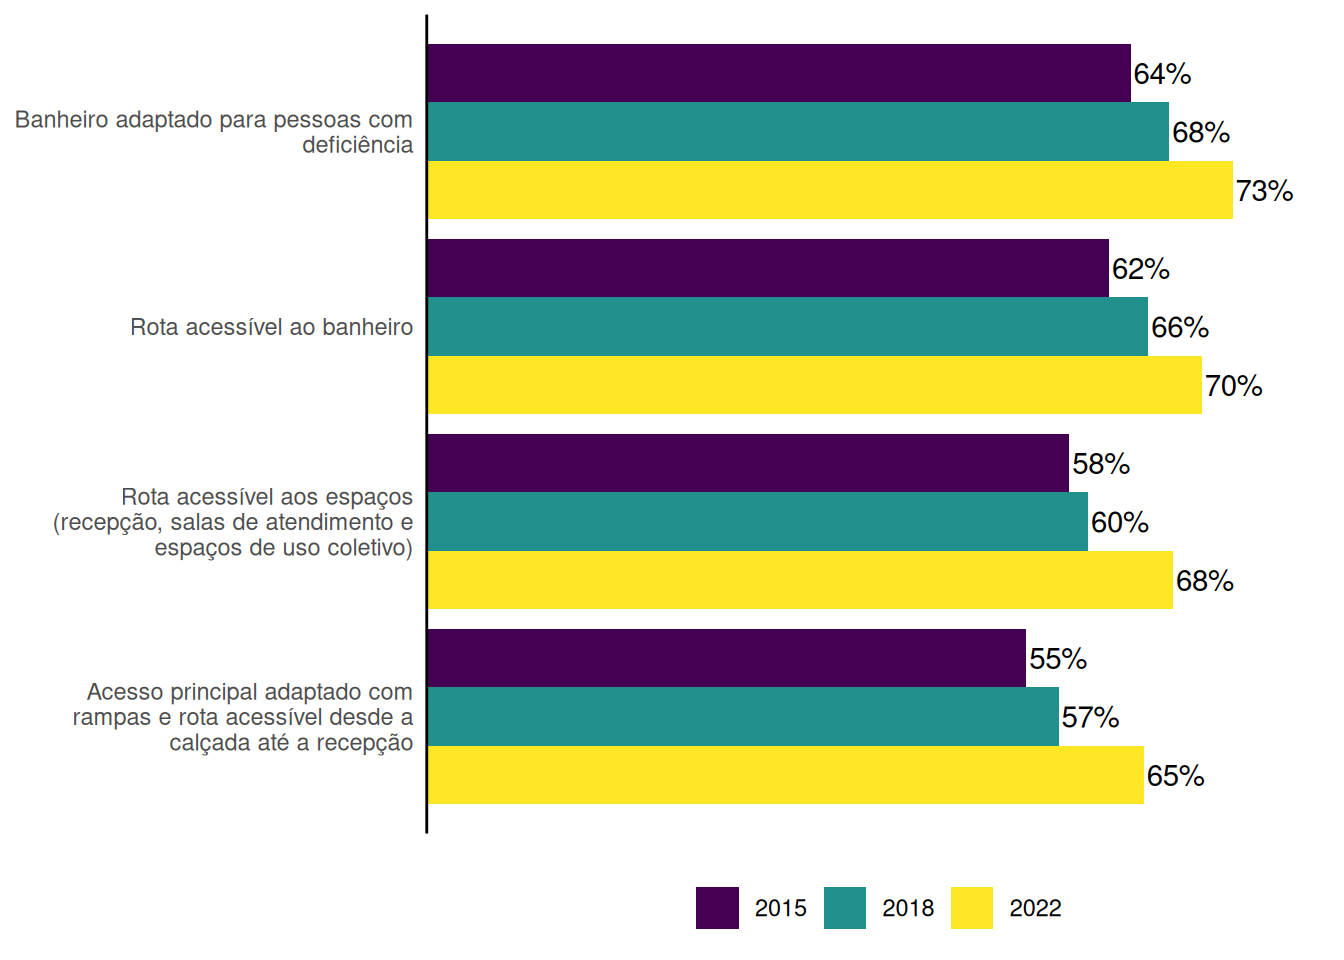
\includegraphics{unidades_files/figure-pdf/fig-cdia-acessibilidade-1.pdf}

}

\caption{\label{fig-cdia-acessibilidade}Evolução percentual de
Centro-Dia com condições de acessibilidade - Brasil; 2015, 2018 e 2022}

\end{figure}%

Além disto, há outras adaptações importantes nestas unidades, como
tecnologias assistidas, suportes com materiais em braile, profissionais
com conhecimento em Libras entre outros destacados no
Gráfico~\ref{fig-cdia_adaptacoes}.

\begin{figure}

\centering{

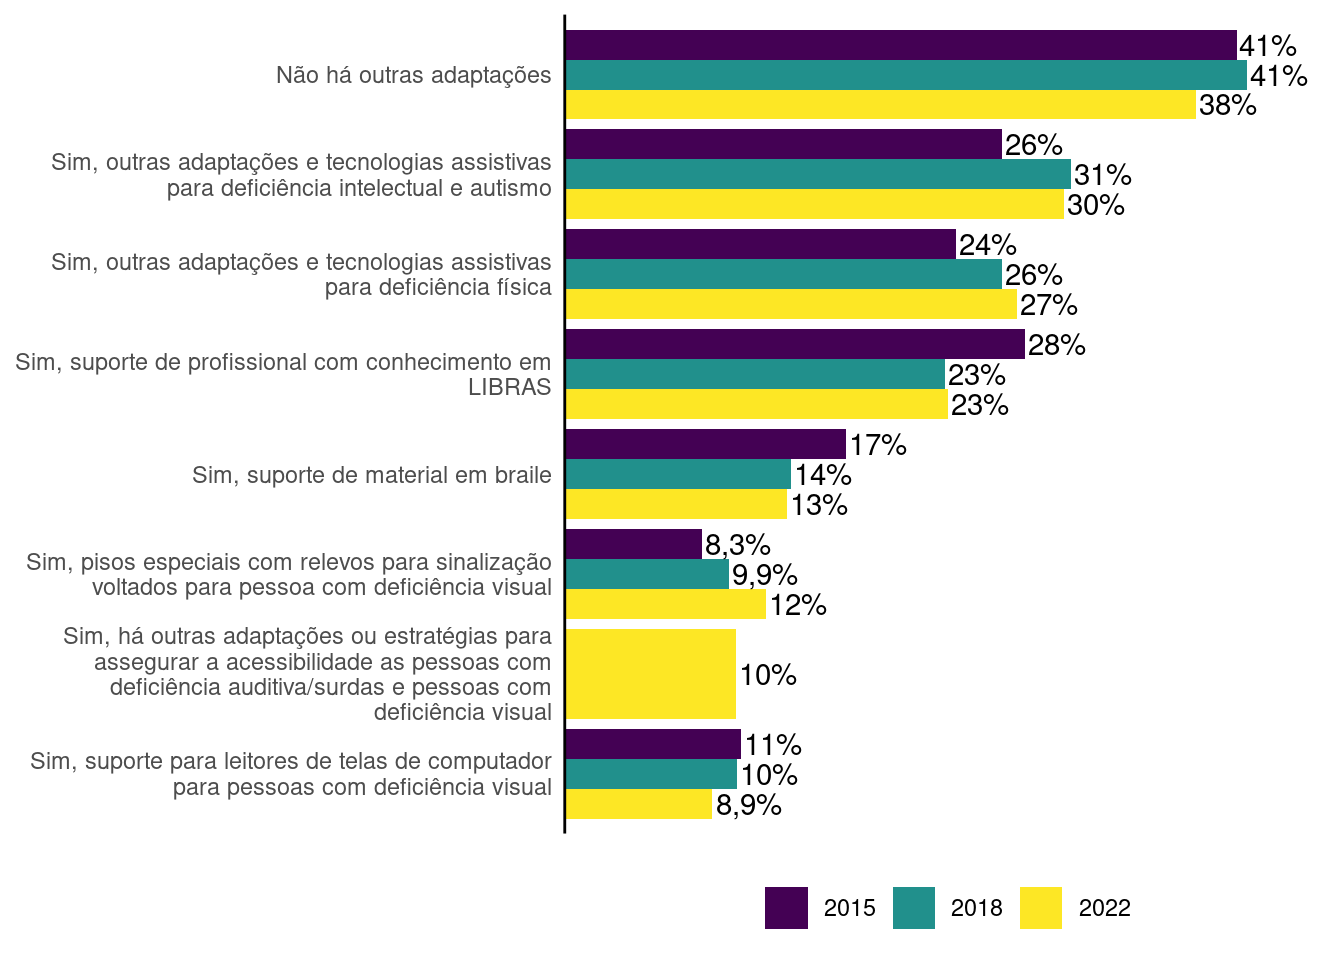
\includegraphics{unidades_files/figure-pdf/fig-cdia_adaptacoes-1.pdf}

}

\caption{\label{fig-cdia_adaptacoes}Quantidade de Centro-Dia, segundo
outras adaptações - Brasil, 2015, 2018 e 2022}

\end{figure}%

\section{Unidades de Alta
Complexidade}\label{unidades-de-alta-complexidade}

As Unidades de Acolhimento tem o objetivo de ofertar serviços de
Proteção Social Especial de Alta Complexidade, com atenção a pessoas
e/ou famílias com vínculos rompidos ou fragilizados, ou que estejam em
situação de abandono, ameaça ou violação de direitos, de forma a
garantir sua proteção integral.

No que se refere a quantidade total destas unidades de acolhimento por
porte populacional, destaca-se que há concentração nos municípios com
porte populacional maiores. Todas as metrópoles possuem registro de mais
de 10 unidades. O Gráfico~\ref{fig-unac-porte} também sinaliza que 74\%
dos municípios de pequeno porte I não dispõem de serviços de alta
complexidade.

Para os municípios menores a Resolução 31/2013 do CNAS sinaliza sobre a
oferta regionalizada e a expansão qualificada dos serviços de Alta
Complexidade para Criança e Adolescentes. O orgão gestor estadual é
responsável por esta organização.

\begin{figure}

\centering{

\includegraphics{unidades_files/figure-pdf/fig-unac-porte-1.pdf}

}

\caption{\label{fig-unac-porte}Unidades de Acolhimento e estimativas da
população para os municípios, segundo porte populacional - Brasil, 2022}

\end{figure}%

A maioria das Unidades de Acolhimento são executadas por Organizações da
Sociedade Cívil (Osc). Esse percentual teve uma redução entre 2012 e
2022. Em 2012 estes dados sinalizam percentual de 66,4\% das unidades de
acolhimento com execução de OSC, registrando em 2022 63,4\% conforme o
Gráfico~\ref{fig-acolh_nat}.

\begin{figure}

\centering{

\includegraphics{unidades_files/figure-pdf/fig-acolh_nat-1.pdf}

}

\caption{\label{fig-acolh_nat}Quantitativo de Acolhimento Institucional
por Natureza da Unidade - BRASIL, 2012 a 2022}

\end{figure}%

No que se refere às condições de acessibilidade, é possível notar
melhorias no percentual dos quatro quesitos de acessibilidade. A
adaptação mais observada é a rota acessível ao banheiro, presente em
50,9\% das Unidades, e a menos observada é o acesso principal adaptado
com rampas e rota acessível desde a calçada até o interior da unidade,
presentes em 49,2\% das Unidades. O banheiro adaptado para pessoas com
deficiência e/ou mobilidade reduzida, presente em 47,9\% das unidades em
2022 e no que se refere ao acesso principal adaptado com rampas e e rota
acessivel para o Censo SUAS 2022 observa-se presente em 45,6\% das
unidades conforme o Gráfico~\ref{fig-unac_acessibilidade}.

\begin{figure}

\centering{

\includegraphics{unidades_files/figure-pdf/fig-unac_acessibilidade-1.pdf}

}

\caption{\label{fig-unac_acessibilidade}Evolução percentual de Unidades
de Acolhimento Municipais com condições de acessibilidade - Brasil; 2017
e 2022}

\end{figure}%

Em relação ao acesso à internet, observa-se uma evolução nos últimos 10
anos. Em 2012 62,2\% das unidades possuem acesso à internet, o Censo
SUAS de 2022 destaca que 100\% dos computadores das unidades possuem
acesso à internet conforme o Gráfico~\ref{fig-unac-internet}.

\begin{figure}

\centering{

\includegraphics{unidades_files/figure-pdf/fig-unac-internet-1.pdf}

}

\caption{\label{fig-unac-internet}Percentual de Computadores nas
unidades de Acolhimento com acesso à internet, 2012, 2017 e 2022}

\end{figure}%

\section{Unidades do Cadastro
Único}\label{unidades-do-cadastro-uxfanico}

Quanto a presença das unidades do Cadastro Único, os dados do Censo SUAS
2022 sinaliza 2.892 unidades de postos do Cadastro Único conforme pode
ser observado através do Gráfico~\ref{fig-postos-cadunico}.

\begin{figure}

\centering{

\includegraphics{unidades_files/figure-pdf/fig-postos-cadunico-1.pdf}

}

\caption{\label{fig-postos-cadunico}Evolução de Postos do Cadastro Único
- 2020 - 2021 - 2022}

\end{figure}%

O Gráfico~\ref{fig-posto_cadunico} mostra o local onde estão estas
unidades. A maioria delas, 61\%, encontra-se na secretaria de
Assistência Social. A segunda proporção são postos exclusivos, com
destaque para algumas unidades presentes em escolas, conselhos e OSCS.

\begin{figure}

\centering{

\includegraphics{unidades_files/figure-pdf/fig-posto_cadunico-1.pdf}

}

\caption{\label{fig-posto_cadunico}Distribuição dos Postos do Cadastro
Único - Brasil, 2020 a 2022}

\end{figure}%

A acessibilidade nas unidades de Cadastro Único possuem leve avanço nos
últimos anos, com execeção da rota acessível aos principais espaços, os
demais itens de acessibilidade avançaram conforme pode ser observado
através do Gráfico~\ref{fig-postcad-acessibilidade}.

\begin{figure}

\centering{

\includegraphics{unidades_files/figure-pdf/fig-postcad-acessibilidade-1.pdf}

}

\caption{\label{fig-postcad-acessibilidade}Evolução percentual de postos
do Cadastro Único com condições de acessibilidade - Brasil; 2020, 2021 e
2022}

\end{figure}%

Em relação aos espaços de acessibilidade comparada a situação do imóvel,
destaca-se que os postos do Cadastro Único próprios ou cedidos, possuem
significativamente mais acessibilidade que os imóveis alugados
(Gráfico~\ref{fig-postcad-acessibilidade-situacao}).

\begin{figure}

\centering{

\includegraphics{unidades_files/figure-pdf/fig-postcad-acessibilidade-situacao-1.pdf}

}

\caption{\label{fig-postcad-acessibilidade-situacao}Percentual de Postos
do Cadastro Único com condições de acessibilidade segundo situação do
imóvel -- Brasil, 2022}

\end{figure}%

Em relação a computadores com acesso à internet, os dados do Censo SUAS
2022 sinaliza que 99\% das unidades dispõe de equipamentos com esta
estrutura, conforme pode ser observado no
Gráfico~\ref{fig-postcad-internet-percentual}.

\begin{figure}

\centering{

\includegraphics{unidades_files/figure-pdf/fig-postcad-internet-percentual-1.pdf}

}

\caption{\label{fig-postcad-internet-percentual}Evolução percentual de
Postos do Cadastro Único com computadores com acesso à internet --
Brasil; 2020, 2021 e 2022}

\end{figure}%

\section{Considerações Finais}\label{considerauxe7uxf5es-finais-1}

O Censo SUAS 2022 identificou a oferta de 30.824 unidades da Assistência
Social. São 8.557 CRAS, 7.837 Centro de Convivência, 2.846 CREAS, 33
CREAS Regionais, 237 Centro POP, 1.886 Centro-Dia, 2.892 unidades
exclusivas de Cadastro Único e 6.536 unidades de acolhimento
institucional (Crianças e adolescentes,Pessoas Idosas, Adultos e
Famílias, Pessoas com deficiência, Mulheres em situação de Violência
Doméstica, Jovens egressos serviços de acolhimento).Os dados mostram
forte presença no território nacional com destaque para crescimentonos
últimos 10 anos.

No âmbito da Proteção Básica houve um crescimento de 11\% nos últimos 10
anos. Em relação a acessibilidade há avanços, sobretudo os que possuem
imóvel próprio que chegam a ter 28 pontos percentuais de diferença em
relação aos imóveis alugados.

No que se refere a Proteção Social Especial, nos CREAS, observa-se um
crescimento de 31\% destas unidades nos últimos 10 anos. As condições de
acessibilidade dos CREAS também avança, sobretudo os que possuem imóvel
próprio com 28,4\% de diferença em relação aos imovéis alugados. Os
Centros Pop crescem 126\% ao longo dos últimos 10 anos, assim como
acessibilidade também, sobretudo para os imovéis próprios.Em relação as
Unidades de Acolhimento Institucional 45\% delas são da modalidade de
Criança e Adolescente, em seguida para públicos de Pessoas Idosas e
Adultos e Famílias. Os centros dia destacam evolução de 41\%, bem como
nas condições de acessibilidade. Para essa modalidade de oferta, 93\%
são através de OCS (Organizações da sociedade Civil).

A oferta do Cadastro Único nas unidades, em especial de CRAS avançou 3,8
pontos percentuais nos últis 10 anos, esse dado se torna
significativamente maior quando relacionado com equipe exclusiva para
esta finalidade que avança 25 pontos percentuais neste mesmo período.
Por fim, destaca-se a inclusão digital sob a ótica do acesso à internet
como algo praticamente universalizado nas unidades do SUAS.

\bookmarksetup{startatroot}

\chapter{Serviços e Benefícios ofertados pelo
SUAS}\label{serviuxe7os-e-benefuxedcios-ofertados-pelo-suas}

\section{Proteção Social}\label{proteuxe7uxe3o-social}

A Assistência Social organiza-se por dois tipos de proteção: a proteção
social básica, definida no artigo 6º-A da Lei Orgânica da Assistência
Social (LOAS) como um ``conjunto de serviços, programas, projetos e
benefícios da assistência social que visa a prevenção de situações de
vulnerabilidade e risco social por meio do desenvolvimento de
potencialidades e aquisições e do fortalecimento de vínculos familiares
e comunitários'' e a proteção social especial, definida como ``conjunto
de serviços, programas e projetos que tem por objetivo contribuir para a
reconstrução de vínculos familiares e comunitários, a defesa de direito,
o fortalecimento das potencialidades e aquisições e a proteção de
famílias e indivíduos para o enfrentamento das situações de violação de
direitos''\footnote{Lei nº 8.742, de 7 de dezembro de 1993 (Lei Orgânica
  da Assistência Social): Dispõe sobre a organização da Assistência
  Social e dá outras providências
  (\url{http://www.planalto.gov.br/ccivil_03/Leis/L8742compilado.htm}).}.

Nesse contexto, este eixo de unidades, serviços e benefícíos da
Assistência Social tem o objetivo de apresentar informações sobre a
oferta das unidades da Proteção Social Básica e Especial do SUAS
integrada aos serviços e benefícios desta política.

Para isso, os dados históricos desta publicação nos ajudam a identificar
os avanços e tendências ao longo dos anos em relação a estrutura física
destes equipamentos, oferta dos serviços e benefícios, demanda e perfis
de públicos atendidos, oferta regionalizada a partir da Resolução CIT
33/2013, integração com Cadastro Único para programas sociais, natureza
da oferta das unidades. Este conteúdo está dividido por proteções a
saber:

\begin{itemize}
\item
  \textbf{Proteção Social Básica:} PAIF (Serviço de Proteção e
  Atendimento Integral à Família), SCFV (Serviços de Convivência e
  Fortalecimento de Vínculos), Proteção Social Básica no Domicílio para
  pessoas idosas e com deficiência,
\item
  \textbf{Proteção Social Especial Média Complexidadade:} PAEFI (Serviço
  de Atendimento Especializado a Famílias e Indivíduos), Proteção Social
  Especial no Domicílio para pessoas idosas e com Deficiência, Abordagem
  Social, MSE (Medidas Socioeducativas em meio aberto), Serviço para
  situações de emergência e/ou calamidade pública.
\item
  \textbf{Proteção Social Especial Alta Complexidade:} Tipos de unidades
  de Serviço de Acolhimento Institucional, oferta de Serviços de Família
  Acolhedora, bem como do Programa de Família Guardiã ou Extensa,
  Serviço ofertado em Centro-Dia.
\end{itemize}

\section{Proteção Social Básica}\label{proteuxe7uxe3o-social-buxe1sica}

\subsection{Serviço de Proteção e Atendimento Integral à Família
(PAIF)}\label{serviuxe7o-de-proteuxe7uxe3o-e-atendimento-integral-uxe0-famuxedlia-paif}

O PAIF compõe um conjunto de ações conjugada a seguranças sociais
referenciadas a unidades de CRAS. De acordo com Tipificação Nacional dos
Serviços Socioassistenciais, o PAIF ``consiste no trabalho social com
família, de caráter continuado, com a finalidade de fortalecer a função
protetiva das famílias, prevenir a ruptura dos seus vínculos, promover
seu acesso e usufruto do direito'' \footnote{Resolução nº 109/2009 /
  CNAS}.

A respeito das principais ações desenvolvidas no âmbito do PAIF,
destaca-se que as três atividades mais realizadas pelas unidades são
visitas domiciliares, encaminhamento para o Cadastro Único e acolhida
particularizada. .

\subsection{Serviços de Convivência e Fortalecimento de Vínculos
(SCFV)}\label{serviuxe7os-de-convivuxeancia-e-fortalecimento-de-vuxednculos-scfv}

A tônica do vínculo é um fator de Segurança Social. O SCFV no âmbito do
SUAS é um serviço tipificado e realizado através de grupos na qual
objetiva garantir aquisições progressivas aos cidadãos usuários do SUAS.
Trata-se de serviço que afirma da natureza relacional no processo de
proteção e complementar ao trabalho social com família e atua de forma
preventiva a ocorrências de situações de risco social. De acordo com o
Gráfico~\ref{fig-CRAS-SCFV}, 82\% dos CRAS possuem a oferta deste
serviço na sua unidade. Há também esta oferta por meio de Unidades de
Centro de Convivência conforme já mencionado.

\begin{figure}

\centering{

\includegraphics{servicos_files/figure-pdf/fig-CRAS-SCFV-1.pdf}

}

\caption{\label{fig-CRAS-SCFV}Percentual de CRAS que executavam
diretamente os Serviços de Convivência e Fortalecimento de Vínculos -
Brasil, 2014 a 2022}

\end{figure}%

Dos 2.334 CRAS que informaram que havia povos e comunidades tradicionais
em seu território de abrangência, 896 informaram ter atendido
Comunidades Quilombolas (38,4\%), seguidos por 615 CRAS que informaram
ter atendido Comunidades Ribeirinhas (26,3\%) e 611 que informaram ter
atendido Povos Indígenas (26,2\%) (Gráfico 27).

\subsection{Serviços de Proteção Social Básica no domicílio para Pessoas
Idosas e com
Deficiência}\label{serviuxe7os-de-proteuxe7uxe3o-social-buxe1sica-no-domicuxedlio-para-pessoas-idosas-e-com-deficiuxeancia}

Os Serviços de Proteção Social Básica no domicílio para Pessoas Idosas e
com Deficiência estão previstos na Tipificação dos Serviços
Socioassistenciais. Recentemente a Resolução CNAS Nº 117/2023 atualizou
a tipificação, incluindo crianças e gestantes como público alvo da
modalidade destes serviços.\footnote{RESOLUÇÃO CNAS/MDS Nº 117, DE 28 DE
  AGOSTO DE 2023}. Os dados do Gráfico~\ref{fig-CRAS-PSB} mostram um
aumento de 3 pontos percentuais no período de 2018 a 2022.\footnote{essa
  pergunta surge a partir de 2018}. Atualmente 73\% das unidades
informam possuir a oferta destes serviços.

\begin{figure}

\centering{

\includegraphics{servicos_files/figure-pdf/fig-CRAS-PSB-1.pdf}

}

\caption{\label{fig-CRAS-PSB}Percentual de CRAS que executavam
diretamente os Serviços de Proteção Social Básica nos domicílios -
Brasil, 2014 a 2022}

\end{figure}%

\section{Proteção Social Especial}\label{proteuxe7uxe3o-social-especial}

\subsection{Serviços de Proteção Social Especial -- Média
Compexidade}\label{serviuxe7os-de-proteuxe7uxe3o-social-especial-muxe9dia-compexidade}

A Proteção Social Especial de Média Complexidade organiza a oferta de
serviços, programas e projetos de caráter especializado que requerem
maior estruturação técnica e operativa, com competências e atribuições
definidas, destinados ao atendimento a famílias e indivíduos em situação
de risco pessoal e social, por violação de direitos.

É ofertada pelos Centros de Referência Especializados de Assistência
Social (CREAS), pelos Centros de Referência Especializados para
População em Situação de Rua (Centro POP), e pelos Centro-Dia. No nível
de Média Complexidade, são ofertados o Serviço de Proteção e Atendimento
Especializado a Famílias e Indivíduos (PAEFI); o Serviço de Proteção
Social a Adolescentes em Cumprimento de Medida Socioeducativa de
Liberdade Assistida e de Prestação de Serviços à Comunidade; o Serviço
Especializado em Abordagem Social; o Serviço de Proteção Social Especial
para Pessoas com Deficiência, Idosos e suas Famílias e o Serviço
Especializado para Pessoas em Situação de Rua.

\subsection{Serviço de Proteção e Atendimento e Atendimento
Especializado a Famílias e Indivíduos
(PAEFI)}\label{serviuxe7o-de-proteuxe7uxe3o-e-atendimento-e-atendimento-especializado-a-famuxedlias-e-indivuxedduos-paefi}

O PAEFI é definido na Tipificação Nacional de Serviços
Socioassistenciais como sendo o ``serviço de apoio, orientação e
acompanhamento a famílias com um ou mais de seus membros em situação de
ameaça ou violação de direitos. Compreende atenções e orientações
direcionadas para a promoção de direitos, a preservação e o
fortalecimento de vínculos familiares, comunitários e sociais e para o
fortalecimento da função protetiva das famílias diante do conjunto de
condições que as vulnerabilizam e/ou as submetem a situações de risco
pessoal e social.''

Essa seção se dedica a identificar as situações atendidas pelo PAEFI em
relação aos as situações de violências e violações de direitos
relacionadas aos ciclos de vida, trabalho, gênero e discriminações por
raça e etnia e situações de pessoas com deficiência. \footnote{todos os
  gráficos são a partir do ano de 2019 em decorrência do início da
  modalidade da pergunta no formulário do Censo SUAS}

O Gráfico~\ref{fig-paefi_creas} mostra que os principais atendimentos,
entre o período de 2019 a 2022, são os seguintes: abuso e violência
sexual, violência contra mulher, crianças e adolescentes, situações de
negligência e abandono.

\begin{figure}

\centering{

\includegraphics{servicos_files/figure-pdf/fig-paefi_creas-1.pdf}

}

\caption{\label{fig-paefi_creas}Atendimentos realizados pelo PAEFI/CREAS
por situações de riscos em decorrência de situações e ciclos de vida -
Brasil 2022}

\end{figure}%

Em relação a violação decorrente de trabalho análogo a escravidão é
definida como toda atividade forçada desenvolvida sob condições
degradantes ou em jornadas exaustivas e quando a pessoa é impedida de
deixar o seu local de trabalho \footnote{Artigo 149 do Código Penal}. O
Gráfico~\ref{fig-paefi2_creas} também traz as situações de trabalho
infantil. Observa-se que a maior demanda atendida pelos CREAS, entre o
período de 2020 e 2022,\footnote{esse gráfico é a partir do ano de 2020
  em decorrência do início da pergunta no formulário do Censo SUAS}
através do PAEFI é trabalho infantil presente em 68\% dos CREAS.
Entretanto as situações de situações de trabalho análogo a escravidão é
presente em média 13\% dos CREAS.

\begin{figure}

\centering{

\includegraphics{servicos_files/figure-pdf/fig-paefi2_creas-1.pdf}

}

\caption{\label{fig-paefi2_creas}Atendimentos realizados pelo
PAEFI/CREAS por situações de riscos em decorrência trabalho análogo a
escravidão e trabalho infantil - Brasil 2022}

\end{figure}%

As situações de imigração / refúgio vem crescendo no âmbito das demandas
do PAEFI, os dados do período de 2020 e 2022\footnote{esse gráfico é a
  partir do ano de 2020 em decorrência do início da pergunta no
  formulário do Censo SUAS} (Gráfico~\ref{fig-paefi6_creas}) sinaliza
que todos os públicos aumentam ao longo destes dois anos.

\begin{figure}

\centering{

\includegraphics{servicos_files/figure-pdf/fig-paefi6_creas-1.pdf}

}

\caption{\label{fig-paefi6_creas}Atendimentos realizados pelo
PAEFI/CREAS - Pessoas em situação de imigração / refúgio - Brasil 2022}

\end{figure}%

No que se refere ao atendimento de violências e violações a povos e
comunidades tradicionais o Gráfico~\ref{fig-creas-tradicionais}
destaca-se que dos seis povos e comunidades destacadas, as maiores
demandas estão para os públicos de comunidades quilombolas com 36\%,
povos indígenas com 35\% e ribeirinhos com 29\%.

As regiões Sul e Centro Oeste possuem maior demanda de atendimento do
público povos indígenas sendo respectivamente 72\% e 59\%
respectivamente. A região Nordeste se destaca com atendimento de
comunidades quilombolas com 55\% e a Região Norte com 74\% de demandas
de comunidades ribeirinhas.

\begin{figure}

\centering{

\includegraphics{servicos_files/figure-pdf/fig-creas-tradicionais-1.pdf}

}

\caption{\label{fig-creas-tradicionais}Percentual de CREAS que atendem
povos e comunidades tradicionais - por grupos , Região - 2022}

\end{figure}%

\subsection{Serviço de Proteção Social a Adolescentes em Cumprimento de
Medida Socioeducativa de Liberdade Assistida (LA) e de Prestação de
Serviços à Comunidade
(PSC)}\label{serviuxe7o-de-proteuxe7uxe3o-social-a-adolescentes-em-cumprimento-de-medida-socioeducativa-de-liberdade-assistida-la-e-de-prestauxe7uxe3o-de-serviuxe7os-uxe0-comunidade-psc}

O Serviço de Proteção Social a Adolescentes em Cumprimento de Medida
Socioeducativa de Liberdade Assistida (LA) e de Prestação de Serviços à
Comunidade (PSC), segundo definido na Tipificação Nacional de Serviços
Socioassistenciais, ``tem por finalidade prover atenção
socioassistencial e acompanhamento a adolescentes e jovens em
cumprimento de medidas socioeducativas em meio aberto, determinadas
judicialmente. Deve contribuir para o acesso a direitos e para a
resignificação de valores na vida pessoal e social dos adolescentes e
jovens. Para a oferta do serviço faz-se necessário a observância da
responsabilização face ao ato infracional praticado, cujos direitos e
obrigações devem ser assegurados de acordo com as legislações e
normativas específicas para o cumprimento da medida.

Em 2017, 81\% dos municípios ofertavam o Serviço de Medidas
Socioeducativas em Meio Aberto (MSE) de Liberdade Assistida (LA) e
Prestação de Serviço à Comunidade (PSC) através dos CREAS. Esse
percentual aumentou nos últimos anos, conforme pode ser observado no
Gráfico~\ref{fig-CREAS-MSE}. O aumento foi de 8 pontos percentuais. O
Censo SUAS de 2022 mostra que 89\% dos CREAS ofertam este serviço. O
principal objetivo desta oferta é assegurar a função protetiva destes
jovens em situação de cumprimento de MSE e suas respectivas famílias em
conjunto com Sistema de Garantias de Direitos (SGC).

\begin{figure}

\centering{

\includegraphics{servicos_files/figure-pdf/fig-CREAS-MSE-1.pdf}

}

\caption{\label{fig-CREAS-MSE}Percentual de CREAS que realizam o Serviço
de Proteção Social a Adolescentes em cumprimento de Medida
Socioeducativa de Liberdade Assistida (LA) e de Prestação de Serviços à
Comunidade (PSC) - Brasil, 2017 a 2022}

\end{figure}%

\subsection{Serviço de Proteção Social Especial para Pessoas com
Deficiência e Pessoas Idosas e suas
famílias}\label{serviuxe7o-de-proteuxe7uxe3o-social-especial-para-pessoas-com-deficiuxeancia-e-pessoas-idosas-e-suas-famuxedlias}

O Serviço de Proteção Social Especial para Pessoas com Deficiência e
Pessoas Idosas e suas famílias é definido na Tipificação Nacional de
Serviços Socioassistenciais como sendo o ``serviço para a oferta de
atendimento especializado a famílias com pessoas com deficiência e
idosos com algum grau de dependência, que tiveram suas limitações
agravadas por violações de direitos, tais como: exploração da imagem,
isolamento, confinamento, atitudes discriminatórias e preconceituosas no
seio da família, falta de cuidados adequados por parte do cuidador, alto
grau de estresse do cuidador, desvalorização da
potencialidade/capacidade da pessoa, dentre outras que agravam a
dependência e comprometem o desenvolvimento da autonomia.''

No que se refere às ações e atividades no âmbito do CREAS\footnote{gráficos
  são a partir do ano de 2018 em decorrência do início da modalidade da
  pergunta no formulário do Censo SUAS}, o
Gráfico~\ref{fig-creas-pse-domicilio} mostra redução na quantidade de
Serviço de Proteção Social Especial para Pessoas com Deficiência e
Pessoas Idosas com equipe específica para sua execução. Em concomitante,
aumenta a oferta sem equipe exclusiva. Os dados também destacam que há
redução em relação aos municípios que deixam de ofertar este serviços
que vai de 20\% em 2018 para 31\% em 2022. Outro movimento é o aumento
dos municípios que realizam a oferta do serviço em outra unidade além do
CREAS.

\begin{figure}

\centering{

\includegraphics{servicos_files/figure-pdf/fig-creas-pse-domicilio-1.pdf}

}

\caption{\label{fig-creas-pse-domicilio}Percentual de CREAS que realizam
Serviço de Proteção Social Especial para Pessoas com Deficiência, Idosas
e suas Famílias, 2018 a 2022}

\end{figure}%

\subsection{Serviço Especializado em Abordagem
Social}\label{serviuxe7o-especializado-em-abordagem-social}

O Serviço Especializado em Abordagem Social consiste na identificação,
por equipes de educadores sociais, de pessoas e famílias em situação de
risco pessoal nos ambientes públicos. Dentre as situações de risco
enquadram-se o trabalho infantil, situação de rua, uso abusivo de
drogas, exploração sexual de crianças e adolescentes, dentre outras. A
abordagem é realizada em praças, feiras, locais de intensa circulação de
pessoas e com existência de comércio, ruas, prédios abandonados, dentre
outros espaços, e tem por objetivo garantir direitos por meio de
inclusão em rede de serviços socioassistenciais e em outras políticas
públicas.

No Gráfico~\ref{fig-CREAS-abordagem-social}\footnote{gráfico a partir do
  ano de 2018 em decorrência do início da modalidade da pergunta no
  formulário do Censo SUAS} observa-se uma redução da oferta deste
serviço entre o período de 2018 a 2022. Os dados sinalizam que aumenta o
número de CREAS que deixam de ofertar este serviço nesta unidade, esse
evolui de 14\% para 17\% das unidades. O número de municípios que deixam
de ofertar este serviços também aumenta de 20\% para 31\%. Concomitante
a estas informações, reduz-se o número de municípios que ofertam, seja
com equipe ou sem equipe exclusiva para execução dos serviços.

\begin{figure}

\centering{

\includegraphics{servicos_files/figure-pdf/fig-CREAS-abordagem-social-1.pdf}

}

\caption{\label{fig-CREAS-abordagem-social}Quantidade de CREAS que
realizam o Serviço Especializado em Abordagem Social, 2018 - 2020 e
2022}

\end{figure}%

\section{Proteção Social Especial de Alta
Complexidade}\label{proteuxe7uxe3o-social-especial-de-alta-complexidade}

Os Serviços de Proteção Social Especial de Alta Complexidade destinam-se
a famílias e/ou indivíduos afastados temporariamente do núcleo familiar
e/ou comunitário de origem. Estes Serviços são organizados em diferentes
regulamentações, modalidades e públicos. Os públicos dos serviços
tipificados são:

\begin{itemize}
\tightlist
\item
  \textbf{Crianças e Adolescentes:} Unidade residencial e unidades
  institucional
\item
  \textbf{Pessoas Idosas:} Unidade residencial e unidades institucional
\item
  \textbf{Adultos e famílias:} Unidade residencial tipo de residência e
  unidade institucional e passagem
\item
  \textbf{Jovens e Adultos com deficiência:} residência Inclusiva
\item
  \textbf{Mulheres:} Unidade residencial
\end{itemize}

\subsection{Serviço de Acolhimento em Família
Acolhedora}\label{serviuxe7o-de-acolhimento-em-famuxedlia-acolhedora}

O Serviço de Acolhimento em Família Acolhedora ``organiza o acolhimento
de crianças e adolescentes, afastados da família por medida de proteção,
em residência de famílias acolhedoras cadastradas. É previsto até que
seja possível o retorno à família de origem ou, na sua impossibilidade,
o encaminhamento para adoção. O serviço é o responsável por selecionar,
capacitar, cadastrar e acompanhar as famílias acolhedoras, bem como
realizar o acompanhamento da criança e/ou adolescente acolhido e sua
família de origem.''

No território Nacional há 54\% dos municípios informam que possuem este
serviço conforme dados de 2022. Essa proporção cresceu em relação ao ano
de 2017, conforme pode ser observado no
Gráfico~\ref{fig-fam_acolhedora}. O gráfico também referencia a oferta
destes serviços por grandes regiões, as regiões Sul e Sudeste se
destacam como o maior número quantitativo e a Região Nordeste em termos
de crescimento proporcional neste período. AS regiões Centro Oeste e
Norte foram as que menos tiveram crescimento da oferta do Serviço de
Acolhimento em Família Acolhedora no âmbito dos municípios.

.

\begin{figure}

\centering{

\includegraphics{servicos_files/figure-pdf/fig-fam_acolhedora-1.pdf}

}

\caption{\label{fig-fam_acolhedora}Percentual de municípios com Serviços
de Família Acolhedora - Região, 2017 a 2022}

\end{figure}%

.

\section{Benefícios Eventuais}\label{benefuxedcios-eventuais}

Os Benefícios Benefícios Eventuais, são previsões do SUAS e suas ofertas
devem ser garantidas ``em sua integralidade -- benefícios, serviços e
programas -- de forma que a capacidade protetiva do Estado seja
efetivada de forma a fortalecer a autonomia das famílias, garantindo os
encaminhamentos necessários''. \footnote{Orientações técnicas sobre
  Benefícios Eventuais no SUAS, acesso através:
  https://www.sigas.pe.gov.br/files/01282019120030-orientacoes.tecnias.sobre.beneficios.eventuais.no.suas.pdf}

São concedidos em casos de nascimento, morte, situações de
vulnerabilidade provisória e de calamidade pública.

Destaca-se que a oferta deste Benefício Eventual caracteriza-se como um
direito, portanto diferencia-se de doação. A forma e critérios desta
oferta devem ser deliberadas pelo Conselho de Assistência Social local.

Dados de 2022 informa que 98\% dos municípios concedem este Benefício
Eventual para situações de Vulerabildiade temporária e de Morte. Em
seguida, 90\% dos entes municipais informam para situações de calamidade
pública e 87\% dos municípios em situação de natalidade conforme o
Gráfico~\ref{fig-be-munic}.

\begin{figure}

\centering{

\includegraphics{servicos_files/figure-pdf/fig-be-munic-1.pdf}

}

\caption{\label{fig-be-munic}Percentual de municípios que concedem
Benefícios Eventuais - 2022}

\end{figure}%

Em relação ao local da oferta destes Benefícios Eventuais, destaca-se no
Gráfico~\ref{fig-be-local} que há três locais descritos pelos gestores
municipais, são eles: oferta na sede do orgão gestor, oferta nas
unidades da rede socioassistencial e, em ambos. Para as situações de
morte, os dados apontam que 40\% desta oferta é realizada no orgão
gestor municipal. Em caso de nascimento e situação de vulnerabilidade
temporária a maior proporção encontra-se nas unidades da rede
socioassistencial com 42\% e 37\% respectivamente.

\begin{figure}

\centering{

\includegraphics{servicos_files/figure-pdf/fig-be-local-1.pdf}

}

\caption{\label{fig-be-local}Percentual de local onde os benefícios
eventuais são concedidos nos municípios - 2022}

\end{figure}%

\section{Considerações Finais}\label{considerauxe7uxf5es-finais-2}

Os dados do Censo SUAS 2022 sinaliza que ações como visitas
domiciliares, encaminhamento para inserção/atualização e acolhida
particularizada são as principais ações realizadas pelos PAIF sendo a
primeira em 100\% das unidades de serviços. Atendimento em comunidades
tradicionais se destaca com especificidades regionais no Censo SUAS
2022. Dois públicos são hegemonicamente, para regiões Nordeste, Sudeste
e Sul são as comunidades quilombolas e para as regiões Norte e Centro
Oeste os públicos de comunidades ribeirinhas são proporcionalmente mais
presentes nos atendimentos dos PAIF nos CRAS.

Em relação a oferta de SCFV, os dados sinalizam que 82\% dos CRAS
ofertam diretamente este serviço. Dado que cresceu em relação aos dois
últimos anos do censo, entretanto comparado a partir de 2014, teve
redução de 7 pontos percentuais. Já o Serviço de Proteção Social Básica
no Domicílio, é um dado que decresceu ao longo dos últimos 4 anos. O
último Censo SUAS sinaliza que 27\% dos CRAS ofertam este serviço em
domicílio.

Na Proteção Social Especial através do PAEFI, destaca-se que violência
contra criança e adolescentes e contra mulher são as demandas mais
presentes no âmbito do PAEFI. Em relação a violações, o trabalho
infantil é presente em 68\% dos atendimentos dos CREAS. No aspecto
migratório, essa demanda aumento nos últimos anos, sobre tudo no perfil
de pessoas adultas (homens e mulheres).

Em relação ao atendimento de povos e comunidades tradicionais netas
unidades, destaca-se que os dados variam conforme região, sendo
hegemonicamente mais presente os públicos de comunidades quilombolas,
povos indígenas e ribeirinhos. A oferta de Serviços de MSE em meio
aberto pelos CREAS cresceu nos últimos anos 8 pontos percentuais. Já o
Serviço PSE para Pessoas com deficiência e idosas diminuiu nos últimos 4
anos, chegando em 2022 com 31\% dos municípios que não é realizado nem
pelo CREAS, nem em nenhuma outra unidade no município. O Serviços de
abordagem social também reduz nos últimos 4 anos, chegando a 31\% dos
municípios que não realiza no CREAS e não possui em nenhumas outras
unidades do município.

No que se refere a proteção social especial de alta complexidade,
destaca-se aumento nos municípios que informam ofertar serviço de
família acolhedora, atualmente 54,3\% dos municípios informam realizar
esta oferta, dado que cresceu 27 pontos percentuais de 2017 até 2022.

No que se refere a oferta de Benefícios Eventuais, dados de 2022
informam que a maior concessão nos municípios é para situações de
vulnerabilidade temporária e de morte (98\% dos municípios). Sobre o
local da oferta eles variam, sendo que na oferta por situação de morte a
maior proporção é no órgão gestor da política de Assistência Social, com
40\% dos municípios que ofertam. Benefícios eventuais em situação de
vulnerabilidade temporária e natalidade está mais presente na rede
socioassistencial, com 37\% e 42\% respectivamente. 34\% dos municípios
informam ofertar benefícios em situação de calamidade pública pelo órgão
gestor, e este mesmo percentual (34\%) de municípios informa ofertar em
unidades da rede socioassistencial.

\bookmarksetup{startatroot}

\chapter{Gestão do Trabalho e Recursos Humanos no
SUAS}\label{gestuxe3o-do-trabalho-e-recursos-humanos-no-suas}

A qualidade da oferta de serviços, programas e benefícios da assistência
social está diretamente ligada a uma adequada gestão do trabalho no
âmbito do SUAS. O dimensionamento das equipes, a capacitação dos
profissionais e a estruturação das condições de trabalho são
fundamentais nesse sentido. Um importante normativo para a gestão do
trabalho é Norma Operacional Básica de Recursos Humanos do SUAS
(NOB-RH/SUAS), que traz orientações e diretrizes, além de detalhamentos
importantes sobre as equipes de referência, planos de carreira, cargos e
salários, cofinanciamento, educação permanente, entre outros aspectos
relevantes. A NOB SUAS 2012 em seu capítulo VIII também descreve sobre a
Gestão do Trabalho no SUAS no âmbito da União, dos Estados, do Distrito
Federal e dos Municípios. \footnote{acesso
  através:\url{https://www.mds.gov.br/webarquivos/public/NOBSUAS_2012.pdf}}

Esta seção apresenta um panorama geral da situação das trabalhadoras e
trabalhadores do SUAS, tanto nos equipamentos da assistência social
quanto nas gestões municipais e estaduais, apresentando informações
sobre quantitativo, tipo de vínculo trabalhista, escolaridade, entre
outros aspectos referentes à gestão do trabalho, e sua evolução ao longo
dos anos.

\section{Evolução na quantidade de trabalhadoras/es, tipo de vínculo e
escolaridade no orgão
gestor}\label{evoluuxe7uxe3o-na-quantidade-de-trabalhadorases-tipo-de-vuxednculo-e-escolaridade-no-orguxe3o-gestor}

A quantidade de trabalhadoras/es nas Secretarias Estaduais de
Assistência Social nacionalmente em 2018\footnote{gráfico a partir do
  ano de 2018 em decorrência de mudanças na modalidade de respostas} era
de 3.988 profissionais, considerando trabalhadoras/es lotadas/os na sede
do órgão gestor. Esse quantitativo teve aumento 7\%, em 2022 passou a
ter 4.265 conforme pode ser observado no Gráfico~\ref{fig-qtd-trab-uf}.

\begin{figure}

\centering{

\includegraphics{rh_files/figure-pdf/fig-qtd-trab-uf-1.pdf}

}

\caption{\label{fig-qtd-trab-uf}Evolução da quantidade de
trabalhadoras/es nas Secretarias Estaduais de Assistência Social -
Brasil e grandes regiões, 2018 a 2022}

\end{figure}%

A quantidade de trabalhadoras/es nas Secretarias Municipais de
Assistência Social em 2018\footnote{gráfico a partir do ano de 2018 em
  decorrência de mudanças na modalidade de respostas} era de 51.135
profissionais, considerando trabalhadoras/es lotados na sede do órgão
gestor. Esse quantitativo aumento 4\%, em 2022 passou a ter 56.381
conforme pode ser observado no Gráfico~\ref{fig-qtd_trab_munic}.

\begin{figure}

\centering{

\includegraphics{rh_files/figure-pdf/fig-qtd_trab_munic-1.pdf}

}

\caption{\label{fig-qtd_trab_munic}Evolução da quantidade de
trabalhadoras/es nas Secretarias Municipais de Assistência Social -
Brasil, 2018 a 2022}

\end{figure}%

O Gráfico~\ref{fig-uf_trab_vin} traz dados sobre o tipo de vínculo dos
trabalhadores e trabalhadoras das Secretarias Estaduais de Assistência
Social. Observa-se uma redução das/os servidoras/es estatutárias/os e
empregadas/os públicos (CLT). O percentual de Servidoras/es caem de 54\%
no ano de 2012 para 46\% em 2022. Enquanto empregadas/os públicas/os
reduzem de 16\% em 2012 para 3,3\% em 2022. Houve aumento de cargos
comissionados 10 pontos percentuais, de 19\% em 2012 para 29\% em 2022.

\begin{figure}

\centering{

\includegraphics{rh_files/figure-pdf/fig-uf_trab_vin-1.pdf}

}

\caption{\label{fig-uf_trab_vin}Percentual de trabalhadoras/es nas
Secretarias Estaduais de Assistência Social, segundo tipo de vínculo -
Brasil, 2012, 2017 e 2022}

\end{figure}%

Os percentuais de trabalhadoras/es segundo tipo de vínculo pode ser
observados no Gráfico~\ref{fig-munic_trab_vin}. A quantidade
proporcional de estatutários na gestão municipal representavam 36\% em
2013,\footnote{não foi possível gerar este gráficos para os anos de 2012
  e 2020 em decorrência de problemas na leitura da base de dados do
  Censo SUAS} observa-se um aumento no ano de 2017 e retoma ao patamar
de 36\% em 2022.

Este gráfico também sinaliza uma significativa diminuição no público de
empregadores públicos que representa 11\% das/os trabalhadoras/es no ano
de 2013 e reduz para 4,7\% em 2022. Dados de outros vínculos não
permanente também reduz de 37\% em 2013 para 29\% no ano de 2022. O
único dado percentual que eleva nas gestões dos municípios são
referentes a cargos comissionados. Este dados avança de 17\% em 2013
para 31\% em 2022.

Destaca-se que em outros vínculos não permanentes estão incluídos
voluntários.

\begin{figure}

\centering{

\includegraphics{rh_files/figure-pdf/fig-munic_trab_vin-1.pdf}

}

\caption{\label{fig-munic_trab_vin}Percentual de trabalhadoras/es nas
Secretarias Municipais de Assistência Social, segundo tipo de vínculo -
Brasil, 2013, 2017 e 2022}

\end{figure}%

Quanto a escolaridade das/os trabalhadoras/es das Secretarias Estaduais
de Assistência Social observa-se um aumento significativo dos
profissionais de nível superior com avanço de 32\% em 2012 para 63\% em
2022. Em relação reduz o número proporção de profissionais de nível
fundamental e médio. A soma deste grupo representava 68\% em 2012 e
chega em 2022 com 37,2\% conforme pode ser analisada através do
Gráfico~\ref{fig-uf_trab_form}.

\begin{figure}

\centering{

\includegraphics{rh_files/figure-pdf/fig-uf_trab_form-1.pdf}

}

\caption{\label{fig-uf_trab_form}Percentual de trabalhadoras/es nas
Secretarias Estaduais de Assistência Social, segundo escolaridade -
Brasil; 2012, 2017 e 2022}

\end{figure}%

O Gráfico~\ref{fig-munic_trab_form} mostra a evolução do número de
trabalhadoras/es de nível superior, ele avança de 36\% para 52\% no
período de 2013 \footnote{não foi possível gerar este gráficos para os
  anos de 2012 e 2020 em decorrência de problemas na leitura da base de
  dados do Censo SUAS} a 2022. Em relação a propoção de profissionais de
nível médio e fundamental, há uma redução ao longo deste período com 6,3
pontos percentuais para de nível fundamental e 10 pontos percentuais
para profissionais de nível médio. Assim, o Censo SUAS de 2022 sinaliza
que, do total de trabalhadoras/es na gestão municipal, há 39\% de nível
fundamental e 8,7\% de nível médio. Demais 52\%, correspondem a
profissionais de nível superior.

\footnote{não foi possível gerar este gráficos para os anos de 2012 e
  2020 em decorrência de problemas na geração dos dados}.

\begin{figure}

\centering{

\includegraphics{rh_files/figure-pdf/fig-munic_trab_form-1.pdf}

}

\caption{\label{fig-munic_trab_form}Percentual de trabalhadoras/es nas
Secretarias municipais, segundo escolaridade - Brasil, 2013 a 2022}

\end{figure}%

Das/os trabalhadoras/es das Secretarias Estaduais de Assistência Social
que informaram sua formação superior em 2022, destaca-se a maior
presença de profissionais de serviços social com 24\%, após
identifica-se a proporção de profissionais de psicologia com 8,2\%. O
maior número de profissionais são identificados em outras profissões ou
não informado.\footnote{O número elevado da categoria de ``outro
  profissional não informado'' se deve a soma na base de dados nas
  informações de outros profissionais de nível superior a profissionais
  ``sem formação profissional''. Entretanto, pela relevância desta
  informação mantemos o gráfico.}

\begin{figure}

\centering{

\includegraphics{rh_files/figure-pdf/fig-uf_trab_prof-1.pdf}

}

\caption{\label{fig-uf_trab_prof}Percentual de trabalhadoras/es de nível
superior nas Secretarias Estaduais de Assistência Social, segundo área
de formação - Brasil; 2012, 2017 e 2022}

\end{figure}%

\begin{figure}

\centering{

\includegraphics{rh_files/figure-pdf/fig-munic_trab_prof-1.pdf}

}

\caption{\label{fig-munic_trab_prof}Percentual de trabalhadoras/es nas
Secretarias municipais de Assistência Social, segundo área de formação -
Brasil; 2013, 2017 e 2022}

\end{figure}%

\section{Evolução da quantidade de trabalhadoras/es nas Unidades do
SUAS}\label{evoluuxe7uxe3o-da-quantidade-de-trabalhadorases-nas-unidades-do-suas}

O Artigo 6º da Lei Orgânica de Assistência Social (LOAS) estabelece que
os recursos do cofinanciamento do SUAS poderão ser aplicados no
pagamento dos profissionais que integrarem as equipes de referência. Os
dados do Censo SUAS 2022 sinalizam um total de 145.861 trabalhadoras/es
sendo 115.149 CRAS, 27.084 CREAS e 36.628 Centro POP.

O Gráfico~\ref{fig-trab-unidades} mostra um aumento na quantidade de
trabalhadoras/es nas unidades socioassistenciais no período de 2012 a
2022. Essa evolução neste período representa 69\% nos CRAS, 36\% nos
CREAS, 122\% no Centro POP.

\begin{figure}

\centering{

\includegraphics{rh_files/figure-pdf/fig-trab-unidades-1.pdf}

}

\caption{\label{fig-trab-unidades}Evolução da quantidade de
trabalhadoras/es dos CRAS, CREAS e Centro POP - Brasil; 2012, 2017 e
2022}

\end{figure}%

.

\section{Gestão do trabalho: Concurso
público}\label{gestuxe3o-do-trabalho-concurso-puxfablico}

A gestão do trabalho no SUAS compreende desenhos organizativos,
avaliação de desempenho, adequação de perfis profissionais ás
necessidades das areas administrativas, mesas de negociação, plano de
carreira e previsão de consursos públicos.

Em relação a realização de concursos públicos pelos entes estaduais, o
Gráfico~\ref{fig-conc_estado} mostra a linha histórica quanto a
realização de concurso para trabalhadoras/es de nível superior do SUAS.
Por pelos menos 5 anos neste período, nenhum estado realizadou concurso
para nível superior no SUAS.

\begin{figure}

\centering{

\includegraphics{rh_files/figure-pdf/fig-conc_estado-1.pdf}

}

\caption{\label{fig-conc_estado}Percentual de estados que realizaram
concursos para trabalhadores nível superior do SUAS - Brasil, 2013 a
2022}

\end{figure}%

Em relação a realização de concurso público municipal para
trabalhadoras/es de nível superior, percebe-se que os anos de 2013 e
2015 foram os anos com maior número de municípios realizaram, com dados
percentuais de 27\% e 17\% respectivamente. Este dado mostra os desafios
da gestão do trabalho. O Gráfico~\ref{fig-conc_munic} referencia a linha
histórica dos últimos 10 anos.

\begin{figure}

\centering{

\includegraphics{rh_files/figure-pdf/fig-conc_munic-1.pdf}

}

\caption{\label{fig-conc_munic}Percentual de municípios que realizaram
concursos para trabalhadores nível superior do SUAS - Brasil, - Brasil,
2012 a 2022}

\end{figure}%

\section{Considerações Finais}\label{considerauxe7uxf5es-finais-3}

Em relação a quantidade de trabalhadoras/es do SUAS no âmbito da gestão
estadual e municipal, observa-se que do período de 2018 a 2022, houve
aumento nesta quantidade em nível nacional. Para as gestões estaduais o
aumento foi de 7\% e gestões municipais foi de 4\%. Entretanto,
destaca-se que, neste mesmo período, as regiões Sudeste e Sul teve
redução do número de trabalhadoras/es nas gestões estaduais e, no âmbito
das gestões municipais, a região nordeste teve redução na quantidade de
trabalhadoras/es. No âmbito das unidades socioassistenciais, sobretudo
CRAS, CREAS e Centro POP, observa-se um aumento nos dados nacionais da
rede socioassistencial. Em relação ao vínculo destes trabalhadoras/es,
nas gestões estaduais houve uma redução das/os servidoras/es
estatutários e empregadas/os públicas/os (CLT) e aumento no número de
cargos comissionados e outros vínculos não permanentes. Nas gestões
municipais, os dados sinalizam para redução da quantidade de
servidoras/es estatutários, empregadas/os públicas/os (CLT) e outros
vínculos não permanentes. No que se refere a escolaridade das/os
trabalhadoras/es das gestões, observa-se no geral um aumento da
proporção de trabalhadoras/es de nível superior. Em relação a profissão,
Assistentes Sociais e psicólogos são proporcionalmente a maioria para
ambos os entes. Por fim, os dados também sinalizam desafios para gestão
do trabalho, sobretudo no que se refere a realização de concursos
públicos

\bookmarksetup{startatroot}

\chapter{Participação e Controle Social no
SUAS}\label{participauxe7uxe3o-e-controle-social-no-suas}

A participação social é uma das diretrizes estabelecidas pela
Constituição Federal de 1988 para a organização das ações da Assistência
Social. Nesse sentido, a Lei Orgânica da Assistência Social
(LOAS)\footnote{Lei nº 8.742, de 7 de dezembro de 1993: Dispõe sobre a
  organização da Assistência Social e dá outras providências.
  (\url{http://www.planalto.gov.br/ccivil_03/Leis/L8742compilado.htm})},
que corresponde sobre a sua organização, instituiu em seu artigo 16 os
Conselhos de Assistência Social em âmbito nacional, estadual e municipal
como instâncias de deliberação colegiada do SUAS, cuja composição deve
ser paritária entre governo e sociedade civil.

Os Conselhos integram o Sistema Único de Assistência Social (SUAS),
juntamente com o governo e as entidades e organizações de Assistência
Social. A Resolução do Conselho Nacional de Assistência Social (CNAS) nº
100/2024\footnote{A Resolução CNAS nº 100, de 20 de abril de 2023 revoga
  a Resolução CNAS nº 237, de 14 de dezembro de 2006.}, estabelece a
definição dos Conselhos de Assistência Social, suas competências,
criação, estrutura e organização. Esta resolução também trata do
desempenho dos conselheiros e conselheiras, bem como sua função de
interesse público.

Outra resolução importante para organização do controle social no SUAS é
a Resolução nº 99/2023\footnote{Resolução CNAS/MDS nº 99, DE 4 de abril
  de 2023} na qual caracteriza os usuários, seus direitos e participação
na Política de Assistência Social.

Este bloco apresenta os resultados apurados pelo Censo SUAS para os
Conselhos Municipais e Estaduais de Assistência Social, considerando as
dimensões de estrutura administrativa, dinâmica de funcionamento e
composição.

No que se refere aos dados do Censo SUAS, o Gráfico~\ref{fig-qtd-ceas}
destaca os Conselhos Estaduais de Assistência Social. Observa-se que
100\% dos conselhos responderam ao formulário do Censo SUAS.

\begin{figure}

\centering{

\includegraphics{participacao_files/figure-pdf/fig-qtd-ceas-1.pdf}

}

\caption{\label{fig-qtd-ceas}Quantidade de Conselhos Estaduais de
Assistência Social}

\end{figure}%

Em relação aos Conselhos Municipais, o percentual de municípios que
responderam ao formulário do foi acima de 95\% no ano de 2022. É
importante pontuar que as variações no período analisado através do
Gráfico~\ref{fig-qtd-cmas} não significa necessariamente redução no
número de municípios com conselhos, este número pode representar o
número de conselhos municipais que respondem ao Censo SUAS que
corresponde a 5.376.

\begin{figure}

\centering{

\includegraphics{participacao_files/figure-pdf/fig-qtd-cmas-1.pdf}

}

\caption{\label{fig-qtd-cmas}Quantidade de Conselhos Municipais de
Assistência Social que preencheram Censo SUAS}

\end{figure}%

\section{Estrutura administrativa e dinâmica de
funcionamento}\label{estrutura-administrativa-e-dinuxe2mica-de-funcionamento}

Em relação aos Conselhos Estaduais, atualmente 100\% informam possuir
sede específica para funcionamento do controle social no SUAS conforme
pode ser observado no Gráfico~\ref{fig-ceas_sede}. A existência de sede
para o funcionamento dos conselhos é essencial, pois além de garantir
identidade na perspetiva de espaço na qual a população pode acessar,
também assegura o trabalho da/o secretária/o executiva/o e demais
profissionais. Dispor de locais de arquivos e documentos, reuniões entre
outros.

\begin{figure}

\centering{

\includegraphics{participacao_files/figure-pdf/fig-ceas_sede-1.pdf}

}

\caption{\label{fig-ceas_sede}Percentual de Conselhos estaduais que
possuem local/sede específico para funcionamento}

\end{figure}%

No que se refere aos Conselhos Municipais de Assistência Social o
Gráfico~\ref{fig-cmas_sede} destaca que 58,1\% dos conselhos municipais
que responderam Censo SUAS informam possuir sede para o funcionamento.
Destaca-se que nos últimos 10 anos, teve aumento de 45,1\% para 58,1 de
municípios que possuem sede para conselho de Assistência Social, dado
que representa aumento de 13 pontos percentuais.

\begin{figure}

\centering{

\includegraphics{participacao_files/figure-pdf/fig-cmas_sede-1.pdf}

}

\caption{\label{fig-cmas_sede}Percentual de Conselhos Municipais que
possuem local/sede específico para funcionamento}

\end{figure}%

Em relação aos conselhos estaduais, o Gráfico~\ref{fig-ceas_se} sinaliza
que a partir de 2017 identifica-se uma redução na presença secretarias
executivas. Trata-se de profissional de apoio direto ao funcionamento
dos conselhos com o objetivo de fornecer suporte e assessoria técnica no
cumprimento das suas competências. De acordo com a Resolução CNAS Nº
100/2023 os conselhos deverão dispor deste profissional na qual estará
subordinado à presidência e ao colegiado para assegurar suporte no
cumprimento das suas competências.

\begin{figure}

\centering{

\includegraphics{participacao_files/figure-pdf/fig-ceas_se-1.pdf}

}

\caption{\label{fig-ceas_se}Percentual de Conselhos Estaduais que
possuem secretárias/os executivas/os exclusivamente no Conselho}

\end{figure}%

No que se refere a presença de secretárias/os executivas/os -
independente de ser exclusivo ou não - nos conselhos municipais o
Gráfico~\ref{fig-cmas_se} sinaliza um aumento ao longo dos anos. Há
avanço de 68\% em 2013 para 82\% em 2022 da presença destes
profissionais nos conselhos municipais.

Com a Resolução CNAS Nº 100/2023 reforça-se que para os municípios de
Pequeno Porte I e II, a/o secretária/o executiva/o não precisa ser
exclusiva/o. Entretanto, percebe-se que em relação aos municípios
maiores, o percentual destes profissionais de forma exclusiva são
baixos, sendo respectivamente 30\% para de médio porte, 47\% para os
municípios de grande porte. As métropoles possuem 100\% destes
profissionais de forma exclusiva.

\begin{figure}

\centering{

\includegraphics{participacao_files/figure-pdf/fig-cmas_se-1.pdf}

}

\caption{\label{fig-cmas_se}Percentual de Conselhos Municipais que
possuem secretárias/os executivas/os trabalhando no Conselho}

\end{figure}%

Em relação a dinâmica de funcionamento, o plenário deve,
obrigatoriamente, funcionar uma vez ao mês e, extraordinariamente,
sempre que necessário. Assim, destaca-se que 77\% dos conselhos
estaduais realizaram no último ano de 9 a 16 reuniões. O percentual de
3,8\% (1 CEAS) realizou igual ou abaixo de 8 reuniões. Já 19,2\% dos
Conselhos Estaduais realizaram acima de 17 reuniões no ano de 2022,
conforme mostra o Gráfico~\ref{fig-qtdceas_reuniao}.

\begin{figure}

\centering{

\includegraphics{participacao_files/figure-pdf/fig-qtdceas_reuniao-1.pdf}

}

\caption{\label{fig-qtdceas_reuniao}Proporção conselhos estaduais quanto
a realização de reuniões plenárias no ano anterior}

\end{figure}%

No tocante a realização de reuniões pelos conselhos municipais, o
Gráfico~\ref{fig-qtdcmas_reuniao} sinaliza que 42\% dos CMAS realizaram
menos de 8 reuniões no ano, sendo 14\% deles inferior a 5 reuniões. A
periodicidade mensal de reuniões deve estar prevista em regimento
interno do respectivo conselho, conforme é sinalizado na Resolução CNAS
Nº 100/2023.

\begin{figure}

\centering{

\includegraphics{participacao_files/figure-pdf/fig-qtdcmas_reuniao-1.pdf}

}

\caption{\label{fig-qtdcmas_reuniao}Proporção de Conselhos Municipais
quanto a quantidade de realização de reuniões plenárias do Conselho
(ordinárias e extraordinárias)}

\end{figure}%

\section{Uso do IGD para apoio ao controle social e instância de
controle social do Programa Bolsa
Família}\label{uso-do-igd-para-apoio-ao-controle-social-e-instuxe2ncia-de-controle-social-do-programa-bolsa-famuxedlia}

Para o fortalecimento das atividades e apoio técnico e operacional do
controle social do SUAS pode ser usado os recursos do IGD Bolsa Família
e IGD SUAS. De acordo com as normativas do SUAS \footnote{Decreto nº
  7.332/2010, de 19 de outubro de 2010} os entes federados deverão
aplicar pelo menos 3\% (três por cento) para fortalecer a instância de
controle social do Programa Bolsa Família com a finalidade de garantir o
fortalecimento do controle social e efetivar o apoio técnico e
operacional a esse colegiado.

De acordo com o Gráfico~\ref{fig-ceas_igd}, o Censo SUAS 2022 sinaliza
que esse recursos é destinado a 100\% dos CEAS. Ao observar ao longo dos
anos essa destinação não é contínua, com destaque para os anos de 2012 e
2017 na qual apenas 85\% dos conselhos estaduais receberam estes
recursos.

\begin{figure}

\centering{

\includegraphics{participacao_files/figure-pdf/fig-ceas_igd-1.pdf}

}

\caption{\label{fig-ceas_igd}Conselhos Estaduais que possuem destinação
de pelo menos 3\% dos recursos do IGD Bolsa Família e IGD SUAS para
funcionamento}

\end{figure}%

Em relação ao destinação do IGD Bolsa Família e IGD SUAS aos conselhos
municipais, o Gráfico~\ref{fig-creas-pse-domicilio} sinaliza que no
Censo SUAS 2022 há 82\% dos CMAS que informam receber este recurso. Os
dados também variam na escala histórica conforme pode-se obserdo no
Gráfico~\ref{fig-cmas_igd}. O ano com maior proporção de CMAS que
informaram receber recursos dos IGDs foi referente ao Censo SUAS 2017.

\begin{figure}

\centering{

\includegraphics{participacao_files/figure-pdf/fig-cmas_igd-1.pdf}

}

\caption{\label{fig-cmas_igd}Conselhos Municipais que possuem destinação
de pelo menos 3\% dos recursos do IGD Bolsa Família e IGD SUAS para
funcionamento}

\end{figure}%

De acordo com Resolução CNAS 15/2014 \footnote{RESOLUÇÃO Nº 15, DE 5 DE
  JUNHO DE 2014} o Conselho de Assistência Social é a Instância do
Controle Social do Programa Bolsa Família (PBF) e deve atuar no
acompanhamento do Cadastro Único, gestão de benefícios,
condicionalidades, fiscalização e as oportunidades de desenvolvimento
das capacidades das famílias desenvolvidas ou articuladas pelo município
e os programas complementares.

No Censo SUAS de 2022, 88\% dos conselhos estaduais informam ser a
instância de controle social do Programa Bolsa Família. Esse percentual
reduziu a partir de 2019 que encontrava-se com informações de 100\% dos
Conselhos Estaduais que eram instância de controle social do Programa
Bolsa Família. O Gráfico~\ref{fig-ceas_icspbf2} sinaliza essa informação
histórica.

\begin{figure}

\centering{

\includegraphics{participacao_files/figure-pdf/fig-ceas_icspbf2-1.pdf}

}

\caption{\label{fig-ceas_icspbf2}Conselhos Estaduais de Assistência
Social que são instância de controle Social do PBF}

\end{figure}%

Em relação aos conselhos municipais ser a instância de controle social
do Bolsa Família (ICS), observa-se que há resgitros do último Censo SUAS
que 91\% dos conselhos municipais são ICS. Esse dado dos últimos 10 anos
está disponível no Gráfico~\ref{fig-cmas_icspbf}. Observa-se que no ano
de 2012, 92\% dos CMAS informam ser a instância de controle social do
Programa Bolsa Família, esse dado só avança a partir de 2018 e volta a
reduzir a partir do Censo SUAS de 2021.

\begin{figure}

\centering{

\includegraphics{participacao_files/figure-pdf/fig-cmas_icspbf-1.pdf}

}

\caption{\label{fig-cmas_icspbf}Conselhos Municipais de Assistência
Social que são Instancia de Controle Social do PBF}

\end{figure}%

\section{Deliberação sobre planejamento, orçamento e benefícios
eventuais}\label{deliberauxe7uxe3o-sobre-planejamento-oruxe7amento-e-benefuxedcios-eventuais}

A elaboração do Plano de Assistência Social é item referenciado na LOAS
(Lei Organica de Assistência Social) e NOB SUAS / 2012. É de
responsabilidade do órgão gestor da política e deve ser apresentado ao
conselho de assistência social para aprovação.

De acordo com o Gráfico~\ref{fig-ceas_plano}, no Censo SUAS 2022, 65\%
dos Planos de Assistência Social foram debatidos pelo CEAS.\footnote{Até
  2018 a pergunta é sobre a deliberação do Plano de Assistência Social
  pelo Conselho, a partir de 2018 a modalidade da pergunta é alterada e,
  passar a ser se o conselho debate sobre Plano de Assistência Social.
  Apesar da diferença mantemos a linha historica por considerar a
  temática do Plano um item essencial para o controle social}. Esse
número varia de ano a ano. De acordo com a LOAS essa aprovação deve ser
quadrienal, entretanto recomenda-se que a cada atualização anual seja
submetida ao respectivo conselho.

\begin{figure}

\centering{

\includegraphics{participacao_files/figure-pdf/fig-ceas_plano-1.pdf}

}

\caption{\label{fig-ceas_plano}Conselhos estaduais que deliberaram e/ou
debatem sobre Plano de Assistência Social}

\end{figure}%

Em relação aos conselhos municipais, dados do Censo SUAS de 2022
sinaliza que 82\% dos CMAS informaram debater sobre plano municipal de
assistência social. O Gráfico~\ref{fig-cmas_plano} traz a referência
destas informações a partir do Censo SUAS de 2012.\footnote{Até 2018 a
  pergunta é sobre a deliberação do Plano de Assistência Social pelo
  Conselho, a partir de 2018 a modalidade da pergunta é alterada e,
  passar a ser se o conselho debate sobre Plano de Assistência Social.
  Apesar da diferença mantemos a linha historica por considerar a
  temática do Plano um item essencial para o controle social}.

\begin{figure}

\centering{

\includegraphics{participacao_files/figure-pdf/fig-cmas_plano-1.pdf}

}

\caption{\label{fig-cmas_plano}Conselhos municipais que deliberaram
sobre a proposta anual de orçamento do executivo}

\end{figure}%

É papel do controle social o exercício democrático de acompanhar a
gestão e avaliar a Política de Assistência Social. Assim, a aprovação do
orçamento executivo ou Plano Plurianual de Assistência Social (PPA) deve
ser exercida por esta instância. O Gráfico~\ref{fig-ceas_ppa} mostra
que, no Censo SUAS 2022, 69\% dos conselhos estaduais deliberaram sobre
a proposta orçamentária, dado que corresponde ao mesmo percentual de
2012.

\begin{figure}

\centering{

\includegraphics{participacao_files/figure-pdf/fig-ceas_ppa-1.pdf}

}

\caption{\label{fig-ceas_ppa}Conselhos estaduais que deliberaram sobre a
proposta anual do orçamento do executivo}

\end{figure}%

O percentual de CMAS que aprovaram a proposta anual do orçamento
corresponde a 74\% no Censo SUAS de 2022. Este dado avançou
significativamente em relação ao ano de 2012 como pode ser observado no
Gráfico~\ref{fig-cmas_ppa}.

\begin{figure}

\centering{

\includegraphics{participacao_files/figure-pdf/fig-cmas_ppa-1.pdf}

}

\caption{\label{fig-cmas_ppa}Conselhos municipais que deliberaram sobre
a proposta anual do orçamento do executivo}

\end{figure}%

Os Benefícios Eventuais da política de Assistência Social é de caráter
suplementar e provisório. Deve ser ofertado aos cidadãos e as famílias
em virtude de nascimento, morte, situações de vulnerabilidade temporária
e calamidade pública. \footnote{Os Benefícios Eventuais são assegurados
  pelo art. 22 da Lei Orgânica de Assistência Social}.

A concessão e o valor dos Benefícios Eventuais devem ser definidos pelos
Municípios, Estados e Distrito Federal, com base em critérios e prazos
estabelecidos pelos conselhos de Assistência Social. O
Gráfico~\ref{fig-ceas_be} sinaliza que o Censo SUAS de 2018 foi o que
teve maior proporção de conselhos estaduais que aprovaram os critérios e
prazos para acesso aos benefícios eventuais. O acompanhamento a partir
de 2012 sinaliza um aumento de 31 pontos percentuais até este período,
após isso há uma redução chegando no Censo SUAS de 2022 com 65\% de
aprovação pelos conselhos. \footnote{Para o ano de 2016 a pargunta foi
  alterada impossibilitante a analise histórica}.

\begin{figure}

\centering{

\includegraphics{participacao_files/figure-pdf/fig-ceas_be-1.pdf}

}

\caption{\label{fig-ceas_be}Percentual de CEAS que aprovou em resolução
os critérios e prazos para acesso aos Benefícios Eventuais}

\end{figure}%

Em relação aos conselhos municipais, destaca-se através do
Gráfico~\ref{fig-cmas_be} que 71\% dos conselhos deliberam sobre
critérios e prazos para acesso aos Benefícios Eventuais. Esse dados
avanço 28 pontos nos últimos 10 anos.

\begin{figure}

\centering{

\includegraphics{participacao_files/figure-pdf/fig-cmas_be-1.pdf}

}

\caption{\label{fig-cmas_be}Percentual de CMAS que aprovou em resolução
os critérios e prazos para acesso aos Benefícios Eventuais}

\end{figure}%

\section{Representação dos conselhos de Assistência
Social}\label{representauxe7uxe3o-dos-conselhos-de-assistuxeancia-social}

Este tópico vai trata sobre a presentação das/os usuárias/os e
trabalhadoras/es nos conselhos de Assistência Social. De acordo com a
Resolução CNAS 99/2023, ``a representação dos usuários nas instâncias de
participação e de deliberação do SUAS ocorrerá por meio de usuários
integrantes de suas organizações representativas, democraticamente
designados, preferencialmente dentre aquelas vinculadas aos serviços,
programas, projetos, benefícios, transferência de renda e defesa dos
direitos dos usuários da Política de Assistência Social''.

Os dados apresentados no Gráfico~\ref{fig-usu_ceas} sinalizam que a
maior representação dos conselhos estaduais são representantes de fóruns
de usuárias/os, beneficiárias/os do Programa Bolsa Família e BPC
representando respetivamente 73\%, 50\% e 38\%. Os dados abaixo
sinalizam essa composição no período de 2018 a 2022 \footnote{gráfico a
  partir do ano de 2018 em decorrência do início da modalidade das
  perguntas no formulário do Censo SUAS}. Nesta escala de tempo, o grupo
de representação que mais cresceu, com 19 pontos percentuais neste
período, foi das/os beneficiárias/os do Programa Bolsa Família.

\begin{figure}

\centering{

\includegraphics{participacao_files/figure-pdf/fig-usu_ceas-1.pdf}

}

\caption{\label{fig-usu_ceas}Representantes de usuárias/os nos Conselhos
Estaduais de Assistência Social; Brasil, 2018 a 2022}

\end{figure}%

Os dados do Gráfico~\ref{fig-usu_cmun} mostram as represetações de
usuários presentes nos Conselhos Municipais de Assistência Social
(CMAS). Observa-se que o maior percentual desta representação são
respectivamente da Proteção Social Básica, Programa Bolsa Família e BPC,
sendo respectivamente no censo de 2022, 77\%, 70\% e 43\%. No período de
2018 a 2022\footnote{gráfico a partir do ano de 2018 em decorrência do
  início da modalidade das perguntas no formulário do Censo SUAS},
observa-se que as representações que cresceram 9 pontos percentuais
foram Proteção Social Básica, Proteção Social Especial e Pessoas ou
famílias de Benefíciários do Benefício de Prestação Continuada (BPC).

\begin{figure}

\centering{

\includegraphics{participacao_files/figure-pdf/fig-usu_cmun-1.pdf}

}

\caption{\label{fig-usu_cmun}Representantes de usuárias/os nos Conselhos
Municipais de Assistência Social; Brasil, 2018 a 2022}

\end{figure}%

Em relação a representação de trabalhadoras/es nos Conselhos Estaduais
de Assitência Social (CEAS), do total dos CEAS, a categoria mais
expressiva são dos conselhos de classe profissional (CRESS, CFP, outros
conselhos de classe), representando 96\% deste grupo de representantes
no último Censo SUAS. Em segundo lugar, com 73\% são os sindicatos e, em
seguida, representante de associação, fórum ou coletivo de
trabalhadoras/es com 50\% dos dos CEAS com representação na categoria de
trabalhadores. Observa-se que nos últimos 5 anos\footnote{gráfico a
  partir do ano de 2018 em decorrência do início da modalidade das
  perguntas no formulário do Censo SUAS} a representação de
profissionais que mais evoluiu foi de associação, fórum ou coletivo de
trabalhadoras/es, representando avanço de 12 pontos percentuais, como
pode ser observado no Gráfico~\ref{fig-trab_rep}.

\begin{figure}

\centering{

\includegraphics{participacao_files/figure-pdf/fig-trab_rep-1.pdf}

}

\caption{\label{fig-trab_rep}Representantes de trabalhadoras/es nos
Conselhos Estaduais de Assistência Social; Brasil, 2018 a 2022}

\end{figure}%

A Representação de trabalhadoras/es nos conselhos municipais é observada
no Gráfico~\ref{fig-trab_cmun}\footnote{gráfico a partir do ano de 2018
  em decorrência do início da modalidade das perguntas no formulário do
  Censo SUAS}. Observa-se que, nos municípios, a categoria de
representação mais crescente nos CMAS são de trabalhadoras/es, sem
vinculação a nenhum coletivo, esse dado cresce 25 pontos percentuais
entre o período de 2018 (40\%) a 2022 (65\%). Outras categorias que
aumentam nesse período são: Conselhos de Classe (CRESS, CFP, outros
conselhos de classe) que aumentam de 23\% em 2018 para 27\% em 2022.
Representações de sindicado de trabalahdores e Forum ou coletivo de
trabalhadoras/es também crescem 1 ponto percentual como pode ser
observado abaixo.

\begin{figure}

\centering{

\includegraphics{participacao_files/figure-pdf/fig-trab_cmun-1.pdf}

}

\caption{\label{fig-trab_cmun}Representantes de trabalhadoras/es nos
Conselhos Municipais de Assistência Social; Brasil, 2018 a 2022}

\end{figure}%

\section{Considerações Finais}\label{considerauxe7uxf5es-finais-4}

O Controle Social no SUAS tem importante papel na gestão democrática e
desenvolvimento de cidadania ativa na agenda da política de Assistência
Social. Destaca-se para este capítulo importantes avanços nas
prerrogativas legais, a saber das resoluções CNAS/MDS nº 99, DE 4 de
Abril de 2023 e nº 100, de 20 de abril de 2023. Estas resoluções versam
sobre aspectos de funcionamento dos conselhos, bem como participação, em
especial de usuários. Os dados mostram que em relação a estrutura
física, 100\% dos conselhos estaduais possuem sede e local específico
para funcionamento dos conselhos, no âmbito do controle municipal, os
registros são de 58\% com sede e local específicos para funcionamento.
As secretárias executivas também se configuram em um papel essencial
para funcionamento dos conselhos, no âmbito dos conselhos estaduais
destaca-se que 92\% possuem este profissional de forma exclusiva. Esse
dado teve redução a partir de 2017 na qual dispunha de 100\% dos
conselhos estaduais com esse profissional. Para os municípios, 82\%
possuem secretarias executivas. Para os municípios, foram analisados a
presença destes profissionais de forma exclusiva ou não, haja vista
demarcação da resolução para pequenos municípios (Pequenos Portes I e
II). Sobre a dinâmica de funcionamento, 96,2\% dos conselhos estaduais
realizaram no último ano, acima de 9 reuniões e, os conselhos municipais
58\% dos conselhos realizaram acima de 9 reuniões no ano da apuração do
Censo SUAS 2022. No tocante a recursos do IGD Bolsa Família e SUAS para
controle social, historicamente este valor não é repassado em 100\% dos
conselhos, na escala de 10 anos (2012 a 2022), apenas 4 anos foram
sinalizados por 100\% dos conselhos estaduais enquanto recebimento deste
recurso para funcionamento do controle social. No âmbito dos conselhos
municipais, nos últimos 10 anos, não há histórico de 100\% dos conselhos
municipais receberem este recurso. Destaca-se que em 2022, 82\% dos CMAS
sinalizaram utilizar destes recursos para controle social. Em referência
ao controle social do Programa Bolsa Família pelos conselhos, destaca-se
que os CEAS informam que 88\% possuem esta instancia e 91\% dos
conselhos municipais. Debates sobre o planejamento da Política de
Assistência Social devem fazer parte das reuniões, 65\% dos conselhos
estaduais informam possuir esses dados. Em relação aos conselhos
municipais, 82\% informam debater. A proposta orçamentária também deve
ser deliberada pelo controle social, entretanto, 69\% dos CEAS e 74\%
dos CMAS informam deliberar sobre este assunto. Em relação a deliberação
referente a oferta de Benefícios Eventuais, a oferta é baixa, com 65\%
dos CEAS no último ano, e os conselhos municipais, observa-se um avanço
histórico nos CMAS. A representação e representatividade se destaca como
um tema importante, para esta publicação, elencamos informações sobre as
composições de usuários e de trabalhadoras/es dos conselhos estaduais e
municipais.

\bookmarksetup{startatroot}

\chapter{Referências}\label{referuxeancias}

\_\_\_\_\_\_. Lei Orgânica de Assistência Social - LOAS. Brasília, DF:
MDS, 2011.

\_\_\_\_\_\_. Norma Operacional Básica -- NOB. Anotada e Comentada.
Brasília, DF: MDS, Secretaria Nacional de Assistência Social, 2011. 144
p.

\_\_\_\_\_\_. Norma Operacional Básica - NOB-SUAS. Brasília, DF: MDS,
2012. \_\_\_\_\_\_. Orientação acerca dos Conselhos e do controle social
da política pública de assistência social. Brasília, DF: MDS, Secretaria
de Avaliação e Gestão da Informação; Secretaria Nacional de Assistência
Social, 2013.

\_\_\_\_\_\_. Orientação técnicas da vigilância socioassistencial:
versão preliminar. Brasília, DF: MDS, Secretaria Nacional de Assistência
Social, 2013.

\_\_\_\_\_\_. Política Nacional de Educação Permanente do SUAS.
Brasília, DF: MDS, 2013.

\_\_\_\_\_\_. Orientações conjuntas sobre os Índices de Gestão
Descentralizada do Programa Bolsa Família (IGD-PBF) e do SUAS (IGDSUAS)
e Orientações aos Conselhos Estaduais de Assistência Social para criação
e implantação da comissão de acompanhamento aos Conselhos Municipais.
Brasília, DF: CNAS; 2013.

\_\_\_\_\_\_. Resolução CIT n.~18, de 15 de julho de 2013. Pacto de
Aprimoramento da Gestão Municipal do SUAS. CNAS, 2013.

\_\_\_\_\_\_. Resolução CIT n.~19, de 5 de dezembro de 2013. Pacto de
Aprimoramento da Gestão Estadual do SUAS. CNAS, 2013.

\_\_\_\_\_\_. Resolução CNAS n.~31, de 31 de outubro de 2013. Aprova
princípios e diretrizes da regionalização no âmbito do Sistema Único de
Assistência Social - SUAS, parâmetros para a oferta regionalizada do
Serviço de Proteção e Atendimento Especializado a Famílias e Indivíduos
-- PAEFI, e do Serviço de Acolhimento para Crianças, Adolescentes e
Jovens de até vinte e um anos, e critérios de elegibilidade e partilha
dos recursos do cofinanciamento federal para expansão qualificada desses
Serviços. CNAS, 2013.

\_\_\_\_\_\_. Resolução CIT n.~32, de 31 de outubro de 2013. Pacto de
Aprimoramento SUAS (revisão das prioridades e metas específicas para a
gestão estadual e do Distrito Federal e os compromissos do governo
federal). CNAS, 2013.

\_\_\_\_\_\_. Resolução n.~237, de 14 de dezembro de 2006. Diretrizes
para a estruturação, reformulação e funcionamento dos Conselhos de
Assistência Social. CNAS, 2006.

\_\_\_\_\_\_\_. Resolução n.~99, de 4 DE ABRIL DE 2023. Caracteriza os
usuários, seus direitos, suas organizações e sua participação na
Política Pública de Assistência Social e no Sistema Único de Assistência
Social. CNAS, 2023.

\_\_\_\_\_\_\_. Resolução n.~100, de 20 DE ABRIL DE 2023. Estabelece as
diretrizes para a estruturação, reformulação, funcionamento e
acompanhamento dos conselhos de assistência social dos estados, Distrito
Federal e municípios, com o objetivo de fortalecer e consolidar o
controle social na Política Nacional de Assistência Social. CNAS, 2023.




\end{document}
